\documentclass{article}

\usepackage{longtable}
\usepackage{booktabs}
\def\tightlist{}

\usepackage{charter}
\usepackage{fancyhdr}
\pagestyle{fancy}

\usepackage{amsmath,amssymb}
\usepackage[colorlinks=true]{hyperref}
\usepackage{color}
\definecolor{myurlcolor}{rgb}{0.6,0,0}
\definecolor{mycitecolor}{rgb}{0,0,0.8}
\definecolor{myrefcolor}{rgb}{0,0,0.8}
\hypersetup{linkcolor=myrefcolor,citecolor=mycitecolor,urlcolor=myurlcolor}

\renewcommand{\texttt}[1]{%
  \begingroup
  \ttfamily
  \begingroup\lccode`~=`/\lowercase{\endgroup\def~}{/\discretionary{}{}{}}%
  \begingroup\lccode`~=`[\lowercase{\endgroup\def~}{[\discretionary{}{}{}}%
  \begingroup\lccode`~=`.\lowercase{\endgroup\def~}{.\discretionary{}{}{}}%
  \catcode`/=\active\catcode`[=\active\catcode`.=\active
  \scantokens{#1\noexpand}%
  \endgroup
}

\usepackage{titlesec}
\newcommand{\sectionbreak}{\clearpage}
\renewcommand{\thesection}{Week~\arabic{section}}
\titleformat{\section}[display]{\normalfont}{\Large\bfseries\thesection}{1em}{\large\normalfont}

\usepackage{titletoc}
\titlecontents{section}[0em]{\normalfont}{\bfseries\thecontentslabel\hspace{1em}\normalfont\small}{}{\titlerule*[0.3pc]{.}\small\itshape\thecontentspage}[\vspace{0.5em}]

\usepackage[toc]{multitoc}
\renewcommand*{\multicolumntoc}{2}
\setlength{\columnseprule}{0.5pt}

\title{This Week's Finds in Mathematical Physics (101--150)}
\author{John Baez}
\date{April 9, 1997 to June 18, 2000}

\usepackage{tikz}
\usetikzlibrary{knots}

\usepackage{tikz-cd}

\usepackage{graphicx}

\setcounter{section}{100}

\begin{document}

\begin{titlepage}
  \begin{center}
    {\Huge\textbf{This Week's Finds in}}
  \\[0.7em]{\Huge\textbf{Mathematical Physics}}
  \\[1em]{\huge\textit{Weeks 101 to 150}}
  \\[4em]{\LARGE \textit{April 9, 1997} to \textit{June 18, 2000}}
  \\[4em]{\huge by John Baez}
  \\[0.5em]{\Large{Typeset by Tim Hosgood}}
  \end{center}
\end{titlepage}

\tableofcontents

\hypertarget{week101}{%
\section{April 9, 1997}\label{week101}}

Darwinian evolution through natural selection is an incredibly powerful
way to explain the emergence of complex organized structures. However,
it is not the \emph{only} important process that naturally gives rise to
complex structures. Maybe when we study biology we should also look for
other ways that order can spontaneously arise.

After all, there are plenty of complex structures in the nonbiological
world. When it snows, we see lots of beautiful snowflakes with similar
but different hexagonal structures. Do we conclude that snowflakes
\emph{evolved} to be hexagonal through natural selection? No.

But wait! Maybe in some sense a hexagonal snowflake is ``more fit'' in
certain weather conditions. Perhaps this shape is more efficient at
getting water molecules to adhere to it than other shapes. We can think
of different snowflakes as engaged in ``competition'' for water
molecules, and the ones that grow fastest as the ``winners''. In fact,
the exact shapes of snowflakes in a snowstorm depend crucially on the
temperature, humidity and so on\ldots{} so who the ``winners'' are
depends on the environment, just as in Darwinian evolution!

A biologist will reply: fine, but this is still not ``Darwinian
evolution''. For Darwinian evolution in the strict sense, we require
that there be a ``lineage''. Darwinian evolution applies only to
entities that reproduce and pass some of their traits down to
descendants. The idea is that over the course of many generations,
traits that aid reproduction will accumulate, while traits that hinder
it will be weeded out. Snowflakes don't have kids. A one-shot
competition for resources, followed by melting into oblivion the next
day, is not what Darwinian evolution is about.

Okay, okay, so it's not Darwinian evolution. But it's still interesting.
It's showing us that Darwinian evolution is just \emph{one} of various
ways that order can arise. So we shouldn't study Darwinian evolution in
isolation. We should study \emph{all} the ways that systems
spontaneously generated complex patterns, and see how they relate. If we
do that, perhaps we'll see a bunch of interesting relationships between
physics and chemistry and biology. Also, maybe we'll get a better handle
on how life arose in the first place\ldots{} that curious transition
from chemistry to biology.

If I wasn't so hooked on quantum gravity I would love to work on this
stuff. It's obviously cool, and obviously a lot more \emph{practical}
than quantum gravity. The origin of complexity a very hot topic these
days. But alas, I am just an old-fashioned guy in love with simplicity.
Whenever I see a new journal come out with a title like ``Complex
Systems'' or ``Journal of Complexity'' or ``Santa Fe Institute Studies
in the Science of Complexity'', I heave a wistful sigh and dream of
starting a journal entitled ``Simplicity''.

Actually, the fun lies in the interplay between complexity and
simplicity: how complex phenomena can arise from simple laws, and
sometimes obey new simple laws of their own. I like to hang out on the
simple end of things, but that doesn't stop me from enjoying the new
work on complexity. At one point I got a big kick out of Manfred Eigen's
work on ``hypercycles'' --- systems of chemicals that catalyze each
others formation. (You may remember Eigen as the discoverer of the
``Eigenvalue''\ldots{} in which case I pity you.) Presumably life
started as some sort of hypercycle, so the mathematical study of the
competition between hypercycles may shed some light on why there is only
one genetic code. There is a lot of nice math of this type in:

\begin{enumerate}
\def\labelenumi{\arabic{enumi})}
\tightlist
\item
  Manfred Eigen, \emph{The Hypercycle, a Principle of Natural
  Self-Organization}, Springer-Verlag, Berlin, 1979.
\end{enumerate}

Another name that comes up in this context is Ilya Prigogine, mainly for
his work on non-equilibrium thermodynamics and the spontaneous formation
of patterns in dissipative systems. The following are just a few of his
many books:

\begin{enumerate}
\def\labelenumi{\arabic{enumi})}
\setcounter{enumi}{1}
\item
  G. Nicolis and I. Prigogine, \emph{Self-Organization in Nonequilibrium
  Systems: from Dissipative Structures to Order Through Fluctuations},
  Wiley, New York, 1977.

  Ilya Prigogine, \emph{From Being to Becoming: Time and Complexity in
  the Physical Sciences}, W. H. Freeman, San Francisco, 1980.

  Ilya Prigogine, \emph{Introduction to Thermodynamics of Irreversible
  Processes}, 3d ed., Interscience Publishers, New York, 1967.
\end{enumerate}

A bit more recently, the work of Stuart Kauffman has dominated the
subject. It's really him who has pushed for the unified study of the
whole gamut of methods of spontaneous generation of order, particularly
in the context of biological systems. He's written two books. The
latter, in particular, includes a lot of math problems just
\emph{waiting} to be tackled by good mathematicians and physicists.

\begin{enumerate}
\def\labelenumi{\arabic{enumi})}
\setcounter{enumi}{2}
\item
  Stuart A. Kauffman, \emph{At Home in the Universe: the Search for Laws
  of Self-Organization and Complexity}, Oxford University Press, New
  York, 1995.

  Stuart A. Kauffman, \emph{The Origins of Order: Self-Organization and
  Selection in Evolution}, Oxford University Press, New York, 1993.
\end{enumerate}

If non-Darwinian forms of spontaneous pattern-formation can be important
in biology, can Darwinian evolution be important in non-biological
contexts? Well, as I mentioned in \protect\hyperlink{week31}{``Week
31''} and \protect\hyperlink{week33}{``Week 33''}, the physicist Lee
Smolin has an interesting hypothesis about how the laws of nature may
have evolved to their present point by natural selection. The idea is
that black holes beget new ``baby universes'' with laws similar but not
necessarily quite the same as their ancestors. Now this is extremely
speculative, but it has the saving virtue of making a lot of testable
predictions: it predicts that all the constants of nature are tuned so
as to maximize black hole production. Smolin has just come out with a
book on this, which also happens to be a good place to learn about his
work on quantum gravity:

\begin{enumerate}
\def\labelenumi{\arabic{enumi})}
\setcounter{enumi}{3}
\tightlist
\item
  Lee Smolin, \emph{The Life of the Cosmos}, Crown Press, 1997.
\end{enumerate}

Interestingly, Stuart Kauffman and Lee Smolin have teamed up to write a
paper on the problem of time in quantum gravity:

\begin{enumerate}
\def\labelenumi{\arabic{enumi})}
\setcounter{enumi}{4}
\tightlist
\item
  Stuart Kauffman and Lee Smolin, ``A possible solution to the problem
  of time in quantum cosmology'', preprint available as
  \href{http://xxx.lanl.gov/abs/gr-qc/9703026}{\texttt{gr-qc/9703026}}.
\end{enumerate}

Right now you can also read this paper on John Brockman's website called
``Edge''. This website features all sorts of fun interviews and
discussions. For example, if you look now you'll find an intelligent
interview with my favorite living musician, Brian Eno. More to the
point, a discussion of Kauffman and Smolin's paper is happening there
now. As a long-time fan of USENET newsgroups and other electronic forms
of chitchat, I'm really pleased to see how Brockman has set up a kind of
modern-day version of the French salon.

\begin{enumerate}
\def\labelenumi{\arabic{enumi})}
\setcounter{enumi}{5}
\tightlist
\item
  Edge: \texttt{http://www.edge.org}
\end{enumerate}

Okay. Now\ldots{} what's even more fashionable, trendy, and close to the
cutting edge than complexity theory? You guessed it: homotopy theory!
Currently known only to hippest of the hip, this is bound to hit the
bigtime as soon as they figure out how to make flashy color graphics
illustrating the Adams spectral sequence.

Last week I went to the Workshop on Higher Category Theory and Physics
at Northwestern University, and also, before that, part of a conference
on homotopy theory they had there. Actually these two subjects are
closely related: homotopy theory is a highly algebraic way of studying
the topology of spaces of various dimensions, and lots of what we
understand about ``higher dimensional algebra'' comes from homotopy
theory. So it was a nice combination.

Lots of the homotopy theory was over my head, alas, but what I
understood I enjoyed. It may seem sort of odd, but the main thing I got
out of the homotopy theory conference was an explanation of why the
number 24 is so important in string theory! In bosonic string theory
spacetime needs to be 26-dimensional, but subtracting 2 dimensions for
the surface of the string itself we get 24, and it turns out that it's
really the special properties of the number 24 that make all the magic
happen.

I began to delve into these mysteries in
\protect\hyperlink{week95}{``Week 95''}. There, however, I was mainly
reporting on very fancy stuff that I barely understand, stuff that seems
like a pile of complicated coincidences. Now, I am glad to report, I am
beginning to understand the real essence of this 24 business. It turns
out that the significance of the number 24 is woven very deeply into the
basic fabric of mathematics. To put it rather mysteriously, it turns out
that every integer has some subtle ``hidden symmetries''. These
symmetries have symmetries of their own, and in turn THESE symmetries
have symmetries of THEIR own - of which there are exactly 24.

Hmm, mysterious. Let me put it another way. It probably won't be obvious
why this is another way of saying the same thing, but it has the
advantage of being more concrete. Suppose that the integer n is
sufficiently large - 4 or more will do. Then there are 24 essentially
different ways to wrap an (n+3)-dimensional sphere around an
n-dimensional sphere. More precisely still, given two continuous
functions from an (n+3)-sphere to an n-sphere, let's say that they lie
in the same ``homotopy class'' if you can continuously deform one into
another. Then when n is 4 or more, it turns out that there are exactly
24 such homotopy classes.

Now that I have all the ordinary mortals confused and all the homotopy
theorists snickering at me for making such a big deal out of something
everyone knows, I should probably go back and explain what the heck I'm
getting at, and why it has to do with string theory. But I'm getting
worn out, and your attention is probably flagging, so I'll do this next
time. I'll say a bit about homotopy theory, stable homotopy theory, the
sphere spectrum, and why Andre Joyal says we should call the sphere
spectrum the ``integers'' (thus explaining my mysterious remark above).

\begin{center}\rule{0.5\linewidth}{0.5pt}\end{center}

\emph{Deep, deep infinity! Quietness. To dream away from the tensions of
daily living; to sail over a calm sea at the prow of a ship, toward a
horizon that always recedes; to stare at the passing waves and listen to
their monotonous soft murmur; to dream away into unconsciousness\ldots.}
--- Maurits Escher
\hypertarget{week102}{%
\section{April 21, 1997}\label{week102}}

In \protect\hyperlink{week101}{``Week 101''} I claimed to have figured
out the real reason for the importance of the number 24 in string
theory. Now I'm not so sure --- some pieces of the puzzle that I thought
would fit together don't seem to be fitting. Maybe if I explain what I
know so far, some experts will hand me some of the missing pieces, or
tell me where the ones I have go.

Most of the puzzle pieces came from a talk at a conference on homotopy
theory that I went to:

\begin{enumerate}
\def\labelenumi{\arabic{enumi})}
\tightlist
\item
  Ulrike Tillmann, ``The moduli space of Riemann surfaces --- a homotopy
  theory approach'', talk at Northwestern University Algebraic Topology
  Conference, March 27, 1997
\end{enumerate}

However, some conversations with Andre Joyal during this conference
really helped turn my attention towards what might be going on here.

Let's start by recalling some stuff about homotopy groups of spheres.
There are often lots of topologically different ways of wrapping an
\(m\)-dimensional sphere around a \(k\)-dimensional sphere. For example,
if \(m = k = 1\), we're talking about the ways of wrapping a circle
around a circle. These are classified by an integer called the ``winding
number''. We can make this concrete by thinking of the circle as the
unit circle in the complex plane. Take your favorite integer and call it
\(n\). Then the function \[f(z) = z^n\] maps the unit circle (the
complex numbers with \(|z| = 1\)) to itself. If \(n\) is positive, this
function wraps the unit circle around itself \(n\) times in the
counterclockwise direction. If \(n\) is negative, the circle gets
wrapped around in the other direction. If \(n\) is zero, \(f(z) = 1\),
so we have a constant function --- no ``wrapping around'' at all!

It turns out that any continuous function from the circle to itself can
be continuously deformed to exactly one of these functions
\(f(z) = z^n\). Homotopy theory is all about such continuous
deformations. In the jargon of homotopy theory, we say two functions
from some space to some other space are ``homotopic'' if we can
continuously deform the first function to the second. Another way of
putting it is that the two functions lie in the same ``homotopy class''.
Speaking of jargon, real topologists never say ``continuous function'':
instead, they say ``map''. So, using this jargon: we know the homotopy
class of a map from the circle to itself if we know its winding number.

Now: what happens if we go to higher dimensions? What are all the
homotopy classes of maps from the \(m\)-dimensional sphere to the
\(k\)-dimensional sphere? Spheres are pretty simple spaces, so one might
at first guess there is some simple answer to this question for all
\(m\) and \(k\).

Unfortunately, it's far from simple. In fact, nobody knows the answer
for all \(m\) and \(k\)! People \emph{do} know the answer for zillions
of particular values of \(m\) and \(k\). But there is no simple pattern
to it: instead, there is an incredibly complicated and beautiful weave
of subtle patterns, which we have not gotten to the bottom of\ldots{}
and perhaps never will.

To get a little feel for this, let's bring in some standard notation:
folks use \(\pi_m(X)\) to denote the set of homotopy classes of maps
from an \(m\)-dimensional sphere to the space \(X\). When \(m > 0\),
this set is actually a group, called the ``\(m\)th homotopy group'' of
\(X\). These groups are of major importance in algebraic topology.

So, what we are talking about is \(\pi_m(S^k)\): the set of all homotopy
classes of ways of wrapping an \(m\)-sphere around an \(k\)-sphere. I
already implicitly said that \[\pi_1(S^1) = \mathbb{Z}\] where
\(\mathbb{Z}\) stands for the integers, since the winding number is an
integer. The same thing happens if we go up a dimension:
\[\pi_2(S^2) = \mathbb{Z}\] In other words: you can wrap a 2-sphere (an
ordinary sphere) \(n\) times around itself for any integer \(n\). How?
Well, say we use spherical coordinates and describe a point on the
sphere using its angle \(\varphi\) from the north pole, together with
the angle \(\theta\) saying how far east it is from Greenwich. Then the
map \[f(\varphi,\theta) = (\varphi, n\theta)\] does the job. Any map
from \(S^2\) to itself is homotopic to exactly one of these.

The same basic idea works in any higher dimension, too:
\[\pi_k(S^k) = \mathbb{Z} \quad\text{for any}\quad k\geqslant 1\]

In other words, there is always an integer \(n\) that plays the role of
the ``winding number'' of a map from the \(k\)-sphere to itself ---
though only uncouth physicists call it the ``winding number'';
mathematicians call it the ``degree''.

So far, so good. Now, what about mapping a sphere to another sphere of
\emph{higher} dimension? This is nice and simple:
\[\pi_m(S^k) =\{0\} \quad\text{whenever}\quad m < k\]

The \(\{0\}\) there is just a standard way to write a set with only one
element, which we call ``zero''. So what we mean is that there's only
\emph{one} homotopy class of ways to map a sphere to a sphere of higher
dimension. There is always enough ``room'' to wiggle around one map
until it looks like another.

What about mapping a sphere to another sphere of \emph{lower} dimension?
Here is where the trouble starts! --- or the fun, depending on your
attitude towards complexity. For example, there is only one homotopy
class of maps from a 2-sphere to a circle: \[\pi_2(S^1) = \{0\}\] There
is just no way a 2-sphere can get interestingly ``stuck'' on the
``hole'' of the circle. This may seem obvious. But it's not really quite
as obvious at it seems, because if we move up one dimension, we have:
\[\pi_3(S^2) = \mathbb{Z}\] This came as a big shock when Heinz Hopf
first discovered it in the 1930's; before then, people had no idea how
sneaky homotopy groups were!

There is a beautiful way to compute an integer called the ``Hopf
invariant'' that keeps track of the homotopy class of a map from the
3-sphere to the 2-sphere. There are lots of nice ways to compute it, but
alas, I only have time to briefly sketch one! Suppose that the map
\(f\colon S^3\to S^2\) is smooth (otherwise we can always smooth it up).
Then most points \(p\) in \(S^2\) have the property that the points
\(x\) in \(S^3\) with \(f(x) = p\) form a ``link'': a bunch of knots in
\(S^3\). If we take two different points in \(S^2\) with this property,
we get two links. From these two links we can compute an integer called
the ``linking number'': for example, we can just draw these two links
and count the times one crosses over or under the other (with
appropriate plus or minus signs for each crossing). This number turns
out not to depend on how we picked the two points! Moreover, it only
depends on the homotopy class of \(f\). It's called the Hopf invariant
of \(f\).

Moving up one dimension, it turns out that \[\pi_4(S^3) = \mathbb{Z}/2\]
Here \(\mathbb{Z}/2\) is the group with two elements, usually written
\(0\) and \(1\), with addition \(\mod 2\). Why only two homotopy classes
of maps from \(S^4\) to \(S^3\)? Well, you can compute something like
the Hopf invariant for these maps, exactly as we did before, but the
thing is, links in 4 dimensions are easy to unlink. You can unlink
something like \[
  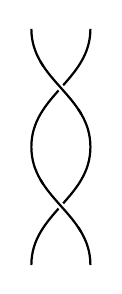
\begin{tikzpicture}
    \begin{knot}
      \strand[thick] (0,0)
        to [out=down,in=up] (0.75,-1.5)
        to [out=down,in=up] (0,-3);
      \strand[thick] (0.75,0)
        to [out=down,in=up] (0,-1.5)
        to [out=down,in=up] (0.75,-3);
      \flipcrossings{2}
    \end{knot}
  \end{tikzpicture}
\] and make it look like \[
  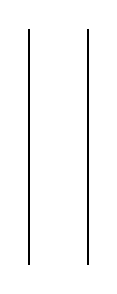
\begin{tikzpicture}
    \begin{knot}
      \strand[thick] (0,0)
        to (0,-3);
      \strand[thick] (0.75,0)
        to (0.75,-3);
    \end{knot}
  \end{tikzpicture}
\] so the linking number in 4 dimensions is only defined \(\mod 2\).
Thus the ``Hopf invariant'' is only defined \(\mod 2\).

The exact same thing happens in higher dimensions, too, so in fact we
have:
\[\pi_{k+1}(S^k) = \mathbb{Z}/2 \quad\text{for any}\quad k \geqslant 3.\]
This illustrates an important general fact: when the dimensions get high
enough, there's more room to wiggle things around, and as we keep
jacking up the dimension, homotopy groups simplify a bit and settle down
after a while. This is the idea behind ``stable homotopy theory''.

Let's look at some more examples. We have

\begin{itemize}
\tightlist
\item
  \(\pi_3(S^1) = \{0\}\)
\item
  \(\pi_4(S^2) = \mathbb{Z}/2\)
\item
  \(\pi_5(S^3) = \mathbb{Z}/2\)
\item
  \(\pi_6(S^4) = \mathbb{Z}/2\)
\end{itemize}

and so on:

\[\pi_{k+2}(S^k) = \mathbb{Z}/2 \quad\text{for any}\quad k\geqslant 2\]

Sadly, I do \emph{not} understand why this is true. How do you wrap a
4-sphere around a 2-sphere in an interesting way? Dunno.

(Thanks to Dan Christensen, an answer appears at the end of this post.)

Plunging on undeterred, we have:

\begin{itemize}
\tightlist
\item
  \(\pi_4(S^1) = \{0\}\)
\item
  \(\pi_5(S^2) = \mathbb{Z}/2\)
\item
  \(\pi_6(S^3) = \mathbb{Z}/12\)
\item
  \(\pi_7(S^4) = \mathbb{Z}\oplus\mathbb{Z}/12\)
\item
  \(\pi_8(S^5) = \mathbb{Z}/24\)
\item
  \(\pi_9(S^6) = \mathbb{Z}/24\)
\end{itemize}

and so on:

\[\pi_{k+3}(S^k) = \mathbb{Z}/24 \quad\text{for any}\quad k\geqslant 5.\]

Here is where the magic number 24 comes in! What the above says is that
if \(k\) is large enough, there are exactly 24 different homotopy class
of maps from an \((k+3)\)-sphere to an \(k\)-sphere!

Now I should explain what this has to do with string theory. But first I
should say more about the homotopy groups of spheres. There are some
simple patterns worth knowing about. First,
\[\pi_m(S^1) = \{0\} \quad\text{for any}\quad m\geqslant 2.\] Second,
there is a nice formula for when the homotopy groups settle down as we
jack up the dimension:
\[\mbox{$\pi_{k+n}(S^k)$ is independent of $k$ as long as $k\geqslant n+2$.}\]
The homotopy groups can stabilize sooner, as we saw for \(n = 2\), but
never later, and often they stabilize right at \(k = n+2\). There is a
simple reason for this. We saw that \(\pi_{k+1}(S^k)\) stabilized at
\(k = 3\) because it's easy to unlink links in 4 or more dimensions.
Similarly, \(\pi_{k+n}(S^k)\) must stabilize by the time \(k = n+2\),
because it's easy to untie knotted \(n\)-dimensional surfaces in
\(2n+2\) or more dimensions!

For more on stable homotopy groups of spheres, try:

\begin{enumerate}
\def\labelenumi{\arabic{enumi})}
\setcounter{enumi}{1}
\item
  Douglas C. Ravenel, \emph{Complex cobordism and stable homotopy groups
  of spheres}, Academic Press, Orlando, 1986.

  Douglas C. Ravenel, \emph{Nilpotence and periodicity in stable
  homotopy theory}, Princeton University Press, Princeton, 1992.
\end{enumerate}

Ravenel also spoke at this conference and is a real expert on stable
homotopy groups of spheres. Unfortunately his talk was too high-powered
for me. The 2nd book above is a bit more forgiving to the amateur, but
the first one has lots of nice tables of stable homotopy groups of
spheres.

The relationship between homotopy groups of spheres and higher-
dimensional knot theory is a wonderful thing. James Dolan and I are
learning a lot about \(n\)-categories by pondering it. When I spoke to
him at the conference at Northwestern, it became clear that Andre Joyal
had also thought about it very deeply. Joyal is famous for his work
relating category theory, combinatorics and topology, and his way of
thinking about the homotopy groups of spheres reflects these interests.
He said a very fascinating thing; he said ``really we should call the
sphere spectrum the `true integers'\,''. I would like to explain
this\ldots{} but here things get a bit technical, and I am afraid they
will get a lot more technical when I get around to the string theory
stuff.

What's the ``sphere spectrum''? Well, roughly it's just the list of
spheres \(S^0\), \(S^1\), \(S^2\), \ldots, but the word ``spectrum''
refers to the way all these spaces are all related, all aspects of one
big thing.

Here's a nice way to think of it. Start with the integers. Normally we
think of these as just a set, or actually a group, since we can add
them. But if we avoid the sin of mistaking isomorphism for equality we
can think of them as a category.

I already began to explain this in my parable about the shepherd in
\protect\hyperlink{week99}{``Week 99''}. The shepherd started with the
category of finite sets and ``decategorified'' it to obtain the set of
natural numbers, associating to each finite set a natural number, its
number of elements. Taking disjoint unions of sets corresponds to
addition, the empty set corresponds to zero, and so on.

Okay. What are the \emph{integers} the decategorification of?

Well, we can imagine finite sets that have both ``positive'' and
``negative'' elements. The ``number of elements'' of such a set will be
the number of positive elements minus the number of negative elements.
This is a bit weird if we're talking about sheep, but perhaps not so
weird if we talk about positrons and electrons, which can annihilate
each other. (In \protect\hyperlink{week92}{``Week 92''} I explain what
I'm hinting at here: the relation between antiparticles and
adjunctions.)

Topologists prefer to speak of ``positively and negatively oriented
points''. We can draw a set of positively and negatively oriented points
like this: \[
  \begin{tikzpicture}
    \node at (0,0) {$-$};
    \node at (1,0) {$+$};
    \node at (2,0) {$+$};
    \node at (3,0) {$+$};
    \node at (4,0) {$+$};
    \node at (5,0) {$-$};
    \node at (6,0) {$-$};
  \end{tikzpicture}
\] We can add them by setting them side by side. But how do the
positively and negatively oriented points cancel? Well, remember, we're
trying to get a category! If finite lists of positively and negatively
oriented points are our objects, what are our morphisms? How about
tangles, like this: \[
  \begin{tikzpicture}
    \node[label=above:{$-$}] at (0,0) {};
    \node[label=above:{$+$}] at (1,0) {};
    \node[label=above:{$+$}] at (2,0) {};
    \node[label=above:{$+$}] at (3,0) {};
    \node[label=above:{$+$}] at (4,0) {};
    \node[label=above:{$-$}] at (5,0) {};
    \node[label=above:{$-$}] at (6,0) {};
    \begin{knot}
      \strand[thick] (0,0)
        to [out=down,in=down,looseness=2] (1,0);
      \strand[thick] (0,-3)
        to [out=up,in=up,looseness=2] (1,-3);
      \strand[thick] (2,0) to (2,-3);
      \strand[thick] (3,0)
        to [out=down,in=down,looseness=2] (6,0);
      \strand[thick] (4,0)
        to [out=down,in=down,looseness=2] (5,0);
    \end{knot}
    \node[label=below:{$+$}] at (0,-3) {};
    \node[label=below:{$-$}] at (1,-3) {};
    \node[label=below:{$+$}] at (2,-3) {};
  \end{tikzpicture}
\] These let us cancel or create positive and negative points in pairs.
Voila! The categorified integers! Just as the integers form a monoid
under addition, these form a monoidal category (see
\protect\hyperlink{week89}{``Week 89''} for these concepts). The
monoidal structure here is disjoint union, which we can denote with a
plus sign if we like. Similarly, we can write the empty set as 0.

Above it looks like I'm drawing a 1-dimensional tangle in 2-dimensional
space. To understand the ``commutativity'' of the categorified integers
we should work with 1-dimensional tangles in higher-dimensional space.
If we consider them in 3-dimensional space, we have room to switch
things around: \[
  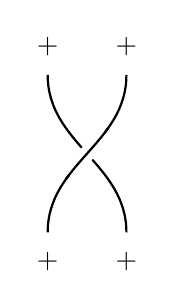
\begin{tikzpicture}
    \begin{knot}[clip width=7]
      \node[label=above:{$+$}] at (0,0) {};
      \node[label=above:{$+$}] at (1,0) {};
      \begin{knot}
        \strand[thick] (1,0)
          to [out=down,in=up] (0,-2);
        \strand[thick] (0,0)
          to [out=down,in=up] (1,-2);
      \end{knot}
      \node[label=below:{$+$}] at (0,-2) {};
      \node[label=below:{$+$}] at (1,-2) {};
    \end{knot}
  \end{tikzpicture}
\] This gets us commutativity, as I explained in
\protect\hyperlink{week100}{``Week 100''}. Technically speaking, we get
a ``braided'' monoidal category. However, there are two different ways
to switch things around; for example, in addition to the above way there
is \[
  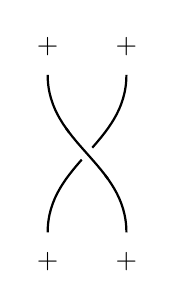
\begin{tikzpicture}
    \begin{knot}[clip width=7]
      \node[label=above:{$+$}] at (0,0) {};
      \node[label=above:{$+$}] at (1,0) {};
      \begin{knot}
        \strand[thick] (0,0)
          to [out=down,in=up] (1,-2);
        \strand[thick] (1,0)
          to [out=down,in=up] (0,-2);
      \end{knot}
      \node[label=below:{$+$}] at (0,-2) {};
      \node[label=below:{$+$}] at (1,-2) {};
    \end{knot}
  \end{tikzpicture}
\] To get rid of this problem (if you consider it a problem) we can work
with 1-dimensional tangles in 4-dimensional space, where we can deform
the first way of switching things to the second. We get a ``symmetric''
monoidal category. Working in higher dimensions doesn't change anything:
things have stabilized.

If we impose the extra condition that the morphisms \[
  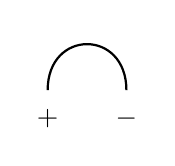
\begin{tikzpicture}
    \begin{knot}
      \strand[thick] (0,0)
        to [out=up,in=up,looseness=2] (1,0);
    \end{knot}
    \node[label=below:{$+$}] at (0,0) {};
    \node[label=below:{$-$}] at (1,0) {};
  \end{tikzpicture}
\] and \[
  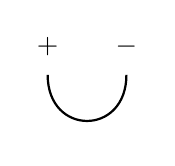
\begin{tikzpicture}
    \begin{knot}
      \strand[thick] (0,0)
        to [out=down,in=down,looseness=2] (1,0);
    \end{knot}
    \node[label=above:{$+$}] at (0,0) {};
    \node[label=above:{$-$}] at (1,0) {};
  \end{tikzpicture}
\] are inverses, as are \[
  \begin{tikzpicture}
    \begin{knot}
      \strand[thick] (0,0)
        to [out=up,in=up,looseness=2] (1,0);
    \end{knot}
    \node[label=below:{$-$}] at (0,0) {};
    \node[label=below:{$+$}] at (1,0) {};
  \end{tikzpicture}
\] and \[
  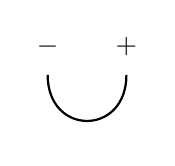
\begin{tikzpicture}
    \begin{knot}
      \strand[thick] (0,0)
        to [out=down,in=down,looseness=2] (1,0);
    \end{knot}
    \node[label=above:{$-$}] at (0,0) {};
    \node[label=above:{$+$}] at (1,0) {};
  \end{tikzpicture}
\] then all morphisms become invertible, so we have not just a monoidal
category but a monoidal groupoid --- a groupoid being a category with
all morphisms invertible (see \protect\hyperlink{week74}{``Week 74''}).
In fact, not only are morphisms invertible, so are all objects! By this
I mean that every object \(x\) has an object \(-x\) such that \(x + -x\)
and \(-x + x\) are isomorphic to \(0\). For example, if \(x\) is the
positively oriented point, \(-x\) is the negatively oriented point, and
vice versa. So we have not just a monoidal groupoid but a ``groupal
groupoid''. (I have adopted this charming terminology from James Dolan.)

Very nice. We seem to have avoided the sin of decategorification, and
are no longer treating the integers as a mere \emph{set} (or group, or
commutative group). We are treating them as a \emph{category} (or
groupal groupoid, or braided groupal groupoid, or symmetric groupal
groupoid).

On the other hand, it's a bit odd to say that \[
  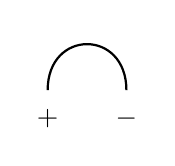
\begin{tikzpicture}
    \begin{knot}
      \strand[thick] (0,0)
        to [out=up,in=up,looseness=2] (1,0);
    \end{knot}
    \node[label=below:{$+$}] at (0,0) {};
    \node[label=below:{$-$}] at (1,0) {};
  \end{tikzpicture}
\] and \[
  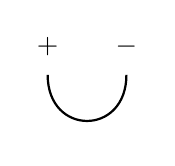
\begin{tikzpicture}
    \begin{knot}
      \strand[thick] (0,0)
        to [out=down,in=down,looseness=2] (1,0);
    \end{knot}
    \node[label=above:{$+$}] at (0,0) {};
    \node[label=above:{$-$}] at (1,0) {};
  \end{tikzpicture}
\] are inverses. This amounts to saying that the morphism: \[
  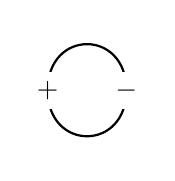
\begin{tikzpicture}
    \begin{knot}
      \strand[thick] (0,0)
        to [out=up,in=up,looseness=2] (1,0);
      \strand[thick] (0,0)
        to [out=down,in=down,looseness=2] (1,0);
    \end{knot}
    \node[fill=white] at (0,0) {$+$};
    \node[fill=white] at (1,0) {$-$};
  \end{tikzpicture}
\] is equal to the identity morphism from 0 to 0, which corresponds to
the empty picture: \[\phantom{.}\] Hmm. They sure don't \emph{look}
equal. We must be doing something wrong.

What are we doing wrong? We're committing the sin of decategorification:
treating isomorphisms as equations! We should treat the integers not as
a mere category, but as a 2-category! See
\protect\hyperlink{week80}{``Week 80''} for the precise definition of
this concept; for now, it's enough to say that a 2-category has things
called 2-morphisms going between morphisms. If we treat the integers as
a 2-category, we can say there is a 2-morphism going from \[
  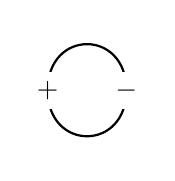
\begin{tikzpicture}
    \begin{knot}
      \strand[thick] (0,0)
        to [out=up,in=up,looseness=2] (1,0);
      \strand[thick] (0,0)
        to [out=down,in=down,looseness=2] (1,0);
    \end{knot}
    \node[fill=white] at (0,0) {$+$};
    \node[fill=white] at (1,0) {$-$};
  \end{tikzpicture}
\] to the identity morphism. This 2-morphism has a nice geometrical
description in terms of a 2-dimensional surface: the surface in 3d space
that's traced out as the above picture shrinks down to the empty
picture. It's hard to draw, but let me try: \[
  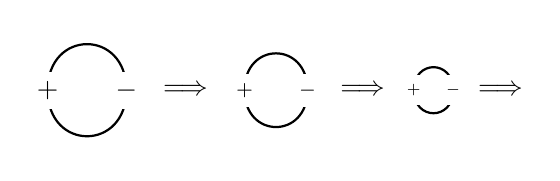
\begin{tikzpicture}
    \begin{scope}
      \begin{knot}
        \strand[thick] (0,0)
          to [out=up,in=up,looseness=2] (1,0);
        \strand[thick] (0,0)
          to [out=down,in=down,looseness=2] (1,0);
      \end{knot}
      \node[fill=white] at (0,0) {$+$};
      \node[fill=white] at (1,0) {$-$};
    \end{scope}
    \node at (1.75,0) {$\Longrightarrow$};
    \begin{scope}[shift={(2.5,0)},scale=0.8]
      \begin{knot}
        \strand[thick] (0,0)
          to [out=up,in=up,looseness=2] (1,0);
        \strand[thick] (0,0)
          to [out=down,in=down,looseness=2] (1,0);
      \end{knot}
      \node[fill=white] at (0,0) {\mbox{\scriptsize$+$}};
      \node[fill=white] at (1,0) {\mbox{\scriptsize$-$}};
    \end{scope}
    \node at (4,0) {$\Longrightarrow$};
    \begin{scope}[shift={(4.65,0)},scale=0.5]
      \begin{knot}
        \strand[thick] (0,0)
          to [out=up,in=up,looseness=2] (1,0);
        \strand[thick] (0,0)
          to [out=down,in=down,looseness=2] (1,0);
      \end{knot}
      \node[fill=white] at (0,0) {\mbox{\tiny$+$}};
      \node[fill=white] at (1,0) {\mbox{\tiny$-$}};
    \end{scope}
    \node at (5.75,0) {$\Longrightarrow$};
  \end{tikzpicture}
\] Okay, say we do this: treat the integers as a 2-category. We again
are faced with a question: do we make all the 2-morphisms invertible? If
we do, we get a ``2-groupoid'', or actually a ``groupal 2-groupoid''.
But again, to do so amounts to committing the sin of decategorification.
To avoid this sin, we should tread the integers as a 3-category. Etc,
etc!

You may have noted how worlds of ever higher-dimensional topology are
automatically unfolding from our attempt to avoid the sin of
decategorification. This is what's so neat about \(n\)-categories. I
haven't told you how it all works, but let me summarize what's actually
happening here. Normally we treat the integers as the free group on one
generator, or else the free commutative group on one generator. But
groups and commutative groups are just the tip of the iceberg! The
following picture is similar to that in
\protect\hyperlink{week74}{``Week 74''}:

\begin{longtable}[]{@{}llll@{}}
\caption{\(k\)-tuply groupal \(n\)-groupoids}\tabularnewline
\toprule
\begin{minipage}[b]{0.26\columnwidth}\raggedright
\strut
\end{minipage} & \begin{minipage}[b]{0.21\columnwidth}\raggedright
\(n=0\)\strut
\end{minipage} & \begin{minipage}[b]{0.21\columnwidth}\raggedright
\(n=1\)\strut
\end{minipage} & \begin{minipage}[b]{0.21\columnwidth}\raggedright
\(n=2\)\strut
\end{minipage}\tabularnewline
\midrule
\endfirsthead
\toprule
\begin{minipage}[b]{0.26\columnwidth}\raggedright
\strut
\end{minipage} & \begin{minipage}[b]{0.21\columnwidth}\raggedright
\(n=0\)\strut
\end{minipage} & \begin{minipage}[b]{0.21\columnwidth}\raggedright
\(n=1\)\strut
\end{minipage} & \begin{minipage}[b]{0.21\columnwidth}\raggedright
\(n=2\)\strut
\end{minipage}\tabularnewline
\midrule
\endhead
\begin{minipage}[t]{0.26\columnwidth}\raggedright
\(k=0\)\strut
\end{minipage} & \begin{minipage}[t]{0.21\columnwidth}\raggedright
sets\strut
\end{minipage} & \begin{minipage}[t]{0.21\columnwidth}\raggedright
groupoids\strut
\end{minipage} & \begin{minipage}[t]{0.21\columnwidth}\raggedright
2-groupoids\strut
\end{minipage}\tabularnewline
\begin{minipage}[t]{0.26\columnwidth}\raggedright
\strut
\end{minipage} & \begin{minipage}[t]{0.21\columnwidth}\raggedright
\strut
\end{minipage} & \begin{minipage}[t]{0.21\columnwidth}\raggedright
\strut
\end{minipage} & \begin{minipage}[t]{0.21\columnwidth}\raggedright
\strut
\end{minipage}\tabularnewline
\begin{minipage}[t]{0.26\columnwidth}\raggedright
\(k=1\)\strut
\end{minipage} & \begin{minipage}[t]{0.21\columnwidth}\raggedright
groups\strut
\end{minipage} & \begin{minipage}[t]{0.21\columnwidth}\raggedright
groupal groupoids\strut
\end{minipage} & \begin{minipage}[t]{0.21\columnwidth}\raggedright
groupal 2-groupoids\strut
\end{minipage}\tabularnewline
\begin{minipage}[t]{0.26\columnwidth}\raggedright
\strut
\end{minipage} & \begin{minipage}[t]{0.21\columnwidth}\raggedright
\strut
\end{minipage} & \begin{minipage}[t]{0.21\columnwidth}\raggedright
\strut
\end{minipage} & \begin{minipage}[t]{0.21\columnwidth}\raggedright
\strut
\end{minipage}\tabularnewline
\begin{minipage}[t]{0.26\columnwidth}\raggedright
\(k=2\)\strut
\end{minipage} & \begin{minipage}[t]{0.21\columnwidth}\raggedright
commutative groups\strut
\end{minipage} & \begin{minipage}[t]{0.21\columnwidth}\raggedright
braided groupal groupoids\strut
\end{minipage} & \begin{minipage}[t]{0.21\columnwidth}\raggedright
braided groupal 2-groupoids\strut
\end{minipage}\tabularnewline
\begin{minipage}[t]{0.26\columnwidth}\raggedright
\strut
\end{minipage} & \begin{minipage}[t]{0.21\columnwidth}\raggedright
\strut
\end{minipage} & \begin{minipage}[t]{0.21\columnwidth}\raggedright
\strut
\end{minipage} & \begin{minipage}[t]{0.21\columnwidth}\raggedright
\strut
\end{minipage}\tabularnewline
\begin{minipage}[t]{0.26\columnwidth}\raggedright
\(k=3\)\strut
\end{minipage} & \begin{minipage}[t]{0.21\columnwidth}\raggedright
" "\strut
\end{minipage} & \begin{minipage}[t]{0.21\columnwidth}\raggedright
symmetric groupal groupoids\strut
\end{minipage} & \begin{minipage}[t]{0.21\columnwidth}\raggedright
weakly involutory groupal 2-groupoids\strut
\end{minipage}\tabularnewline
\begin{minipage}[t]{0.26\columnwidth}\raggedright
\strut
\end{minipage} & \begin{minipage}[t]{0.21\columnwidth}\raggedright
\strut
\end{minipage} & \begin{minipage}[t]{0.21\columnwidth}\raggedright
\strut
\end{minipage} & \begin{minipage}[t]{0.21\columnwidth}\raggedright
\strut
\end{minipage}\tabularnewline
\begin{minipage}[t]{0.26\columnwidth}\raggedright
\(k=4\)\strut
\end{minipage} & \begin{minipage}[t]{0.21\columnwidth}\raggedright
" "\strut
\end{minipage} & \begin{minipage}[t]{0.21\columnwidth}\raggedright
" "\strut
\end{minipage} & \begin{minipage}[t]{0.21\columnwidth}\raggedright
strongly involutory groupal 2-groupoids\strut
\end{minipage}\tabularnewline
\begin{minipage}[t]{0.26\columnwidth}\raggedright
\strut
\end{minipage} & \begin{minipage}[t]{0.21\columnwidth}\raggedright
\strut
\end{minipage} & \begin{minipage}[t]{0.21\columnwidth}\raggedright
\strut
\end{minipage} & \begin{minipage}[t]{0.21\columnwidth}\raggedright
\strut
\end{minipage}\tabularnewline
\begin{minipage}[t]{0.26\columnwidth}\raggedright
\(k=5\)\strut
\end{minipage} & \begin{minipage}[t]{0.21\columnwidth}\raggedright
" "\strut
\end{minipage} & \begin{minipage}[t]{0.21\columnwidth}\raggedright
" "\strut
\end{minipage} & \begin{minipage}[t]{0.21\columnwidth}\raggedright
" "\strut
\end{minipage}\tabularnewline
\bottomrule
\end{longtable}

What are all these things? Well, an \(n\)-groupoid is an \(n\)-category
with all morphisms invertible, at least up to equivalence. An
\((k+n)\)-groupoid with only trivial \(j\)-morphisms for \(j < k\) can
be seen as a special sort of \(n\)-groupoid, which we call a
``\(k\)-tuply groupal \(n\)-groupoid''.

Part of Joyal's point was that we should really think of the integers as
the ``free \(k\)-tuply monoidal \(n\)-groupoid on one object''. Here the
idea is not to fix \(n\) and \(k\) once and for all --- this would only
prevent us from understanding the subtleties that show up when we
increase \(n\) and \(k\)! Instead, we should think of them as variable,
or perhaps consider the limit as they become large.

The other part of his point was that there's a correspondence between
\(n\)-groupoids and the information left in topological spaces when we
ignore all homotopy groups above dimension \(n\) --- so-called
``homotopy \(n\)-types''. Using this correspondence, the ``free
\(k\)-tuply monoidal \(n\)-groupoid on one object'' corresponds to the
homotopy \((k+n)\)-type of the \(k\)-sphere. Moreover, if we keep
jacking up \(k\), this stabilizes when \(k\geqslant n+2\). Actually, as
the dittos in the above chart suggest, it's a quite general fact that
the notion of \(k\)-tuply monoidal \(n\)-groupoid stabilizes for
\(k\geqslant n+2\).

Yet another point is that the pictures above explain the relation
between higher-dimensional knot theory and the homotopy groups of
spheres in a very vivid, direct way.

Okay. What about string theory and the magic number 24? Well, notice
that the pictures above started looking a bit like strings! Hmm\ldots.

Here's the idea, as far as I understand it. Presumably all but the hardy
have stopped reading this article by now, so I will pull out all the
stops. The string worldsheet is a Riemann surface so we'll need some
stuff about Riemann surfaces from \protect\hyperlink{week28}{``Week
28''}. Let \(M(g,n)\) be the moduli space of Riemann surfaces with genus
\(g\) and \(n\) punctures, and let \(G(g,n)\) be the corresponding
mapping class group. Since \(M(g,n)\) is the quotient of Teichmueller
space by \(G(g,n)\) and Teichmueller space is contractible, we have
\[M(g,n) = \mathcal{B}G(g,n)\] where ``\(\mathcal{B}\)'' means
``classifying space''. There's a natural inclusion
\[G(g,n)\hookrightarrow G(g+1,n)\] defined by sewing an torus with two
punctures onto your genus-\(g\) surface with \(n\) punctures, which
increases the genus by 1. Let's define \(G(\infty,n)\) to be direct
limit as \(g\to\infty\), and let
\[M(\infty,n) = \mathcal{B}G(\infty,n).\] Now it turns out
\(M(\infty,1)\) has a kind of product on it. The reason is that there
are products \[M(g,1)\times M(h,1)\to M(g+h,1)\] given sewing two
surfaces together with a 3-punctured sphere. Using this product we can
define the group completion \[M(\infty,1)^+\] and the result Tillmann
stated which got me so excited was that
\[\pi_3(M(\infty,1)^+) = \mathbb{Z}/24 \oplus H\] for some unknown group
\(H\). Since this is really a result about the mapping class groups of
surfaces, it \emph{must} have something to do with how conformal field
theories always give projective representations of these mapping class
groups, with the ``phase ambiguity'' being of the form
\(\exp(2\pi ci/24)\), where \(c\) is the ``central charge''. No? I just
don't quite see why. Maybe someone will enlighten me.

Anyway, the way she proved this definitely ties right into the stuff
about stable homotopy groups of spheres. She used explicit maps between
the third stable homotopy group of spheres
\[\pi_{k+3}(S^k) = \mathbb{Z}/24 \quad\text{for}\quad k \geqslant 5\]
and \(\pi_3(M(\infty,1)^+)\)! And the way she got the map from the
latter to the former amounts to working with pictures I was drawing
above. To put it more precisely, in

\begin{enumerate}
\def\labelenumi{\arabic{enumi})}
\setcounter{enumi}{2}
\tightlist
\item
  ``Higher-dimensional algebra and topological quantum field theory'',
  by John Baez and James Dolan, \emph{Jour. Math. Phys.} \textbf{36}
  (1995), 6073--6105.
\end{enumerate}

we argue that framed \(n\)-dimensional surfaces embedded in
\((n+k)\)-dimensions should be described by the free \(k\)-tuply
monoidal \(n\)-category with duals on one object. This should map down
to the free \(k\)-tuply groupal \(n\)-groupoid on one object, by the
usual yoga of ``freeness''. Taking \(n = 3\) and \(k\) sufficiently
large, we should obtain a homomorphism from the mapping class group of
any Riemann surface to the third stable homotopy group of spheres!
Presumably the idea is that in the limit of large genus this
homomorphism is onto!

Of course, Tillmann doesn't prove her result using the still-nascent
formalism of \(n\)-categories, but I think it will eventually be
possible. (Also, my rough argument applies to Riemann surfaces with no
punctures, while she considers those with one puncture, but various
things she said make me think this might not be such a big deal.) The
real puzzle is this: what does \[\pi_3(M(\infty,n)^+)\] have to do with
central extensions of \(G(g,n)\) for finite \(g\)? If I could figure
this out I'd be very happy.

\begin{center}\rule{0.5\linewidth}{0.5pt}\end{center}

\textbf{Addendum:} Dan Christensen answered a puzzle above. Here's how
to get a nontrivial element of \[\pi_4(S^2).\] Take the map
\(f\colon S^3\to S^2\) generating \[\pi_3(S^2)\] and compose it with the
map \(g\colon S^4\to S^3\) generating \[\pi_4(S^3)\] (which, by the way,
is obtained from \(f\) by ``suspension'') to obtain the desired map from
\(S^4\) to \(S^2\). This is an instance of a very general trick:
composing elements of homotopy groups of spheres to get new ones!

\begin{center}\rule{0.5\linewidth}{0.5pt}\end{center}

\emph{Think of one and minus one. Together they add up to zero, nothing,
nada, niente, right? Picture them together, then picture them
separating, peeling part\ldots. Now you have something, you have two
somethings, where you once had nothing.} - John Updike, Roger's Version

\[
  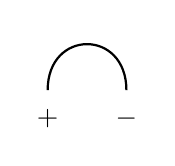
\begin{tikzpicture}
    \begin{knot}
      \strand[thick] (0,0)
        to [out=up,in=up,looseness=2] (1,0);
    \end{knot}
    \node[label=below:{$+$}] at (0,0) {};
    \node[label=below:{$-$}] at (1,0) {};
  \end{tikzpicture}
\]
\hypertarget{week103}{%
\section{April 26, 1997}\label{week103}}

As I segue over from the homotopy theory conference at Northwestern
University to the conference on higher-dimensional algebra and physics
that took place right after that, it's a good time to mention Ronnie
Brown's web page:

\begin{enumerate}
\def\labelenumi{\arabic{enumi})}
\tightlist
\item
  Ronald Brown, Higher-dimensional group theory,
  \texttt{http://www.bangor.ac.uk/\textasciitilde{}mas010/home.html}
\end{enumerate}

Brown is the one who coined the phrase ``higher-dimensional algebra'',
and for many years he has been developing this subject, primarily as a
tool for doing homotopy theory. I wrote a bit about his ideas two years
ago, in \protect\hyperlink{week53}{``Week 53''}. A lot has happened in
higher-dimensional algebra since then, and the web page above is a good
place to get an overview of it. It includes a nice bibliography on the
subject. Also, if you find the math a bit strenuous, you can rest your
brain and delight your eyes at the related site:

\begin{enumerate}
\def\labelenumi{\arabic{enumi})}
\setcounter{enumi}{1}
\tightlist
\item
  Symbolic sculptures and mathematics,
  \texttt{http://www.bangor.ac.uk/SculMath/}
\end{enumerate}

which opens with a striking image of rotating linked tori, and includes
pictures of the mathematical sculpture of John Robinson.

The Workshop on Higher Category Theory and Physics was exciting because
it pulled together a lot of people working on the interface between
these two subjects, many of whom had never before met. It was organized
by Ezra Getzler and Mikhail Kapranov. Getzler is probably most
well-known for his proof of the Atiyah-Singer index theorem. This
wonderful theorem captured the imagination of mathematical physicists
for many years starting in the 1960s. The reason is that it relates the
topology of manifolds to the the solutions of partial differential
equations on these manifolds, and thus ushered in a new age of
applications of topology to physics. In the 1980s, working with ideas
that Witten came up with, Getzler found a nice ``supersymmetric proof''
of the Atiyah-Singer theorem. Later Getzler turned to other things, such
as the use of ``operads'' (see \protect\hyperlink{week42}{``Week 42''})
to study conformal field theory (which shows up naturally in string
theory). Kapranov has also done a lot of work with operads and conformal
field theory, and many other things, but I first learned about him
through his paper with Voevodsky on ``braided monoidal 2-categories''
(see \protect\hyperlink{week4}{``Week 4''}). This got me very excited
since it turned me on to many of the main themes of \(n\)-category
theory.

Alas, my description of this fascinating conference will be terse and
dry in the extreme, since I am flying to Warsaw in 3 hours for a quantum
gravity workshop. I'll just mention a few papers that cover some of the
themes of this conference. Ross Street gave two talks on Batanin's
definition of weak \(n\)-categories (and even weak
\(\omega\)-categories), which one can get as follows:

\begin{enumerate}
\def\labelenumi{\arabic{enumi})}
\setcounter{enumi}{2}
\tightlist
\item
  Ross Street, \emph{The role of Michael Batanin's monoidal globular
  categories.} ``Lecture I: Globular categories and trees''. ``Lecture
  II: Higher operads and weak \(\omega\)-categories''. Available in
  gzipped Postscript form at
  \texttt{http://www.math.mq.edu.au/\textasciitilde{}street/Publications.html}
\end{enumerate}

Subsequently Batanin has written a more thorough paper on his
definition:

\begin{enumerate}
\def\labelenumi{\arabic{enumi})}
\setcounter{enumi}{3}
\tightlist
\item
  Michael Batanin, ``Monoidal globular categories as a natural
  environment for the theory of weak \(n\)-categories'', \emph{Adv.
  Math} \textbf{136} (1998), 39--103, preprint available at
  \texttt{http://www-math.mpce.mq.edu.au/\textasciitilde{}mbatanin/papers.html}
\end{enumerate}

I gave a talk on Dolan's and my definition of weak \(n\)-categories,
which one can get as follows:

\begin{enumerate}
\def\labelenumi{\arabic{enumi})}
\setcounter{enumi}{4}
\tightlist
\item
  John Baez, ``An introduction to \(n\)-categories'', to appear in the
  proceedings of \emph{Category Theory and Computer Science '97},
  preprint available as
  \href{http://xxx.lanl.gov/abs/q-alg/9705009}{\texttt{q-alg/9705009}}
  or in Postscript form at
  \texttt{http://math.ucr.edu/home/baez/ncat.ps}
\end{enumerate}

Unfortunately Tamsamani was not there to present \emph{his} definition
of weak \(n\)-categories, but at least I have learned how to get his
papers electronically:

\begin{enumerate}
\def\labelenumi{\arabic{enumi})}
\setcounter{enumi}{5}
\item
  Zouhair Tamsamani, ``Sur des notions de \(\infty\)-categorie et
  \(\infty\)-groupoide non-strictes via des ensembles
  multi-simpliciaux'', preprint available as
  \href{http://xxx.lanl.gov/abs/alg-geom/9512006}{\texttt{alg-geom/9512006}}.

  Zouhair Tamsamani, ``Equivalence de la theorie homotopique des
  \(n\)-groupoides et celle des espaces topologiques \(n\)-tronques'',
  preprint available as
  \href{http://xxx.lanl.gov/abs/alg-geom/9607010}{\texttt{alg-geom/9607010}}.
\end{enumerate}

Also, Carlos Simpson has written an interesting paper using Tamsamani's
definition:

\begin{enumerate}
\def\labelenumi{\arabic{enumi})}
\setcounter{enumi}{6}
\tightlist
\item
  Carlos Simpson, ``A closed model structure for \(n\)-categories,
  internal Hom, \(n\)-stacks and generalized Seifert-Van Kampen'',
  preprint available as
  \href{http://xxx.lanl.gov/abs/alg-geom/9704006}{\texttt{alg-geom/9704006}}.
\end{enumerate}

In a different but related direction, Masahico Saito discussed a paper
with Scott Carter and Joachim Rieger in which they come up with a nice
purely combinatorial description of all the ways to embed 2-dimensional
surfaces in 4-dimensional space:

\begin{enumerate}
\def\labelenumi{\arabic{enumi})}
\setcounter{enumi}{7}
\tightlist
\item
  J. Scott Carter, Joachim H. Rieger and Masahico Saito, ``A
  combinatorial description of knotted surfaces and their isotopies'',
  to appear in \emph{Adv. Math.}, preprint available at
  \texttt{http://www.math.usf.edu/\textasciitilde{}saito/home.html}
\end{enumerate}

My student Laurel Langford has translated their work into \(n\)-category
theory and shown that ``unframed unoriented 2-tangles form the free
braided monoidal 2-category on one unframed self-dual object'':

\begin{enumerate}
\def\labelenumi{\arabic{enumi})}
\setcounter{enumi}{8}
\tightlist
\item
  John Baez and Laurel Langford, ``2-Tangles'', preprint available as
  \href{http://xxx.lanl.gov/abs/q-alg/9703033}{\texttt{q-alg/9703033}}
  and in Postscript form at
  \texttt{http://math.ucr.edu/home/baez/2tang.ps}
\end{enumerate}

This paper summarizes the results; the proofs will appear later.

While I was there, Carter also gave me a very nice paper he'd done with
Saito and Louis Kauffman. This paper discusses 4-manifolds and also
2-dimensional surfaces in 3-dimensional space, again getting a purely
combinatorial description which is begging to be translated into
\(n\)-category theory:

\begin{enumerate}
\def\labelenumi{\arabic{enumi})}
\setcounter{enumi}{9}
\tightlist
\item
  J. Scott Carter, Louis H. Kauffman and Masahico Saito,
  ``Diagrammatics, singularities, and their algebraic interpretations'',
  preprint available at
  \texttt{http://www.math.usf.edu/\textasciitilde{}saito/home.html}
\end{enumerate}

I am sorry not to describe these papers in more detail, but I've been
painfully busy lately. (In fact, I am trying to figure out how to reform
my life to give myself more spare time. I think the key is to say ``no''
more often.)

Thanks to Justin Roberts for pointing out an error in
\protect\hyperlink{week102}{``Week 102''}. The phase ambiguity in
conformal field theories is not necessarily a 24th root of unity; it's
\(\exp(2\pi ic/24)\) where \(c\) is the central charge of the associated
Virasoro representation. This is a big hint as far as my puzzle goes.

Also I thank Dan Christensen for helping me understand \(\pi_4(S^2)\) in
a simpler way, and Scott Carter for a fascinating letter on the themes
of \protect\hyperlink{week102}{``Week 102''}. Alas, I have been too busy
to reply adequately to these nice emails!

Gotta run\ldots.

\begin{center}\rule{0.5\linewidth}{0.5pt}\end{center}
\hypertarget{week104}{%
\section{June 8, 1997}\label{week104}}

A couple of months ago I flew up to Corvallis, Oregon to an AMS meeting.
The AMS, in case you're unfamiliar with it, is the American Mathematical
Society. They have lots of regional meetings with special sessions on
various topics. One reason I went to this one is that there was a
special session on octonions, organized by Tevian Dray and Corinne
Manogue.

After the real numbers come the complex numbers, and after the complex
numbers come the quaternions, and after the quaternions come the
octonions, the most mysterious of all. The real numbers, complex
numbers, and quaternions have lots of applications to physics. What
about the octonions? Aren't they good for something too? This question
has been bugging me for a while now.

In fact, it bugs me so much that I decided to go to Corvallis to look
for clues. After all, in addition to Tevian Dray and Corinne Manogue ---
the former a mathematician, the latter a physicist, both deeply
interested in octonions --- a bunch of other octonion experts were going
to be there. One was my friend Geoffrey Dixon. I told you about him in
\protect\hyperlink{week59}{``Week 59''}. He wrote a book on the complex
numbers, quaternions and octonions and their role in physics. He has a
theory of physics in which these are related to electromagnetism, the
weak force, and the strong force, respectively. It's a bit far out, but
far from crazy! In fact, it's fascinating.

After writing about his book I got in touch with him in Cambridge,
Massachusetts. I found out that his other main interest in life, besides
the octonions, is the game Myst. This is probably not a coincidence. In
both the main question is ``What the heck is really going on here?'' He
has Myst all figured out, but he loves watching people play it, so he
got me to play it for a while. Someday I will buy a CD-ROM drive and
waste a few weeks on that game. Anyway, I got to know him back in the
summer of 1995, so it was nice to see him again in Corvallis.

Another octonion expert is Tony Smith. He too has a far-out but
fascinating theory of physics involving octonions! I wrote about his
stuff in \protect\hyperlink{week91}{``Week 91''}. I had never met him
before the Corvallis conference, but I instantly recognized him when I
met him, because there's a picture of him wearing a cowboy hat on his
homepage. It turns out he always wears that hat. He is a wonderful
repository of information concerning octonions and other interesting
things. He is also a very friendly and laid-back sort of guy. He lives
in Atlanta, Georgia.

I also met another octonion expert I hadn't known about, Tony Sudbery,
from York. (The original York, not the ``new'' one.) He gave a talk on
``The Exceptions that Prove the Rule''. The octonions are related to a
host of other mathematical structures in a very spooky way. In all sorts
of contexts, you can classify algebraic structures and get a nice
systematic infinite list together with a finite number of exceptions.
What's spooky is how the exceptions in one context turn out to be
related to the exceptions in some other context. These relationships are
complicated and mysterious in themselves. It's as if there were a hand
underneath the water and all we see is the fingers poking out here and
there. There seems to be some ``unified theory of exceptions'' waiting
to be discovered, and the octonions must have something to do with it. I
figure that to really understand what the octonions are good for, we
need to understand this ``unified theory of exceptions''.

Let's start by recalling what the octonions are!

I presume you know the real numbers. The complex numbers are things like
\[a + bi\] where \(a\) and \(b\) are real. We can multiply them using
the rule \[i^2 = -1\] They may seem mysterious when you first meet them,
but they lose their mystery when you see they are just a nice way of
keeping track of rotations in the plane.

Similarly, the quaternions are guys like \[a + bi + cj + dk\] which we
can multiply using the rules \[i^2 = j^2 = k^2 = -1\] and \[
  \begin{gathered}
    ij = k, jk = i, ki = j,
  \\ji = -k, kj = -i, ik = -j
  \end{gathered}
\] They aren't commutative, but they are still associative. Again they
may seem mysterious at first, but they lose their mystery when you see
that they are just a nice way of keeping track of rotations in 3 and 4
dimensions. Rotations in more than 2 dimensions don't commute in
general, so the quaternions had \emph{better} not commute. In fact,
Hamilton didn't invent the quaternions to study rotations --- his goal
was merely to cook up a ``division algebra'', where you could divide by
any nonzero element (see \protect\hyperlink{week82}{``Week 82''}).
However, after he discovered the quaternions, he used them to study
rotations and angular momentum. Nowadays people tend instead to use the
vector cross product, which was invented later by Gibbs. The reason is
that in the late 1800s there was a big battle between the fans of
quaternions and the fans of vectors, and the quaternion crowd lost. For
more on the history of this stuff, see:

\begin{enumerate}
\def\labelenumi{\arabic{enumi})}
\tightlist
\item
  Michael J. Crowe, \emph{A History of Vector Analysis}, University of
  Notre Dame, Notre Dame, 1967.
\end{enumerate}

Octonions were invented by Cayley later on in the 1800s. For these, we
start with \emph{seven} square roots of \(-1\), say \(e_1\) up to
\(e_7\). To learn how multiply these, draw the following diagram:
\[\includegraphics{../images/fano.jpg}\] Draw a triangle, draw a line
from each vertex to the midpoint of the opposite edge, and inscribe a
circle in the triangle. Label the 7 points shown with \(e_1\) through
\(e_7\) --- it doesn't matter how, I've just drawn my favorite way. Draw
arrows on the edges of the triangle going around clockwise, draw arrows
on the circle also going around clockwise, and draw arrows on the three
lines pointing from each vertex of the triangle to the midpoint of the
opposite edge. Come on, DO it! I'm doing all this work for you\ldots{}
you should do some, too.

Okay. Now you have your very own octonion multiplication table. Notice
that there are six lines and a circle in your picture. Each one of these
gives us a copy of the quaternions inside the octonions. For example,
say you want to multiply \(e_6\) and \(e_7\). You notice that the the
vertical line says ``\(e_6\), \(e_7\), \(e_2\)'' on it as we follow the
arrow down. Thus, just as for \(i\), \(j\), and \(k\) in the
quaternions, we have \[
  \begin{gathered}
    e6 e7 =  e2,   e7 e2 =  e6,   e2 e6 =  e7
  \\e7 e6 = -e2,   e2 e7 = -e6,   e6 e2 = -e7
  \end{gathered}
\] So in particular we have \(e_6 e_7 = e_2\).

In case you lose your octonion table, don't worry: you don't really need
to remember the \emph{names} of those 7 square roots of \$-1 \$and their
positions on the chart. You just need to remember the geometry of the
chart itself. Names are arbitrary and don't really matter, unless you're
talking to someone else, in which case you have to agree on them.

If you want to see spiffy high-tech octonion multiplication tables,
check out the following websites:

\begin{enumerate}
\def\labelenumi{\arabic{enumi})}
\setcounter{enumi}{1}
\item
  Tony Smith, \texttt{http://galaxy.cau.edu/tsmith/TShome.html}
\item
  Geoffrey Dixon, \texttt{http://www.7stones.com} (Warning: to really
  get into this you need to have at least Netscape 3.0 with Java and
  Shockwave stuff.)
\end{enumerate}

What's so great about the octonions? They are not commutative, and
worse, they are not even \emph{associative}. What's great about them is
that they form a division algebra, meaning you can divide by any nonzero
octonion. Better still, they form a ``normed'' division algebra. Just as
with the reals, complexes, and quaternions, we can define the norm of
the octonion
\[x = a_0 + a_1 e_1 + a_2 e_2 + a_3 e_3 + a_4 e_4 + a_5 e_5 + a_6 e_6 + a_7 e_7\]
to be
\[|x| = \sqrt{a_0^2 + a_1^2 + a_2^2 + a_3^2 + a_4^2 + a_5^2 + a_6^2 + a_7^2}.\]

What makes them a ``normed division algebra'' is that \[|xy| = |x||y|.\]
It's a wonderful fact about the world that the reals, complexes,
quaternions and octonions are the \emph{only} normed division algebras.
That's it!

However, the octonions remain mysterious, at least to me. They are
related to rotations in 7 and 8 dimensions, but not as simply as one
might hope. After all, rotations in \emph{any} number of dimensions are
still associative. Where is this nonassociative business coming from? I
don't really know. This question really bugs me.

A while ago, in \protect\hyperlink{week95}{``Week 95''}, I summarized a
paper by John Schwarz on supersymmetric Yang-Mills theory and why it
works best in dimensions 3, 4, 6, and 10. Basically, only in these
dimensions can you cook up spin-\(1/2\) particles that have as many
physical degrees of freedom as massless spin-\(1\) particles. I sort of
explained why. This in turn allows a symmetry between fermions and gauge
bosons. I didn't explain how \emph{this} works\ldots{} it seems pretty
tricky to me\ldots{} but anyway, it works.

So far, so good. But Schwarz wondered: is it a coincidence that the
numbers 3, 4, 6, and 10 are just two more than the numbers 1, 2, 4, and
8 --- the dimensions of the reals, complexes, quaternions, and
octonions?

Apparently not! The following papers explain what's going on:

\begin{enumerate}
\def\labelenumi{\arabic{enumi})}
\setcounter{enumi}{3}
\item
  Corinne A. Manogue and Joerg Schray, ``Finite Lorentz transformations
  automorphisms, and division algebras'', \emph{Jour. Math. Phys.}
  \textbf{34} (1993), 3746--3767.

  Corinne A. Manogue and Joerg Schray, ``Octonionic representations of
  Clifford algebras and triality'', preprint available as
  \href{http://xxx.lanl.gov/abs/hep-th/9407179}{\texttt{hep-th/9407179}}.
\item
  Anthony Sudbery, ``Division algebras, (pseudo)orthogonal groups and
  spinors'', \emph{Jour. Phys. A} \textbf{17} (1984), 939--955.

  Anthony Sudbery, ``Seven types of incongruity'', handwritten notes.
\end{enumerate}

Here's the basic idea. Let

\begin{itemize}
\tightlist
\item
  \(\mathbb{R}\) be the real numbers
\item
  \(\mathbb{C}\) be the complex numbers
\item
  \(\mathbb{H}\) be the quaternions
\item
  \(\mathbb{O}\) be the octonions
\end{itemize}

Let \(\mathrm{SO}(n,1)\) denote the Lorentz group in \(n+1\) dimensions.
Roughly speaking, this is the symmetry group of \((n+1)\)-dimensional
Minkowski spacetime. Let \(\mathfrak{so}(n,1)\) be the corresponding Lie
algebra (see \protect\hyperlink{week63}{``Week 63''} for a lightning
introduction to Lie algebras). Then it turns out that:

\begin{itemize}
\tightlist
\item
  \(\mathfrak{sl}(2,R) = \mathfrak{so}(2,1)\)
\item
  \(\mathfrak{sl}(2,C) = \mathfrak{so}(3,1)\)
\item
  \(\mathfrak{sl}(2,H) = \mathfrak{so}(5,1)\)
\item
  \(\mathfrak{sl}(2,O) = \mathfrak{so}(9,1)\)
\end{itemize}

This relates reals, complexes, quaternions and octonions to the Lorentz
group in dimensions 3, 4, 6, and 10, and explains the ``coincidence''
noted by Schwarz! But it requires some explanation. Roughly speaking, if
\(\mathrm{SL}(2,\mathbb{K})\) is the group of \(2\times2\) matrices with
determinant \(1\) whose entries lie in the division algebra
\(\mathbb{K} = \mathbb{R}, \mathbb{C}, \mathbb{H}, \mathbb{O}\), then
\(\mathfrak{sl}(2,\mathbb{K})\) is defined to be the Lie algebra of this
group. This is simple enough for \(\mathbb{R}\) or \(\mathbb{C}\).
However, one needs to be careful when defining the determinant of a
\(2\times2\) quaternionic matrix, since quaternions don't commute. One
needs to be even more careful in the octonionic case. Since octonions
aren't even associative, it's far from obvious what the group
\(\mathrm{SL}(2,\mathbb{O})\) would be, so defining the Lie algebra
``\(\mathfrak{sl}(2,\mathbb{O})\)'' requires a certain amount of
finesse. For the details, read the papers.

As Corinne Manogue explained to me, this relation between the octonions
and Lorentz transformations in 10 dimensions suggests some interesting
ways to use octonions in 10-dimensional physics. As we all know, the
10th dimension is where string theorists live. There is also a nice
relation to Geoffrey Dixon's theory. This theory relates the
electromagnetic force to the complex numbers, the weak force to the
quaternions, and the strong force to octonions. How? Well, the gauge
group of electromagnetism is \(\mathrm{U}(1)\), the unit complex
numbers. The gauge group of the weak force is \(\mathrm{SU}(2)\), the
unit quaternions. The gauge group of the strong force is
\(\mathrm{SU}(3)\)\ldots.

Alas, the group \(\mathrm{SU}(3)\) is \emph{not} the unit octonions. The
unit octonions do not form a group since they aren't associative.
\(\mathrm{SU}(3)\) is related to the octonions more indirectly. The
group of symmetries (or technically, ``automorphisms'') of the octonions
is the exceptional group \(\mathrm{G}_2\), which contains
\(\mathrm{SU}(3)\). To get \(\mathrm{SU}(3)\), we can take the subgroup
of \(\mathrm{G}_2\) that preserves a given unit imaginary
octonion\ldots{} say \(e_1\). This is how Dixon relates
\(\mathrm{SU}(3)\) to the octonions.

However, why should one unit imaginary octonion be different from the
rest? Some sort of ``symmetry breaking'', presumably? It seems a bit ad
hoc. However, as Manogue explained, there is a nice way to kill two
birds with one stone. If we pick a particular unit imaginary octonion,
we get a copy of the complex numbers sitting inside the octonions, so we
get a copy of \(\mathfrak{sl}(2,\mathbb{C})\) sitting inside
\(\mathfrak{sl}(2,\mathbb{O})\), so we get a copy of
\(\mathfrak{so}(3,1)\) sitting inside \(\mathfrak{so}(9,1)\)! In other
words, we get a particular copy of the good old 4-dimensional Lorentz
group sitting inside the 10-dimensional Lorentz group. So fixing a unit
imaginary octonion not only breaks the octonion symmetry group
\(\mathrm{G}_2\) down to the strong force symmetry group
\(\mathrm{SU}(3)\), it might also get us from 10-dimensional physics
down to 4-dimensional physics.

Cool, no? There are obviously a lot of major issues involved in turning
this into a full-fledged theory, and they might not work out. The whole
idea could be completely misguided! But it takes guts to do physics, so
it's good that Tevian Dray and Corinne Manogue are bravely pursuing this
idea.

Upon learning that there is a deep relation between \(\mathbb{R}\),
\(\mathbb{C}\), \(\mathbb{H}\), \(\mathbb{O}\) and the Lorentz group in
dimensions 3, 4, 6, 10, one is naturally emboldened to take seriously a
few more ``coincidences''. For example, in
\protect\hyperlink{week82}{``Week 82''} I described the Clifford
algebras \(C_n\) --- i.e., the algebras generated by \(n\) anticommuting
square roots of \(-1\). These Clifford algebras are relevant to
\(n\)-dimensional \emph{Euclidean} geometry, as opposed to the Clifford
algebras relevant to \(n\)-dimensional \emph{Lorentzian} geometry, which
appeared in \protect\hyperlink{week93}{``Week 93''}. They go like this:

\begin{itemize}
\tightlist
\item
  \(C_0 = \mathbb{R}\)
\item
  \(C_1 = \mathbb{C}\)
\item
  \(C_2 = \mathbb{H}\)
\item
  \(C_3 = \mathbb{H}\oplus\mathbb{H}\)
\item
  \(C_4 = \mathbb{H}(2)\)
\item
  \(C_5 = \mathbb{C}(4)\)
\item
  \(C_6 = \mathbb{R}(8)\)
\item
  \(C_7 = \mathbb{R}(8)\oplus\mathbb{R}(8)\)
\item
  \(C_8 = \mathbb{R}(16)\)
\end{itemize}

where \(\mathbb{K}(n)\) stands for \(n\times n\) matrices with entries
taken from \(\mathbb{K} = \mathbb{R}, \mathbb{C}, \mathbb{H}\), and
``\(\oplus\)'' stands for ``direct sum''. Note that \(C_8\) is the same
as \(16\times16\) matrices with entries taken from \(C_0\). That's part
of a general pattern called ``Bott periodicity'': in general,
\(C_{n+8}\) is the same as \(16\times16\) matrices with entries taken
from \(C_n\).

Now consider the dimension of the smallest real representation of
\(C_n\). It's easy to work this out if you keep in mind that the
smallest representation of \(\mathbb{K}(n)\) or
\(\mathbb{K}(n)\oplus \mathbb{K}(n)\) is on \(\mathbb{K}^n\) --- the
vector space consisting of \(n\)-tuples of elements of \(\mathbb{K}\).
We get

The dimension of the smallest real representation:

\begin{itemize}
\tightlist
\item
  of \(C_0\) is 1
\item
  of \(C_1\) is 2
\item
  of \(C_2\) is 4
\item
  of \(C_3\) is 4
\item
  of \(C_4\) is 8
\item
  of \(C_5\) is 8
\item
  of \(C_6\) is 8
\item
  of \(C_7\) is 8
\item
  of \(C_8\) is 16
\end{itemize}

Note that it increases at \(n = 1, 2, 4, 8\). These are the dimensions
of \(\mathbb{R}\), \(\mathbb{C}\), \(\mathbb{H}\), and \(\mathbb{O}\).
Coincidence?

No! Indeed, \(C_n\) has a representation on a \(k\)-dimensional real
vector space if and only if the unit sphere in that vector space,
\(S^{k-1}\), admits \(n\) linearly independent smooth vector fields. So
the above table implies that:

\begin{itemize}
\tightlist
\item
  The sphere \(S^0\) admits 0 linearly independent vector fields.
\item
  The sphere \(S^1\) admits 1 linearly independent vector fields.
\item
  The sphere \(S^3\) admits 3 linearly independent vector fields.
\item
  The sphere \(S^7\) admits 7 linearly independent vector fields.
\end{itemize}

These spheres are the unit real numbers, the unit complex numbers, the
unit quaternions, and the unit octonions, respectively! If you know
about normed division algebras, it's obvious that these sphere admit the
maximum possible number of linear independent vector fields: you can
just take a basis of vectors at one point and ``left translate'' it to
get a bunch of linearly independent vector fields.

Now --- Bott periodicity has period 8, and the octonions have dimension
8. And as we've seen, both have a lot to do with Clifford algebras. So
maybe there is a deep relation between the octonions and Bott
periodicity. Could this be true? If so, it would be good news, because
while octonions are often seen as weird exceptional creatures, Bott
periodicity is bigtime, mainstream stuff!

And in fact it \emph{is} true. More on Bott periodicity and the
octonions coming up next Week.

\begin{center}\rule{0.5\linewidth}{0.5pt}\end{center}

\textbf{Addendum:} Robert Helling provided some interesting further
comments on supersymmetric gauge theories and the division algebras,
which I quote below. He recommends the following reference:

\begin{enumerate}
\def\labelenumi{\arabic{enumi})}
\setcounter{enumi}{5}
\tightlist
\item
  J. M. Evans, ``Supersymmetric Yang-Mills theories and division
  algebras'', \emph{Nucl. Phys.} \textbf{B298} (1988), 92--108.
\end{enumerate}

and he writes:

\begin{quote}
Let me add a technical remark that I extract from Green, Schwarz, and
Witten, Vol 1, Appendix 4A.

The appearance of dimensions 3,4,6, and 10 can most easily been seen
when one tries to write down a supersymmetric gauge theory in arbitrary
dimension. This means we're looking for a way to throw in some spinors
to the Lagrangian of a pure gauge theory: \[-1/4 F^2\] in a way that the
new Lagrangian is invariant (up to a total derivative) under some
infinitesimal variations. These describe supersymmetry if their
commutator is a derivative (a generator of spacetime translations). As
usual, we parameterize this variation by a parameter \(\varepsilon\),
but now \(\varepsilon\) is a spinor.

From people that have been doing this for their whole life we learn that
the following Ansatz is common:
\[\delta A_m = i/2 \varepsilon^\dagger \Gamma_m \psi\]
\[\delta \psi = -1/4 F_{mn} \Gamma^{mn} \varepsilon\] Here \(A\) is the
connection, \(F\) its field strength and \(\psi\) a spinor of a type to
be determined. I suppressed group indices on all these fields. They are
all in the adjoint representation. \(\Gamma\) are the generators of the
Clifford algebra described by John Baez before.

{[}Also, \(\varepsilon^\dagger\) is my feeble subsitute for an
\(\varepsilon\) with a bar over it. --- JB{]}

For the Lagrangian we try the usual Yang-Mills term and add a minimally
coupled kinetic term for the fermions:
\[-1/4 F^2 + ig/2 \psi^\dagger \Gamma^m D_m \psi\] Here \(D_m\) is the
gauge covariant derivative and \(g\) is some number that we can tune to
to make this vanish under the above variations. When we vary the first
term we find \(g = 1\). In fact everything cancels without considering a
special dimension except for the term that is trilinear in \(\psi\) that
comes from varying the connection in the covariant derivative in the
fermionic term. This reads something like
\[f_{abc} \varepsilon^\dagger \Gamma_m \psi^a \psi^b \Gamma^m \psi^c\]
where I put in the group indices and the structure constants
\(f_{abc}\). This has to vanish for other reasons since there is no
other trilinear term in the fermions available. And indeed, after you've
written out the antisymmetry of \(f\) explicitly and take out the
spinors since this should vanish for all choices of \(\psi\) and
\(\varepsilon\). We are left with an expression that is only made of
gammas. And in fact, this expression exactly vanishes in dimensions 3,
4, 6, and 10 due to a Fierz identity. (Sorry, I don't have time to work
this out more explicitly.)

This is related to the division algebra as follows (as explained in the
papers pointed out by John Baez): Take for concreteness \(d = 10\). Here
we go to a light-cone frame by using coordinates
\[x^+ = x^0 + x^9 \quad\text{and}\quad x^- = x^0 - x^1.\] Then we write
the \(\Gamma_m\) as block matrices where \(\Gamma_+\) and \(\Gamma_-\)
have the \(+\)/\(-\) unit matrix as blocks and the others have
\(\gamma_i\) as blocks where \(\gamma_i\) are the \(\mathrm{SO}(8)\)
Dirac matrices (\(i=1,...,9\)). But they are intimately related to the
octonions. Remember there is triality in \(\mathrm{SO}(8)\) which means
that we can treat left-handed spinors, right-handed spinors and vectors
on an equal basis (see \href{week61.html}{week61},
\href{week90.html}{week90}, \href{week91.html}{week91}). Now I write out
all three indices of \(\gamma_i\). Because of triality I can use
\(i\),\(j\),\(k\) for spinor, dotted spinor and vector indices. Then it
is known that \[
  \gamma_{ijk} =
  \begin{cases}
    c_{ijk} &\mbox{for $i,j,k<8$;}
  \\\delta_{ij} &\mbox{for $k=8$ (and $ijk$ permuted);}
  \\0 &\mbox{for more than two of $ijk$ equal to $8$.}
  \end{cases}
\] is a representation of \(\mathrm{Cliff}(8)\) if \(c_{ijk}\) are the
structure constants of the octonions (i.e.~\(e_i e_j = c_{ijk} e_k\) for
the 7 roots of \(-1\) in the octonions).

When you plug this representation of the \(\Gamma\)'s in the above
mentioned \(\gamma\) expression you will will find that it vanishes due
to the antisymmetry of the associator \[[a,b,c] = a(bc) - (ab)c\]

in the division algebras. This is my understanding of the relation of
supersymmetry to the divison algebras.

Robert
\end{quote}

\begin{center}\rule{0.5\linewidth}{0.5pt}\end{center}
\hypertarget{week105}{%
\section{June 21, 1997}\label{week105}}

There are some spooky facts in mathematics that you'd never guess in a
million years\ldots{} only when someone carefully works them out do they
become clear. One of them is called ``Bott periodicity''.

A 0-dimensional manifold is pretty dull: just a bunch of points.
1-dimensional manifolds are not much more varied: the only possibilities
are the circle and the line, and things you get by taking a union of a
bunch of circles and lines. 2-dimensional manifolds are more
interesting, but still pretty tame: you've got your n-holed tori, your
projective plane, your Klein bottle, variations on these with extra
handles, and some more related things if you allow your manifold to go
on forever, like the plane, or the plane with a bunch of handles added
(possibly infinitely many!), and so on\ldots. You can classify all these
things. 3-dimensional manifolds are a lot more complicated: nobody knows
how to classify them. 4-dimensional manifolds are a \emph{lot} more
complicated: you can \emph{prove} that it's \emph{impossible} to
classify them --- that's called Markov's Theorem.

Now, you probably wouldn't have guessed that a lot of things start
getting simpler when you get up around dimension 5. Not everything, just
some things. You still can't classify manifolds in these high
dimensions, but if you make a bunch of simplifying assumptions you sort
of can, in ways that don't work in lower dimensions. Weird, huh? But
that's another story. Bott periodicity is different. It says that when
you get up to 8 dimensions, a bunch of things are a whole lot like in 0
dimensions! And when you get up to dimension 9, a bunch of things are a
lot like they were in dimension 1. And so on - a bunch of stuff keeps
repeating with period 8 as you climb the ladder of dimensions.

(Actually, I have this kooky theory that perhaps part of the reason
topology reaches a certain peak of complexity in dimension 4 is that the
number 4 is halfway between 0 and 8, topology being simplest in
dimension 0. Maybe this is even why physics likes to be in 4 dimensions!
But this is a whole other crazy digression and I will restrain myself
here.)

Bott periodicity takes many guises, and I already described one in
\protect\hyperlink{week104}{``Week 104''}. Let's start with the real
numbers, and then throw in \(n\) square roots of \(-1\), say
\(e_1,\ldots,e_n\). Let's make them ``anticommute'', so
\[e_i e_j = - e_j e_i\] when \(i\) is different from \(j\). What we get
is called the ``Clifford algebra'' \(C_n\). For example, when \(n = 1\)
we get the complex numbers, which we call C. When \(n = 2\) we get the
quaternions, which we call H, for Hamilton. When \(n = 3\) we
get\ldots{} the octonions?? No, not the octonions, since we always
demand that multiplication be associative! We get the algebra consisting
of \emph{pairs} of quaternions! We call that
\(\mathbb{H}\oplus\mathbb{H}\). When \(n = 4\) we get the algebra
consisting of \(2\times2\) \emph{matrices} of quaternions! We call that
\(\mathbb{H}(2)\). And it goes on, like this:

\begin{itemize}
\tightlist
\item
  \(C_0 = \mathbb{R}\)
\item
  \(C_1 = \mathbb{C}\)
\item
  \(C_2 = \mathbb{H}\)
\item
  \(C_3 = \mathbb{H}\oplus\mathbb{H}\)
\item
  \(C_4 = \mathbb{H}(2)\)
\item
  \(C_5 = \mathbb{C}(4)\)
\item
  \(C_6 = \mathbb{R}(8)\)
\item
  \(C_7 = \mathbb{R}(8)\oplus\mathbb{R}(8)\)
\item
  \(C_8 = \mathbb{R}(16)\)
\end{itemize}

Note that by the time we get to \(n = 8\) we just have \(16\times16\)
matrices of real numbers. And that's how it keeps going: \(C_{n+8}\) is
just \(16\times16\) matrices of guys in \(C_n\)! That's Bott periodicity
in its simplest form.

Actually right now I'm in Vienna, at the Schroedinger Institute, and one
of the other people visiting is Andrzej Trautman, who gave a talk the
other day on ``Complex Structures in Physics'', where he mentioned a
nice way to remember the above table. Imagine the day is only 8 hours
long, and draw a clock with 8 hours. Then label it like this: \[
  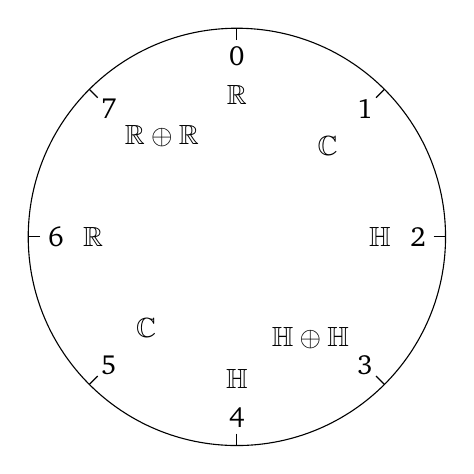
\begin{tikzpicture}
    \draw (0,0) circle[radius=2.65cm];
    \node[label=below:{$\mathbb{R}$}] at (90:2.3) {0};
    \node[label=below left:{$\mathbb{C}$}] at (45:2.3) {1};
    \node[label=left:{$\mathbb{H}$}] at (0:2.3) {2};
    \node[label={[label distance=-2mm]above left:{$\mathbb{H}\oplus\mathbb{H}$}}] at (-45:2.3) {3};
    \node[label=above:{$\mathbb{H}$}] at (-90:2.3) {4};
    \node[label=above right:{$\mathbb{C}$}] at (-135:2.3) {5};
    \node[label=right:{$\mathbb{R}$}] at (180:2.3) {6};
    \node[label={[label distance=-2mm]below right:{$\mathbb{R}\oplus\mathbb{R}$}}] at (135:2.3) {7};
    \foreach \a in {0,45,90,135,180,-135,-90,-45}
      \draw (\a:2.5) to (\a:2.65);
  \end{tikzpicture}
\] The idea here is that as the dimension of space goes up, you go
around the clock. One nice thing about the clock is that it has a
reflection symmetry about the axis from 3 o'clock to 7 o'clock. To use
the clock, you need to know that the dimension of the Clifford algebra
doubles each time you go up a dimension. This lets you figure out, for
example, that the Clifford algebra in 4 dimensions is not really
\(\mathbb{H}\), but \(\mathbb{H}(2)\), since the latter has dimension
\(16 = 2^4\).

Now let's completely change the subject and talk about rotations in
infinite-dimensional space! What's a rotation in infinite-dimensional
space like? Well, let's start from the bottom and work our way up. You
can't really rotate in 0-dimensional space. In 1-dimensional space you
can't really rotate, you can only \emph{reflect} things\ldots{} but we
will count reflections together with rotations, and say that the
operations of multiplying by \(1\) or \(-1\) count as ``rotations'' in
1-dimensional space. In 2-dimensional space we describe rotations by
\(2\times2\) matrices like \[
  \left(
    \begin{array}{cc}
      \cos t & -\sin t
    \\\sin t & \cos t
    \end{array}
  \right)
\] and since we're generously including reflections, also matrices like
\[
  \left(
    \begin{array}{cc}
      \cos t & \sin t
    \\\sin t & -\cos t
    \end{array}
  \right)
\] These are just the matrices whose columns are orthonormal vectors. In
3-dimensional space we describe rotations by \(3\times3\) matrices whose
columns are orthonormal, and so on. In n-dimensional space we call the
set of \(n\times n\) matrices with orthonormal columns the ``orthogonal
group'' \(\mathrm{O}(n)\).

Note that we can think of a rotation in 2 dimensions \[
  \left(
    \begin{array}{cc}
      \cos t & -\sin t
    \\\sin t & \cos t
    \end{array}
  \right)
\] as being a rotation in 3 dimensions if we just stick one more row and
one column like this: \[
  \left(
    \begin{array}{ccc}
      \cos t & -\sin t & 0
    \\\sin t & \cos t & 0
    \\ 0 & 0 & 1
    \end{array}
  \right)
\] This is just a rotation around the z axis. Using the same trick we
can think of any rotation in \(n\) dimensions as a rotation in \(n+1\)
dimensions. So we can think of \(\mathrm{O}(0)\) as sitting inside
\(\mathrm{O}(1)\), which sits inside \(\mathrm{O}(2)\), which sits
inside \(\mathrm{O}(3)\), which sits inside \(\mathrm{O}(4)\), and so
on! Let's do that. Then let's just take the \emph{union} of all these
guys, and we get\ldots{} \(\mathrm{O}(\infty)\)! This is the group of
rotations, together with reflections, in infinite dimensions.

(Now if you know your math, or you read
\protect\hyperlink{week82}{``Week 82''}, you'll realize that I didn't
really change the subject, since the Clifford algebra \(C_n\) is really
just a handy way to study rotations in \(n\) dimensions. But never
mind.)

Now \(\mathrm{O}(\infty)\) is a very big group, but it elegantly
summarizes a lot of information about rotations in all dimensions, so
it's not surprising that topologists have studied it. One of the thing
topologists do when studying a space is to work out its ``homotopy
groups''. If you hand them a space \(X\), and choose a point \(x\) in
this space, they will work out all the topologically distinct ways you
can stick an \(n\)-dimensional sphere in this space, where we require
that the north pole of the sphere be at \(x\). This is what they are
paid to do. We call the set of all such ways the homotopy group
\(\pi_n(X)\). For a more precise description, try
\protect\hyperlink{week102}{``Week 102''} --- but this will do for now.

So, what are the homotopy groups of \(\mathrm{O}(\infty)\)? Well, they
start out looking like this:

\begin{longtable}[]{@{}ll@{}}
\toprule
\(n\) & \(\pi_n(\mathrm{O}(\infty))\)\tabularnewline
\midrule
\endhead
\(0\) & \(\mathbb{Z}/2\)\tabularnewline
\(1\) & \(\mathbb{Z}/2\)\tabularnewline
\(2\) & \(0\)\tabularnewline
\(3\) & \(\mathbb{Z}\)\tabularnewline
\(4\) & \(0\)\tabularnewline
\(5\) & \(0\)\tabularnewline
\(6\) & \(0\)\tabularnewline
\(7\) & \(\mathbb{Z}\)\tabularnewline
\bottomrule
\end{longtable}

And then they repeat, modulo 8. Bott periodicity strikes again!

But what do they mean?

Well, luckily Jim Dolan has thought about this a lot. Discussing it
repeatedly in the little cafe we tend to hang out at, we came up with
the following story. Most of it is known to various people already, but
it came as sort of a revelation to us.

The zeroth entry in the table is easy to understand. \(\pi_0\) keeps
track of how many connected components your space has. The rotation
group \(\mathrm{O}(\infty)\) has two connected components: the guys that
are rotations, and the guys that are rotations followed by a reflection.
So \(\pi_0\) of \(\mathrm{O}(\infty)\) is \(\mathbb{Z}/2\), the group
with two elements. Actually this is also true for \(\mathrm{O}(n)\)
whenever \(n\) is high enough, namely \(1\) or more. So the zeroth entry
is all about ``reflecting''.

The first entry is a bit subtler but very important in physics. It means
that there is a loop in \(\mathrm{O}(\infty)\) that you can't pull
tight, but if you go around that loop \emph{twice}, you trace out a loop
that you \emph{can} pull tight. In fact this is true for
\(\mathrm{O}(n)\) whenever \(n\) is \(3\) or more. This is how there can
be spin-\(1/2\) particles when space is 3-dimensional or higher. There
are lots of nice tricks for seeing that this is true, which I hope the
reader already knows and loves. In short, the first entry is all about
``rotating 360 degrees and not getting back to where you started''.

The second entry is zero.

The third entry is even subtler but also very important in modern
physics. It means that the ways to stick a 3-sphere into
\(\mathrm{O}(\infty)\) are classified by the integers, \(\mathbb{Z}\).
Actually this is true for \(\mathrm{O}(n)\) whenever \(n\) is \(5\) or
more. It's even true for all sorts of other groups, like all ``compact
simple groups''. But can I summarize this entry in a snappy phrase like
the previous nonzero entries? Not really. Actually a lot of applications
of topology to quantum field theory rely on this \(\pi_3\) business. For
example, it's the key to stuff like ``instantons'' in Yang-Mills theory,
which are in turn crucial for understanding how the pion gets its mass.
It's also the basis of stuff like ``Chern-Simons theory'' and ``BF
theory''. Alas, all this takes a while to explain, but let's just say
the third entry is about ``topological field theory in 4 dimensions''.

The fourth entry is zero.

The fifth entry is zero.

The sixth entry is zero.

The seventh entry is probably the most mysterious of all. From one point
of view it is the subtlest, but from another point of view it is
perfectly trivial. If we think of it as being about \(\pi_7\) it's very
subtle: it says that the ways to stick a 7-sphere into
\(\mathrm{O}(\infty)\) are classified by the integers. (Actually this is
true for \(\mathrm{O}(n)\) whenever \(n\) is \(7\) or more.) But if we
keep Bott periodicity in mind, there is another way to think of it: we
can think of it as being about \(\pi_{-1}\), since \(7 = -1 \mod 8\).

But wait a minute! Since when can we talk about \(\pi_n\) when \(n\) is
\emph{negative?!} What's a -1-dimensional sphere, for example?

Well, the idea here is to use a trick. There is a space very related to
\(\mathrm{O}(\infty)\), called \(k\mathrm{O}\). As with
\(\mathrm{O}(\infty)\), the homotopy groups of this space repeat modulo
8. Moreover we have:
\[\pi_n(\mathrm{O}(\infty)) = \pi_{n+1}(k\mathrm{O})\] Combining these
facts, we see that the very subtle \(\pi_7\) of \(\mathrm{O}(\infty)\)
is nothing but the very unsubtle \(\pi_0\) of \(k\mathrm{O}\), which
just keeps track of how many connected components \(k\mathrm{O}\) has.

But what \emph{is} \(k\mathrm{O}\)?

Hmm. The answer is very important and interesting, but it would take a
while to explain, and I want to postpone doing it for a while, so I can
get to the punchline. Let me just say that when we work it all out, we
wind up seeing that the seventh entry in the table is all about
\emph{dimension}.

To summarize:

\begin{itemize}
\tightlist
\item
  \(\pi_0(\mathrm{O}(\infty)) = \mathbb{Z}/2\) is about REFLECTING
\item
  \(\pi_1(\mathrm{O}(\infty)) = \mathbb{Z}/2\) is about ROTATING 360
  DEGREES
\item
  \(\pi_3(\mathrm{O}(\infty)) = \mathbb{Z}\) is about TOPOLOGICAL FIELD
  THEORY IN 4 DIMENSIONS
\item
  \(\pi_7(\mathrm{O}(\infty)) = \mathbb{Z}\) is about DIMENSION
\end{itemize}

But wait! What do those numbers 0, 1, 3, and 7 remind you of?

Well, after I stared at them for a few weeks, they started to remind me
of the numbers 1, 2, 4, and 8. And \emph{that} immediately reminded me
of the reals, the complexes, the quaternions, and the octonions!

And indeed, there is an obvious relationship. Let \(n\) be 1, 2, 4, or
8, and correspondingly let \(\mathbb{A}\) stand for either the reals
\(\mathbb{R}\), the complex numbers \(\mathbb{C}\), the quaternions
\(\mathbb{H}\), or the octonions \(\mathbb{O}\). These guys are
precisely all the ``normed division algebras'', meaning that the obvious
sort of absolute value satisfies \[|xy| = |x||y|.\] Thus if we take any
guy \(x\) in \(\mathbb{A}\) with \(|x| = 1\), the operation of
multiplying by \(x\) is length-preserving, so it's a reflection or
rotation in \(\mathbb{A}\). This gives us a function from the unit
sphere in \(\mathbb{A}\) to \(\mathrm{O}(n)\), or in other words from
the \((n-1)\)-sphere to \(\mathrm{O}(n)\). We thus get nice elements of
\[\pi_0(\mathrm{O}(1)), \quad\pi_1(\mathrm{O}(2)), \quad\pi_3(\mathrm{O}(4)), \quad\pi_7(\mathrm{O}(8))
\] which turn out to be precisely why these particular homotopy groups
of \(\mathrm{O}(\infty)\) are nontrivial.

So now we have the following fancier chart:

\begin{itemize}
\tightlist
\item
  \(\pi_0(\mathrm{O}(\infty))\) is about REFLECTING and the REAL NUMBERS
\item
  \(\pi_1(\mathrm{O}(\infty))\) is about ROTATING 360 DEGREES and the
  COMPLEX NUMBERS
\item
  \(\pi_3(\mathrm{O}(\infty))\) is about TOPOLOGICAL FIELD THEORY IN 4
  DIMENSIONS and the QUATERNIONS
\item
  \(\pi_7(\mathrm{O}(\infty))\) is about DIMENSION and the OCTONIONS
\end{itemize}

Now this is pretty weird. It's not so surprising that reflections and
the real numbers are related: after all, the only ``rotations'' in the
real line are the reflections. That's sort of what \(1\) and \(-1\) are
all about. It's also not so surprising that rotations by 360 degrees are
related to the complex numbers. That's sort of what the unit circle is
all about. While far more subtle, it's also not so surprising that
topological field theory in 4 dimensions is related to the quaternions.
The shocking part is that something so basic-sounding as ``dimension''
should be related to something so erudite-sounding as the ``octonions''!

But this is what Bott periodicity does, somehow: it wraps things around
so the most complicated thing is also the least complicated.

That's more or less the end of what I have to say, except for some
references and some remarks of a more technical nature.

Bott periodicity for \(\mathrm{O}(\infty)\) was first proved by Raoul
Bott in 1959. Bott is a wonderful explainer of mathematics and one of
the main driving forces behind applications of topology to physics, and
a lot of his papers have now been collected in book form:

\begin{enumerate}
\def\labelenumi{\arabic{enumi})}
\tightlist
\item
  \emph{The Collected Papers of Raoul Bott}, ed.~R. D. MacPherson. Vol.
  1: \emph{Topology and Lie Groups (the 1950s)}. Vol. 2:
  \emph{Differential Operators (the 1960s)}. Vol. 3: \emph{Foliations
  (the 1970s)}. Vol. 4: \emph{Mathematics Related to Physics (the
  1980s)}. Birkhauser, Boston, 1994, 2355 pages total.
\end{enumerate}

A good paper on the relation between \(\mathrm{O}(\infty)\) and Clifford
algebras is:

\begin{enumerate}
\def\labelenumi{\arabic{enumi})}
\setcounter{enumi}{1}
\tightlist
\item
  M. F. Atiyah, R. Bott, and A. Shapiro, ``Clifford modules'',
  \emph{Topology} \textbf{3} (1964), 3-38.
\end{enumerate}

For more stuff on division algebras and Bott periodicity try Dave
Rusin's web page, especially his answer to ``Q5. What's the question
with the answer \(n = 1\), \(2\), \(4\), or \(8\)?''

\begin{enumerate}
\def\labelenumi{\arabic{enumi})}
\setcounter{enumi}{2}
\tightlist
\item
  Dave Rusin, ``Binary products, algebras, and division rings'',
  \texttt{http://www.math.niu.edu/\textbackslash{}\textasciitilde{}rusin/known-math/95/division.alg}
\end{enumerate}

Let me briefly explain this \(k\mathrm{O}\) business. The space
\(k\mathrm{O}\) is related to a simpler space called
\(\mathcal{B}\mathrm{O}(\infty)\) by means of the equation
\[k\mathrm{O} = \mathcal{B}\mathrm{O}(\infty)\times\mathbb{Z},\] so let
me first describe \(\mathcal{B}\mathrm{O}(\infty)\). For any topological
group \(G\) you can cook up a space \(\mathcal{B}G\) whose loop space is
homotopy equivalent to \(G\). In other words, the space of
(base-point-preserving) maps from \(S^1\) to \(\mathcal{B}G\) is
homotopy equivalent to \(G\). It follows that
\[\pi_n(G) = \pi_{n+1}(\mathcal{B}G).\] This space \(\mathcal{B}G\) is
called the classifying space of \(G\) because it has a principal
\(G\)-bundle over it, and given \emph{any} decent topological space
\(X\) (say a CW complex) you can get all principal \(G\)-bundles over
\(X\) (up to isomorphism) by taking a map \(f\colon X\to\mathcal{B}G\)
and pulling back this principal \(G\)-bundle over \(\mathcal{B}G\).
Moreover, homotopic maps to \(\mathcal{B}G\) give isomorphic
\(G\)-bundles over \(X\) this way.

Now a principal \(\mathrm{O}(n)\)-bundle is basically the same thing as
an \(n\)-dimensional real vector bundle --- there are obvious ways to go
back and forth between these concepts. A principal
\(\mathrm{O}(\infty)\)-bundle is thus very much like a real vector
bundle of \emph{arbitrary} dimension, but where we don't care about
adding on arbitrarily many 1-dimensional trivial bundles. If we take the
collection of isomorphism classes of real vector bundles over \(X\) and
decree two to be equivalent if they become isomorphic after adding on
trivial bundles, we get something called \(KX\), the ``real K-theory of
X''. It's not hard to see that this is a group. Taking what I've said
and working a bit, it follows that
\[KX = [X, \mathcal{B}\mathrm{O}(\infty)]\] where the right-hand side
means ``homotopy classes of maps from \(X\) to
\(\mathcal{B}\mathrm{O}(\infty)\)''. If we take \(X\) to be \(S^{n+1}\),
we see
\[KS^{n+1} = \pi_{n+1}(\mathcal{B}\mathrm{O}(\infty)) = \pi_n(\mathrm{O}(\infty))\]
It follows that we can get all elements of \(\pi_n\) of
\(\mathrm{O}(\infty)\) from real vector bundles over \(S^{n+1}\).

Of course, the above equations are true only for nonnegative \(n\),
since it doesn't make sense to talk about \(\pi_{-1}\) of a space.
However, to make Bott periodicity work out smoothly, it would be nice if
we could pretend that
\[KS^{-1} = \pi_0(\mathcal{B}\mathrm{O}(\infty)) = \pi_{-1}(\mathrm{O}(\infty)) = \pi_7(\mathrm{O}(\infty)) = \mathbb{Z}\]
Alas, the equations don't make sense, and
\(\mathcal{B}\mathrm{O}(\infty)\) is connected, so we don't have
\(\pi_0(\mathcal{B}\mathrm{O}(\infty)) = \mathbb{Z}\). However, we can
cook up a slightly improved space \(k\mathrm{O}\), which has
\[\pi_n(k\mathrm{O}) = \pi_n(\mathcal{B}\mathrm{O}(\infty))\] when
\(n > 0\), but also has \[\pi_0(k\mathrm{O}) = \mathbb{Z}\] as desired.
It's easy --- we just let
\[k\mathrm{O} = \mathcal{B}\mathrm{O}(\infty)\times\mathbb{Z}.\] So,
let's use this instead of \(\mathcal{B}\mathrm{O}(\infty)\) from now on.

Taking \(n = 0\), we can think of \(S^1\) as \(\mathbb{RP}^1\), the real
projective line, i.e.~the space of 1-dimensional real subspaces of
\(\mathbb{R}^2\). This has a ``canonical line bundle'' over it, that is,
a 1-dimensional real vector bundle which to each point of RP\^{}1
assigns the 1-dimensional subspace of \(\mathbb{R}^2\) that \emph{is}
that point. This vector bundle over \(S^1\) gives the generator of
\(KS^1\), or in other words, \(\pi_0(\mathrm{O}(\infty))\).

Taking \(n = 1\), we can think of \(S^2\) as the ``Riemann sphere'', or
in other words \(\mathbb{CP}^1\), the space of 1-dimensional complex
subspaces of \(\mathbb{C}^2\). This too has a ``canonical line bundle''
over it, which is a 1-dimensional complex vector bundle, or
2-dimensional real vector bundle. This bundle over \(S^2\) gives the
generator of \(KS^2\), or in other words, \(\pi_1(\mathrm{O}(\infty))\).

Taking \(n = 3\), we can think of \(S^4\) as \(\mathbb{HP}^1\), the
space of 1-dimensional quaternionic subspaces of \(\mathbb{H}^2\). The
``canonical line bundle'' over this gives the generator of \(KS^4\), or
in other words, \(\pi_3(\mathrm{O}(\infty))\).

Taking \(n = 7\), we can think of \(S^8\) as \(\mathbb{OP}^1\), the
space of 1-dimensional octonionic subspaces of \(\mathbb{O}^2\). The
``canonical line bundle'' over this gives the generator of \(KS^8\), or
in other words, \(\pi_7(\mathrm{O}(\infty))\).

By Bott periodicity,
\[\pi_7(\mathrm{O}(\infty)) = \pi_8(k\mathrm{O}) = \pi_0(k\mathrm{O})\]
so the canonical line bundle over \(\mathbb{OP}^1\) also defines an
element of \(\pi_0(k\mathrm{O})\). But
\[\pi_0(k\mathrm{O}) = [S^0,k\mathrm{O}] = KS^0\] and \(KS^0\) simply
records the \emph{difference in dimension} between the two fibers of a
vector bundle over \(S^0\), which can be any integer. This is why the
octonions are related to dimension.

If for any pointed space we define \[K^n(X) = K(S^n\wedge X)\] we get a
cohomology theory called K-theory, and it turns out that
\[K^{n+8}(X) = K(X)\] which is another way of stating Bott periodicity.
Now if \(\{*\}\) denotes a single point, \(K(\{*\})\) is a ring (this is
quite common for cohomology theories), and it is generated by elements
of degrees 1, 2, 4, and 8. The generator of degree 8 is just the
canonical line bundle over \(\mathbb{OP}^1\) and multiplication by this
generator gives a map \[K^n(\{*\})\to K^{n+8}(\{*\})\] which is an
isomorphism of groups --- namely, Bott periodicity! In this sense the
octonions are responsible for Bott periodicity.

\begin{center}\rule{0.5\linewidth}{0.5pt}\end{center}

\textbf{Addendum}: The Clifford algebra clock is even better than I
described above, because it lets you work out the fancier Clifford
algebras \(C_{p,q}\), which are generated by \(p\) square roots of
\(-1\) and \(q\) square roots of \(1\), which all anticommute with each
other. These Clifford algebras are good when you have \(p\) dimensions
of ``space'' and \(q\) dimensions of ``time'', and I described the
physically important case where \(q = 1\) in
\protect\hyperlink{week93}{``Week 93''}. To figure them out, you just
work out \(p - q \mod 8\), look at what the clock says for that hour,
and then take \(N\times N\) matrices of what you see, with \(N\) chosen
so that \(C_{p,q}\) gets the right dimension, namely \(2^{p+q}\). So say
you're a string theorist and you think there are 9 space dimensions and
1 time dimension. You say: ``Okay, \(9-1 = 8\), so I look and see what's
at 8 o'clock. Okay, that's \(\mathbb{R}\), the real numbers. But my
Clifford algebra \(C_{9,1}\) is supposed to have dimension
\(2^{9+1}=1024=32^2\), so my Clifford algebra must consist of
\(32\times32\) \emph{matrices} with real entries.''

By the way, it's not so easy to see that the canonical line bundle over
\(\mathbb{OP}^1\) is the generator of \(KS^8\) --- or equivalently, that
left multiplication by unit octonions defines a map from \(S^7\) into
\(\mathrm{SO}(8)\) corresponding to the generator of
\(\pi_7(\mathrm{O}(\infty))\). I claimed it's true above, but when
someone asked me why this was true, I realized I couldn't prove it! That
made me nervous. So I asked on \texttt{sci.math.research} if it was
really true, and I got this reply:

\begin{quote}
From: Linus Kramer Newsgroups: sci.math.research Subject: \(\pi_7(O)\)
and octonions Date: Tue, 09 Nov 1999 12:44:33 +0100

John Baez asked if \(\pi_7(O)\) is generated by the (multiplication by)
unit octonions.

View this as a question in KO-theory: the claim is that \(H^8\)
generates the reduced real K-theory \(\tilde{K}\mathrm{O}(S^8)\) of the
8-sphere; the bundle \(H^8\) over \(S^8\) is obtained by the standard
glueing process along the equator \(S^7\), using the octonion
multiplication. So \(H^8\) is the octonion Hopf bundle. Its Thom space
is the projective Cayley plane \(\mathbb{OP}^2\). Using this and
Hirzebruch's signature theorem, one sees that the Pontrjagin class of
\(H^8\) is \(p_8(H^8)=6x\), for a generator \(x\) of the 8-dimensional
integral cohomology of \(S^8\) {[}a reference for this calulation is my
paper ``The topology of smooth projective planes'', \emph{Arch. Math}
\textbf{63} (1994){]}. We have a diagram
\[K\mathrm{O}(S^8) \xrightarrow{\mathrm{cplx}} K(S^8) \xrightarrow{\mathrm{ch}} H(S^8)\]
the left arrow is complexification, the second arrow is the Chern
character. In dimension 8, these maps form an isomorphism. Now
\(\mathrm{ch}(\mathrm{cplx}(H^8))=8+x\) (see the formula in the last
paragraph in Husemoller's ``Fibre bundles'', the chapter on ``Bott
periodicity and integrality theorems''. The constant factor is
unimportant, so the answer is yes, \(\pi_7(O)\) is generated by the map
\(S^7\to\mathbb{O}\) which sends a unit octonion \(A\) to the map
\(l_A\colon x\mapsto Ax\) in \(\mathrm{SO}(8)\).

Linus Kramer
\end{quote}

More recently I got an email from Todd Trimble which cites another
reference to this fact:

\begin{quote}
From: Todd Trimble Subject: Hopf bundles To: John Baez Date: Fri, 25 Mar
2005 16:37:11 -0500

John,

In the book \emph{Numbers} (GTM \textbf{123}), there is an article by
Hirzebruch where the Bott periodicity result is formulated as saying
that the generators of \(\tilde{K}\mathrm{O}(S^n)\) in the cases
\(n = 1, 2, 4, 8\) are given by \([\eta]-1\) where \(\eta\) is the Hopf
bundle corresponding to \(\mathbb{R}\), \(\mathbb{C}\), \(\mathbb{H}\),
\(\mathbb{O}\) and 1 is the trivial line bundle over these scalar
``fields'' (of real dimension 1, 2, 4, 8), and is 0 for
\(n = 3, 5, 6, 7\) {[}p.~294{]}. Also that the Bott periodicity
isomorphism\\
\[\tilde{K}\mathrm{O}(S^n) \to \tilde{K}\mathrm{O}(S^{n+8})\] is induced
by \([\eta(\mathbb{O})]-1\) {[}p.~295{]}. I know you are aware of this
already (courtesy of the response of Linus Kramers to your
\texttt{sci.math.research\ query}), but I thought you might find a
published reference, on the authority of no less than Hirzebruch,
handier (should you need it) than referring to a
\texttt{sci.math.research} exchange.

Unfortunately no proof is given. Hirzebruch says (p.~295),

\begin{quote}
Remark. Our formulation of the Bott periodicity theorem will be found,
in essentials, in {[}reference to Bott's Lectures on \(K(X)\), without
proofs{]}. A detailed proof within the framework of K-theory is given in
the textbook {[}reference to Karoubi's K-theory{]}. The reader will have
a certain amount of difficulty, however, in extracting the results used
here from Karoubi's formulation.
\end{quote}

Todd
\end{quote}

\begin{center}\rule{0.5\linewidth}{0.5pt}\end{center}

\emph{\ldots{} for geometry, you know, is the gate of science, and the
gate is so low and small that one can only enter it as a little child.}
--- William Clifford
\hypertarget{week106}{%
\section{July 23, 1997}\label{week106}}

Well, it seems I want to talk one more time about octonions before
moving on to other stuff. I'm a bit afraid this obsession with octonions
will mislead the nonexperts, fooling them into thinking octonions are
more central to mainstream mathematical physics than they actually are.
I'm also worried that the experts will think I'm spend all my time
brooding about octonions when I should be working on practical stuff
like quantum gravity. But darn it, this is summer vacation! The only way
I'm going to keep on cranking out ``This Week's Finds'' is if I write
about whatever I feel like, no matter how frivolous. So here goes.

First of all, let's make sure everyone here knows what projective space
is. If you don't, I'd better explain it. This is honest mainstream stuff
that everyone should know, good nutritious mathematics, so I won't need
to feel too guilty about serving the extravagant octonionic dessert
which follows.

Start with \(\mathbb{R}^n\), good old \(n\)-dimensional Euclidean space.
We can imagine wanting to ``compactify'' this so that if you go sailing
off to infinity in some direction you'll come sailing back from the
other side like Magellan. There are different ways to do this. A
well-known one is to take \(\mathbb{R}^n\) and add on one extra ``point
at infinity'', obtaining the \(n\)-dimensional sphere \(S^n\). Here the
idea is that start anywhere in \(\mathbb{R}^n\) and start sailing in any
direction, you are sailing towards this ``point at infinity''.

But there is a sneakier way to compactify \(\mathbb{R}^n\), which gives
us not the \(n\)-dimensional sphere but ``projective \(n\)-space''. Here
we add on a lot of points, one for each line through the origin. Now
there are \emph{lots} of points at infinity, one for every direction!
The idea here is that if you start at the origin and start sailing along
any straight line, you are sailing towards the point at infinity
corresponding to that line. Sailing along any parallel line takes you
twoards the same point at infinity. It's a bit like a perspective
picture where different families of parallel lines converge to different
points on the horizon --- the points on the horizon being points at
infinity.

Projective \(n\)-space is also called \(\mathbb{RP}^n\). The
\(\mathbb{R}\) is for ``real'', since this is actually ``real projective
\(n\)-space''. Later we'll see what happens if we replace the real
numbers by the complex numbers, quaternions, or octonions.

There are some other ways to think about \(\mathbb{RP}^n\) that are
useful either for visualizing it or doing calculations. First a nice way
to visualize it. First take \(\mathbb{R}^n\) and squash it down so it's
just the ball of radius \(1\), or more precisely, the ``open ball''
consisting of all vectors of length less than \(1\). We can do this
using a coordinate transformation like:
\[x \mapsto x' =  \frac{x}{\sqrt{1+|x|^2}}\] Here \(x\) stands for a
vector in \(\mathbb{R}^n\) and \(|x|\) is its length. Dividing the
vector \(x\) by \(\sqrt{1 + |x|^2}\) gives us a vector \(x'\) whose
length never quite gets to \(1\), though it can get as close at it
likes. So we have squashed \(\mathbb{R}^n\) down to the open ball of
radius \(1\).

Now say you start at the origin in this squashed version of
\(\mathbb{R}^n\) and sail off in any direction in a straight line. Then
you are secretly heading towards the boundary of the open ball. So the
points an the boundary of the open ball are like ``points at infinity''.

We can now compactify \(\mathbb{R}^n\) by including these points at
infinity. In other words, we can work not with the open ball but with
the ``closed ball'' consisting of all vectors \(x\)' whose length is
less than or equal to \(1\).

However, to get projective \(n\)-space we also have to decree that
antipodal points \(x'\) and \(-x'\) with \(|x'| = 1\) are to be regarded
as the same. In other words, we need to ``identify each point on the
boundary of the closed ball with its antipodal point''. The reason is
that we said that when you sail off to infinity along a particular
straight line, you are approaching a particular point in projective
\(n\)-space. Implicit in this is that it doesn't matter which \emph{way}
you sail along that straight line. Either direction takes you towards
the same point in projective \(n\)-space!

This may seem weird: in this world, when the cowboy says ``he went
thataway'' and points at a particular point on the horizon, you gotta
remember that his finger points both ways, and the villian could equally
well have gone in the opposite direction. The reason this is good is
that it makes projective space into a kind of geometer's paradise: any
two lines in projective space intersect in a \emph{single} point. No
more annoying exceptions: even ``parallel'' lines intersect in a single
point, which just happens to be a point at infinity. This simplifies
life enormously.

Okay, so \(\mathbb{RP}^n\) is the space formed by taking a closed
\(n\)-dimensional ball and identifying pairs of antipodal points on its
boundary.

A more abstract way to think of \(\mathbb{RP}^n\), which is incredibly
useful in computations, is as the set of all lines through the origin in
\(\mathbb{R}^{n+1}\). Why is this the same thing? Well, let me
illustrate it in an example. What's the space of lines through the
origin in \(\mathbb{R}^3\)? To keep track of these lines, draw a sphere
around the origin. Each line through the origin intersects this sphere
in two points. Either one point is in the northern hemisphere and the
other is in the southern hemisphere, or both are on the equator. So we
can keep track of all our lines using points on the northern hemisphere
and the equator, but identifying antipodal points on the equator. This
is just the same as taking the closed 2-dimensional ball and identifying
antipodal points on the boundary! QED. The same argument works in higher
dimensions too.

Now that we know a point in \(\mathbb{RP}^n\) is just a line through the
origin in \(\mathbb{R}^{n+1}\), it's easy to put coordinates on
\(\mathbb{RP}^n\). There's one line through the origin passing through
any point in \(\mathbb{R}^{n+1}\), but if we multiply the coordinates
\((x_1,\ldots,x_{n+1})\) of this point by any nonzero number we get the
same line. Thus we can use a list of \(n+1\) real numbers to describe a
point in \(\mathbb{RP}^n\), with the proviso that we get the same point
in \(\mathbb{RP}^n\) if someone comes along and multiplies them all by
some nonzero number! These are called ``homogeneous coordinates''.

If you don't like the ambiguity of homogeneous coordinates, you can go
right ahead and divide all the coordinates by the real number \(x_1\),
getting \[(1, x_2/x_1, \ldots , x~n+1~/x_1)\] which lets us describe a
point in \(\mathbb{RP}^n\) by n real numbers, as befits an
\(n\)-dimensional real manifold. Of course, this won't work if \(x_1\)
happens to be zero! But we can divide by \(x_2\) if \(x_2\) is nonzero,
and so on. \emph{One} of them has to be nonzero, so we can cover
\(\mathbb{RP}^n\) with \(n+1\) different coordinate patches
corresponding to the regions where different \(x_i\)'s are nonzero. It's
easy to change coordinates, too.

This makes everything very algebraic, which makes it easy to generalize
\(\mathbb{RP}^n\) by replacing the real numbers with other number
systems. For example, to define ``complex projective \(n\)-space'' or
\(\mathbb{CP}^n\), just replace the word ``real'' by the word
``complex'' in the last two paragraphs, and replace ``\(\mathbb{R}\)''
by ``\(\mathbb{C}\)''. \(\mathbb{CP}^n\) is even more of a geometer's
paradise than \(\mathbb{RP}^n\), because when you work with complex
numbers you can solve all polynomial equations. Also, now there's no big
difference between an ellipse and a hyperbola! This sort of thing is why
\(\mathbb{CP}^n\) is so widely used as a context for ``algebraic
geometry''.

We can go even further and replace the real numbers by the quaternions,
\(\mathbb{H}\), defining the ``quaternionic projective \(n\)-space''
\(\mathbb{HP}^n\). If we are careful about writing things in the right
order, it's no problem that the quaternions are noncommutative\ldots{}
we can still divide by any nonzero quaternion, so we can cover
\(\mathbb{HP}^n\) with n+1 different coordinate charts and freely change
coordinates as desired.

We can try to go even further and use the octonions, O. Can we define
``octonionic projective \(n\)-space'', \(\mathbb{OP}^n\)? Well, now
things get tricky! Remember, the octonions are nonassociative. There's
no problem defining \[\mathbb{OP}^1\]; we can cover it with two
coordinate charts, corresponding to homogeneous coordinates of the form
\[(x, 1)\] and \[(1, y),\] and we can change coordinates back and forth
with no problem. This amounts to taking \(\mathbb{O}\) and adding a
single point at infinity, getting the 8-dimensional sphere \(S^8\). This
is part of a pattern:

\begin{itemize}
\tightlist
\item
  \(\mathbb{RP}^1 = S^1\)
\item
  \(\mathbb{CP}^1 = S^2\)
\item
  \(\mathbb{HP}^1 = S^4\)
\item
  \(\mathbb{OP}^1 = S^8\)
\end{itemize}

I discussed the implications of this pattern for Bott periodicity in
\protect\hyperlink{week105}{``Week 105''}.

We can also define \(\mathbb{OP}^2\). Here we have 3 coordinate charts
corresponding to homogeneous coordinates of the form \[(1, y, z),\]
\[(x, 1, z),\] and \[(x, y, 1).\] We can change back and forth between
coordinate systems, but now we have to \emph{check} that if we start
with the first coordinate system, change to the second coordinate
system, and then change back to the first, we wind up where we started!
This is not obvious, since multiplication is not associative. But it
works, thanks to a couple of identities that are not automatic in the
nonassociative context, but hold for the octonions:
\[(xy)^{-1} = y^{-1} x^{-1}\] and \[(xy)y^{-1} = x.\] Checking these
equations is a good exercise for anyone who wants to understand the
octonions.

Now for the cool part: \(\mathbb{OP}^2\) is where it ends!

We can't define \(\mathbb{OP}^n\) for \(n\) greater than 2, because the
nonassociativity keeps us from being able to change coordinates a bunch
of times and get back where we started! You might hope that we could
weasel out of this somehow, but it seems that there is a real sense in
which the higher-dimensional octonionic projective spaces don't exist.

So we have a fascinating situation: an infinite tower of
\(\mathbb{RP}\)\^{}n's, an infinite tower of CP\^{}n's, an infinite
tower of \(\mathbb{HP}^n\)'s, but an abortive tower of
\(\mathbb{OP}^n\)'s going only up to \(n = 2\) and then fizzling out.
This means that while all sorts of geometry and group theory relating to
the reals, complexes and quaternions fits into infinite systematic
patterns, the geometry and group theory relating to the octonions is
quirky and mysterious.

We often associate mathematics with ``classical'' beauty, patterns
continuing ad infinitum with the ineluctable logic of a composition by
some divine Bach. But when we study \(\mathbb{OP}^2\) and its
implications, we see that mathematics also has room for ``exceptional''
beauty, beauty that flares into being and quickly subsides into silence
like a piece by Webern. Are the fundamental laws of physics based on
``classical'' mathematics or ``exceptional'' mathematics? Since our
universe seems unique and special --- don't ask me how would we know if
it weren't --- Witten has suggested the latter. Indeed, it crops up a
lot in string theory. This is why I'm trying to learn about the
octonions: a lot of exceptional objects in mathematics are tied to them.

I already discussed this a bit in \protect\hyperlink{week64}{``Week
64''}, where I sketched how there are 3 infinite sequences of
``classical'' simple Lie groups corresponding to rotations in
\(\mathbb{R}^n\), \(\mathbb{C}^n\), and \(\mathbb{H}^n\), and 5
``exceptional'' simple Lie groups related to the octonions. After
studying it all a bit more, I can now go into some more detail.

In order of increasing dimension, the 5 exceptional Lie groups are
called \(\mathrm{G}_2\), \(\mathrm{F}_4\), \(\mathrm{E}_6\),
\(\mathrm{E}_7\), and \(\mathrm{E}_8\). The smallest, \(\mathrm{G}_2\),
is easy to understand in terms of the octonions: it's just the group of
symmetries of the octonions as an algebra. It's a marvelous fact that
all the bigger ones are related to \(\mathbb{OP}^2\). This was
discovered by people like Freudenthal and Tits and Vinberg, but a great
place to read about it is the following fascinating book:

\begin{enumerate}
\def\labelenumi{\arabic{enumi})}
\tightlist
\item
  Boris Rosenfeld, \emph{Geometry of Lie Groups}, Kluwer Academic
  Publishers, 1997.
\end{enumerate}

The space \(\mathbb{OP}^2\) has a natural metric on it, which allows us
to measure distances between points. This allows us to define a certain
symmetry group \(\mathbb{OP}^2\), the group of all its ``isometries'',
which are transformations preserving the metric. This symmetry group is
\(\mathrm{F}_4\)!

However, there is another bigger symmetry group of \(\mathbb{OP}^2\). As
in real projective \(n\)-space, the notion of a ``line'' makes sense in
\(\mathbb{OP}^2\). One has to be careful: these are octonionic
``lines'', which have 8 real dimensions. Nonetheless, this lets us
define the group of all ``collineations'' of \(\mathbb{OP}^2\), that is,
transformations that take lines to lines. This symmetry group is
\(\mathrm{E}_6\)! (Technically speaking, this is a ``noncompact real
form'' of \(\mathrm{E}_6\); the rest of the time I'll be talking about
compact real forms.)

To get up to \(\mathrm{E}_7\) and \(\mathrm{E}_8\), we need to take a
different viewpoint, which also gives us another way to get
\(\mathrm{E}_6\). The key here is that the tensor product of two
algebras is an algebra, so we can tensor the octonions with
\(\mathbb{R}\), \(\mathbb{C}\), \(\mathbb{H}\), or \(\mathbb{O}\) and
get various algebras:

\begin{itemize}
\tightlist
\item
  The algebra \((\mathbb{R}\otimes\mathbb{O})\) is just the octonions.
\item
  The algebra \((\mathbb{C}\otimes\mathbb{O})\) is called the
  ``bioctonions''.
\item
  The algebra \((\mathbb{H}\otimes\mathbb{O})\) is called the
  ``quateroctonions''.
\item
  The algebra \((\mathbb{O}\otimes\mathbb{O})\) is called the
  ``octooctonions''.
\end{itemize}

I'm not making this up: it's all in Rosenfeld's book! The poet Lisa
Raphals suggested calling the octooctonions the ``high-octane
octonions'', which I sort of like. But compared to Rosenfeld, I'm a
model of restraint: I won't even mention the dyoctonions, duoctonions,
split octonions, semioctonions, split semioctonions, \(1/4\)-octonions
or \(1/8\)-octonions --- for the definitions of these, you'll have to
read his book.

Apparently one can define projective planes for all of these algebras,
and all these projective planes have natural metrics on them, all of
them same general form. So each of these projective planes has a group
of isometries. And, lo and behold:

\begin{itemize}
\tightlist
\item
  The group of isometries of the octonionic projective plane is
  \(\mathrm{F}_4\).
\item
  The group of isometries of the bioctonionic projective plane is
  \(\mathrm{E}_6\).
\item
  The group of isometries of the quateroctonionic projective plane is
  \(\mathrm{E}_7\).
\item
  The group of isometries of the octooctonionic projective plane is
  \(\mathrm{E}_8\).
\end{itemize}

Now I still don't understand this as well as I'd like to --- I'm not
sure how to define projective planes for all these algebras (though I
have my guesses), and Rosenfeld is unfortunately a tad reticent on this
issue. But it looks like a cool way to systematize the study of the
expectional groups! That's what I want: a systematic theory of
exceptions.

I want to say a bit more about the above, but first let me note that
there are lots of other ways of thinking about the exceptional groups. A
great source of information about them is the following posthumously
published book by the great topologist Adams:

\begin{enumerate}
\def\labelenumi{\arabic{enumi})}
\setcounter{enumi}{1}
\tightlist
\item
  John Frank Adams, \emph{Lectures on Exceptional Lie Groups},
  eds.~Zafer Mahmud and Mamoru Mimura, University of Chicago Press,
  Chicago, 1996.
\end{enumerate}

He has a bit about octonionic constructions of \(\mathrm{G}_2\) and
\(\mathrm{F}_4\), but mostly he concentrates on constructions of the
exceptional groups using classical groups and spinors.

In \protect\hyperlink{week90}{``Week 90''} I explained Kostant's
constructions of \(\mathrm{F}_4\) and \(\mathrm{E}_8\) using spinors in
8 dimensions and triality --- which, as noted in
\protect\hyperlink{week61}{``Week 61''}, is just another way of talking
about the octonions. Unfortunately I don't yet see quite how this
relates to the above stuff, nor do I see how to get \(\mathrm{E}_6\) and
\(\mathrm{E}_7\) in a beautiful way using Kostant's setup.

There's also a neat construction of \(\mathrm{E}_8\) using spinors in 16
dimensions! Adams gives a nice explanation of this, and it's also
discussed in the classic tome on string theory:

\begin{enumerate}
\def\labelenumi{\arabic{enumi})}
\setcounter{enumi}{2}
\tightlist
\item
  Michael B. Green, John H. Schwarz, and Edward Witten,
  \emph{Superstring Theory}, two volumes, Cambridge U. Press, Cambridge,
  1987.
\end{enumerate}

The idea here is to take the direct sum of the Lie algebra
\(\mathfrak{so}(16)\) and its 16-dimensional left-handed spinor
representation \(S_+\) to get the Lie algebra of \(\mathrm{E}_8\). The
bracket of two guys in \(\mathfrak{so}(16)\) is defined as usual, the
bracket of a guy in \(\mathfrak{so}(16)\) and a guy in \(S_+\) is
defined to be the result of acting on the latter by the former, and the
bracket of two guys in \(S_+\) is defined to be a guy in \(S_+\) by
dualizing the map \[\mathfrak{so}(16) \otimes S_+\to S_+\] to get a map
\[S_+ \otimes S_+\to \mathfrak{so}(16).\] This is a complete description
of the Lie algebra of \(\mathrm{E}_8\)!

Anyway, there are lots of different ways of thinking about exceptional
groups, and a challenge for the octonionic approach is to systematize
all these ways.

Now I want to wrap up by saying a bit about how the exceptional Jordan
algebra fits into the above story. Jordan algebras were invented as a
way to study the self-adjoint operators on a Hilbert space, which
represent observables in quantum mechanics. If you multiply two
self-adjoint operators \(A\) and \(B\) the result needn't be
self-adjoint, but the ``Jordan product'' \[A \circ B = (AB + BA)/2\] is
self-adjoint. This suggests seeing what identities the Jordan product
satisfies, cooking up a general notion of ``Jordan algebra'', seeing how
much quantum mechanics you can do with an arbitrary Jordan algebra of
observables, and classifying Jordan algebras if possible.

We can define a ``projection'' in a Jordan algebra to be an element
\(A\) with \(A \circ A = A\). If our Jordan algebra consists of
self-adjoint operators on the complex Hilbert space \(\mathbb{C}^n\), a
projection is a self-adjoint operator whose only eigenvalues are zero
and one. Physically speaking, this corresponds to a ``yes-or-no
question'' about our quantum system. Geometrically speaking, such an
operator is a projection onto some subspace of our Hilbert space. All
this stuff also works if we start with the real Hilbert space
\(\mathbb{R}^n\) or the quaternionic Hilbert space \(\mathbb{H}^n\).

In these special cases, one can define a ``minimal projection'' to be a
projection on a 1-dimensional subspace of our Hilbert space. Physically,
minimal projections correspond to ``pure states'' --- states of affairs
in which the answer to some maximally informative question is ``yes'',
like ``is the \(z\) component of the angular momentum of this
spin-\(1/2\) particle equal to \(1/2\)?'' Geometrically, the space of
minimal projections is just the space of ``lines'' in our Hilbert space.
This is either \(\mathbb{RP}^{n-1}\), or \(\mathbb{CP}^{n-1}\), or
\(\mathbb{HP}^{n-1}\), depending on whether we're working with the
reals, complexes or quaternions. So: the space of pure states of this
sort of quantum system is also a projective space! The relation between
quantum theory and ``projective geometry'' has been intensively explored
for many years. You can read about it in:

\begin{enumerate}
\def\labelenumi{\arabic{enumi})}
\setcounter{enumi}{3}
\tightlist
\item
  V. S. Varadarajan, \emph{Geometry of Quantum Theory}, Springer-Verlag,
  Berlin, 2nd ed., 1985.
\end{enumerate}

Most people do quantum mechanics with complex Hilbert spaces. Real
Hilbert spaces are apparently too boring, but some people have
considered the quaternionic case:

\begin{enumerate}
\def\labelenumi{\arabic{enumi})}
\setcounter{enumi}{4}
\tightlist
\item
  Stephen L. Adler, \emph{Quaternionic Quantum Mechanics and Quantum
  Fields}, Oxford U. Press, Oxford, 1995.
\end{enumerate}

If our Hilbert space is the complex Hilbert space \(\mathbb{C}^n\), its
group of symmetries is usually thought of as \(\mathrm{U}(n)\) --- the
group of \(n\times n\) unitary matrices. This group also acts as
symmetries on the Jordan algebra of self-adjoint \(n\times n\) complex
matrices, and also on the space \(\mathbb{CP}^{n-1}\).

Similarly, if we start with \(\mathbb{R}^n\), we get the group of
orthogonal \(n\times n\) matrices \(\mathrm{O}(n)\), which acts on the
Jordan algebra of real self-adjoint \(n\times n\) matrices and on
\(\mathbb{RP}^{n-1}\).

Likewise, if we start with \(\mathbb{H}^n\), we get the group
\(\mathrm{Sp}(n)\), which acts on the Jordan algebra of quaternionic
self-adjoint \(n\times n\) matrices and on \(\mathbb{HP}^{n-1}\).

This pretty much explains how the classical groups are related to
different flavors of quantum mechanics.

Now what about the octonions? Well, here we can only go up to \(n = 3\),
basically for the reasons explained before: the same stuff that keeps us
from defining octonionic projective spaces past a certain point keeps us
from getting Jordan algebras! The interesting case is the Jordan algebra
of \(3\times3\) self-adjoint octonionic matrices. This is called the
``exceptional Jordan algebra'', \(J\). The group of symmetries of this
is --- you guessed it, \(\mathrm{F}_4\). One can also define a ``minimal
projection'' in \(J\) and the space of these is \(\mathbb{OP}^2\).

Is it possible that octonionic quantum mechanics plays some role in
physics?

I don't know.

Anyway, here is my hunch about the bioctonionic, quateroctonionic, and
octooctonionic projective planes. I think to define them you should
probably tensor the exceptional Jordan algebra with \(\mathbb{C}\),
\(\mathbb{H}\), and \(\mathbb{O}\), respectively, and take the space of
minimal projections in the resulting algebra. Rosenfeld seems to suggest
this is the way to go. However, I'm vague about some important details,
and it bugs me, because the special identities I needed above to define
\(\mathbb{OP}^2\) are related to \(\mathbb{O}\) being an alternative
algebra, but \(\mathbb{C}\otimes\mathbb{O}\),
\(\mathbb{H}\otimes\mathbb{O}\) and \(\mathbb{O}\otimes\mathbb{O}\) are
not alternative.

I should add that in addition to octonionic projective geometry, one can
do octonionic hyperbolic geometry. One can read about this in Rosenfeld
and also in the following:

\begin{enumerate}
\def\labelenumi{\arabic{enumi})}
\setcounter{enumi}{5}
\tightlist
\item
  Daniel Allcock, ``Reflection groups on the octave hyperbolic plane'',
  University of Utah Mathematics Department preprint.
\end{enumerate}

\begin{center}\rule{0.5\linewidth}{0.5pt}\end{center}

\textbf{Addenda:} Here's an email from David Broadhurst, followed by
various remarks.

\begin{quote}
John:

Shortly before his death I spent a charming afternoon with Paul Dirac.
Contrary to his reputation, he was most forthcoming.

Among many things, I recall this: Dirac explained that while trained as
an engineer and known as a physicist, his aesthetics were mathematical.
He said (as I can best recall, nearly 20 years on): At a young age, I
fell in love with projective geometry. I always wanted to use to use it
in physics, but never found a place for it.

Then someone told him that the difference between complex and
quaternionic QM had been characterized as the failure of theorem in
classical projective geometry.

Dirac's face beamed a lovely smile: Ah he said, it was just such a thing
that I hoped to do.

I was reminded of this when bactracking to your ``week106'', today.

Best, David
\end{quote}

The theorem that fails for quaternions but holds for \(\mathbb{R}\) and
\(\mathbb{C}\) is the ``Pappus theorem'', discussed in
\protect\hyperlink{week145}{``Week 145''}.

Next, a bit about \(\mathbb{OP}^n\). There are different senses in which
we can't define \(\mathbb{OP}^n\) for \(n\) greater than 2. One is that
if we try to define coordinates on \(\mathbb{OP}^n\) in a similar way to
how we did it for \(\mathbb{OP}^2\), nonassociativity keeps us from
being able to change coordinates a bunch of times and get back where we
started! It's definitely enlightening to see how the desired transition
functions \(g_{ij}\) fail to satisfy the necessary cocycle condition
\(g_{ij} g_{jk} = g_{ik}\) when we get up to \(\mathbb{OP}^3\), which
would require 4 charts.

But, a deeper way to think about this emerged in conversations I've had
with James Dolan. Stasheff invented a notion of ``\(A_\infty\) space'',
which is a pointed topological space with a product that is associative
up to homotopy which satisfies the pentagon identity up to\ldots{} etc.
Any \(A_\infty\) space \(G\) has a classifying space \(\mathcal{B}G\)
such that \[\Omega(\mathcal{B}G) \simeq G.\] In other words,
\(\mathcal{B}G\) is a pointed space such that the space of loops based
at this point is homotopy equivalent to \(G\). One can form this space
\(\mathcal{B}G\) by the Milnor construction: sticking in one 0-simplex,
one 1-simplex for every point of \(G\), one 2-simplex for every triple
\((g,h,k)\) with \(gh = k\), one 3-simplex for every associator, and so
on. If we do this where \(G\) is the group of length-one elements of
\(\mathbb{R}\) (i.e.~\(\mathbb{Z}/2\)) we get \(RP^\infty\), as we
expect, since \[RP^\infty = B(\mathbb{Z}/2).\] Even better, at the
\(n\)th stage of the Milnor construction we get a space homeomorphic to
\(\mathbb{RP}^n\). Similarly, if we do this where \(G\) is the group of
length-one elements of \(\mathbb{C}\) or \(\mathbb{H}\) we get
\(\mathbb{CP}^\infty\) or \(\mathbb{HP}^\infty\). But if we take \(G\)
to be the units of \(\mathbb{O}\), which has a product but is not even
homotopy-associative, we get \(\mathbb{OP}^1 = S^7\) at the first step,
\(\mathbb{OP}^2\) at the second step, \ldots{} but there's no way to
perform the third step!

Next: here's a little more information on the octonionic, bioctonionic,
quateroctonionic and octooctonionic projective planes. Rosenfeld claims
that the groups of isometries of these planes are \(\mathrm{F}_4\),
\(\mathrm{E}_6\), \(\mathrm{E}_7\), and \(\mathrm{E}_8\), respectively.
The problem is, I can't quite understand how he constructs these spaces,
except for the plain octonionic case.

It appears that these spaces can also be constructed using the ideas in
Adams' book. Here's how it goes.

\begin{itemize}
\tightlist
\item
  The Lie algebra \(\mathrm{F}_4\) has a subalgebra of maximal rank
  isomorphic to \(\mathfrak{so}(9)\). The quotient space is
  16-dimensional --- twice the dimension of the octonions. It follows
  that the Lie group \(\mathrm{F}_4\) mod the subgroup generated by this
  subalgebra is a 16-dimensional Riemannian manifold on which
  \(\mathrm{F}_4\) acts by isometries.
\item
  The Lie algebra \(\mathrm{E}_6\) has a subalgebra of maximal rank
  isomorphic to \(\mathfrak{so}(10)\oplus\mathfrak{u}(1)\). The quotient
  space is 32-dimensional --- twice the dimension of the bioctonions. It
  follows that the Lie group \(\mathrm{E}_6\) mod the subgroup generated
  by this subalgebra is a 32-dimensional Riemannian manifold on which
  \(\mathrm{E}_6\) acts by isometries.
\item
  The Lie algebra \(\mathrm{E}_7\) has a subalgebra of maximal rank
  isomorphic to \(\mathfrak{so}(12)\oplus\mathfrak{su}(2)\). The
  quotient space is 64-dimensional --- twice the dimension of the
  quateroctonions. It follows that the Lie group \(\mathrm{E}_6\) mod
  the subgroup generated by this subalgebra is a 64-dimensional
  Riemannian manifold on which \(\mathrm{E}_7\) acts by isometries.
\item
  The Lie algebra \(\mathrm{E}_8\) has a subalgebra of maximal rank
  isomorphic to \(\mathfrak{so}(16)\). The quotient space is
  128-dimensional --- twice the dimension of the octooctonions. It
  follows that the Lie group \(\mathrm{E}_6\) mod the subgroup generated
  by this subalgebra is a 128-dimensional Riemannian manifold on which
  \(\mathrm{E}_8\) acts by isometries.
\end{itemize}

According to:

\begin{enumerate}
\def\labelenumi{\arabic{enumi})}
\setcounter{enumi}{5}
\tightlist
\item
  Arthur L. Besse, \emph{Einstein Manifolds}, Springer, Berlin, 1987,
  pp.~313--316.
\end{enumerate}

the above spaces are the octonionic, bioctonionic, quateroctonionic and
octooctonionic projective planes, respectively. However, I don't yet
fully understand the connection.

I thank Tony Smith for pointing out the reference to Besse (who, by the
way, is apparently a cousin of the famous Bourbaki). Thanks also go to
Allen Knutson for showing me a trick for finding the maximal rank
subalgebras of a simple Lie algebra.

Next, here's some more stuff about the biquaternions, bioctonions,
quaterquaternions, quateroctonions and octooctonions! I wrote this extra
stuff as part of a post to \texttt{sci.physics.research} on November 8,
1999\ldots.

\begin{quote}
One reason people like these algebras is that some of them --- the
associative ones --- are also Clifford algebras. I talked a bit about
Clifford algebras in \protect\hyperlink{week105}{``Week 105''}, but just
remember that we define the Clifford algebra \(C_{p,q}\) to be the
associative algebra you get by taking the real numbers and throwing in
\(p\) square roots of \(-1\) and \(q\) square roots of \(1\), all of
which anticommute with each other. This algebra is very important for
understanding spinors in spacetimes with \(p\) space and \(q\) time
dimensions. (It's also good for studying things in other dimensions, so
things can get a bit tricky, but I don't want to talk about that now.)

For example: if you just thrown in one square root of \(-1\) and no
square roots of \(1\), you get \(C_{1,0}\) --- the complex numbers!

Similarly, one reason people like the quaternions is because they are
\(C_{2,0}\). Start with the real numbers, throw in two square roots of
\(-1\) called \(I\) and \(J\), make sure they anticommute (\(IJ = -JI\))
and voila --- you've got the quaternions!

Similarly, one reason people like the biquaternions is because they are
\(C_{2,1}\). You take the quaternions and complexify them --- this
amounts to throwing in an extra number \(i\) that's a square root of
\(-1\) and \emph{commutes} with the quaternionic \(I\) and \(J\) --- and
you get an algebra which is also generated by \(I\), \(J\), and
\(K = iI\). Note that \(I\), \(J\), and \(K\) all anticommute, and \(K\)
is a square root of \(1\). Thus the biquaternions are \(C_{2,1}\)!

Similarly, one reason people like the quaterquaternions is because they
are \(C_{2,2}\). You take the quaternions and quaternionify them ---
this amounts to throwing in two square roots of \(-1\), say \(i\) and
\(j\), which anticommute but which \emph{commute} with the quaternionic
\(I\) and \(J\) --- and you get an algebra which is also generated by
\(I\), \(J\), \(K = iI\), and \(L = jI\). Note that \(I\), \(J\), \(K\),
and \(L\) all anticommute, and \(K\) and \(L\) are square roots of
\(1\). Thus the quaterquaternions are \(C_{2,2}\)!

Now, as soon as we thrown the octonions into the mix we don't get
Clifford algebras anymore, since octonions aren't associative, while
Clifford algebras are. However, there are still relationships to
Clifford algebras. For example, suppose we look at all the linear
transformations of the octonions generated by the left multiplication
operations \[x \mapsto ax\] This is an associative algebra, and it turns
out to be \emph{all} linear transformations of the octonions, regarded
as an 8-dimensional real vector space. In short, it's just the algebra
of \(8\times8\) real matrices. And this is \(C_{6,0}\).

If you do the same trick for the bioctonions, quateroctonions and
octooctonions, you get other Clifford algebras\ldots{} but I'll leave
the question of \emph{which ones} as a puzzle for the reader. If you
need some help, look at the ``Footnote'' in
\protect\hyperlink{week105}{``Week 105''}.

Perhaps the fanciest example of this trick concerns the
biquateroctonions. Now actually, I've never heard anyone use this term
for the algebra \(\mathbb{C}\otimes\mathbb{H}\otimes\mathbb{O}\)! The
main person interested in this algebra is Geoffrey Dixon, and he just
calls it \(T\). But anyway, if we look at the algebra of linear
transformations of \(\mathbb{C}\otimes\mathbb{H}\otimes\mathbb{O}\)
generated by left multiplications, we get something isomorphic to the
algebra of \(16\times16\) complex matrices. And this in turn is
isomorphic to \(C_{9,0}\).

The biquateroctonions play an important role in Dixon's grand unified
theory of the electromagnetic, weak and strong forces. There are lots of
nice things about this theory --- for example, it gets the right
relationships between weak isospin and hypercharge for the fermions in
any one generation of the Standard Model (though, as in the Standard
Model, the existence of 3 generations needs to be put in ``by hand'').
It may or may not be right, but at least it comes within shooting
distance!

You can read a bit more about his work in
\protect\hyperlink{week59}{``Week 59''}.
\end{quote}

\begin{center}\rule{0.5\linewidth}{0.5pt}\end{center}

\emph{``Mainstream mathematics'' is a name given to mathematics that
more fittingly belongs on Sunset Boulevard} --- Gian-Carlo Rota,
Indiscrete Thoughts
\hypertarget{week107}{%
\section{August 19, 1997}\label{week107}}

This summer I've been hanging out in Cambridge Massachusetts, working on
quantum gravity and also having some fun. Not so long ago I gave a talk
on cellular automata at Boston University, thanks to a kind invitation
from Bruce Boghosian, who is using cellular automata to model cool stuff
like emulsions:

\begin{enumerate}
\def\labelenumi{\arabic{enumi})}
\tightlist
\item
  Florian W. J. Weig, Peter V. Coveney, and Bruce M. Boghosian,
  ``Lattice-gas simulations of minority-phase domain growth in binary
  immiscible and ternary amphiphilic fluid'', preprint available as
  \href{http://xxx.lanl.gov/abs/cond-mat/9705248}{\texttt{cond-mat/9705248}}.
\end{enumerate}

As you add more and more of an amphiphilic molecule (e.g.~soap) to a
binary immiscible fluid (e.g.~oil and water), the boundary layer likes
to grow in area. This is why you wash your hands with soap. There are
various phases depending on the concentrations of the three substances
--- a ``spongy'' phase, a ``droplet phase'', and so on --- and it is
very hard to figure out what is going on quantitatively using analytical
methods.

Luckily, one can simulate this stuff using a cellular automaton!
Standard numerical methods for solving the Navier-Stokes equation tend
to outrun cellular automata when it comes to plain old hydrodynamics,
but with these fancy ``ternary amphiphilic fluids'', cellular automata
really seem to be the most practical way to study things - apart from
experiments, of course. This is very heartwarming to me, since like many
people I've been fond of cellular automata ever after learning of John
Conway's game of Life, and I've always hoped they could serve some
practical purpose.

I spoke about the thesis of my student James Gilliam and a paper we
wrote together:

\begin{enumerate}
\def\labelenumi{\arabic{enumi})}
\setcounter{enumi}{1}
\item
  James Gilliam, \emph{Lagrangian and Symplectic Techniques in Discrete
  Mechanics}, Ph.D.~thesis, Department of Mathematics, University of
  Riverside, 1996.

  John Baez and James Gilliam, An algebraic approach to discrete
  mechanics, \emph{Lett. Math. Phys.} \textbf{31} (1994), 205--212. Also
  available in LaTeX form as
  \texttt{http://math.ucr.edu./home/baez/ca.tex}
\end{enumerate}

Here the idea was to set up as much as possible of the machinery of
classical mechanics in a purely discrete context, where time proceeds in
integer steps and the space of states is also discrete. The most famous
examples of this ``discrete mechanics'' are cellular automata, which are
the discrete analogs of classical field theories, but there are also
simpler systems more reminiscent of elementary classical mechanics, like
a particle moving on a line --- where in this case the ``line'' is the
integers rather than the real numbers. It turns out that with a little
skullduggery one can apply the techniques of calculus to some of these
situations, and do all sorts of stuff like prove a discrete version of
Noether's theorem --- the famous theorem which gives conserved
quantities from symmetries.

After giving this talk, I visited my friend Robert Kotiuga in the
Functorial Electromagnetic Analysis Lab in the Photonics Building at
Boston University. ``Photonics'' is the currently fashionable term for
certain aspects of optics, particularly quantum optics. As befits its
flashy name, the Photonics Building is brand new and full of gadgets
like a device that displays Maxwell's equations in moving lights when
you speak the words ``Maxwell's equations'' into an inconspicuous
microphone. (It also knows other tricks.) Robert told me about what he's
been doing lately with topology and finite-element methods for solving
magnetostatics problems - this blend of higbrow math and practical
engineering being the reason for the somewhat tongue-in-cheek name of
his office, inscribed soberly on a plaque outside the door.

Like the topologist Raoul Bott, Kotiuga started in electrical
engineering at McGill University, and gradually realized how much
topology there is lurking in electrical circuit theory and Maxwell's
equations. Apparently a paper of his was the first to cite Witten's
famous work on Chern-Simons theory - though presumably this is merely a
testament to the superiority of engineers over mathematicians and
physicists when it comes to rapid publication. In fluid dynamics, the
integral of the following quantity \[v\cdot\operatorname{curl}(v)\]
(where \(v\) is the velocity vector field) is known as the ``helicity
functional''. Kotiuga been studying applications of the same
mathematical object in the context of magnetostatics, namely
\[A\cdot\operatorname{curl}(A)\] where \(A\) is the magnetic vector
potential. It shows up in impedance tomography, for example. But in
quantum field theory, a generalization of this quantity to other forces
is known as the ``Chern-Simons functional'', and Witten's work on the
3-dimensional field theory having this as its Lagrangian turned out to
revolutionize knot theory. Personally, I'm mainly interested in the
applications to quantum gravity --- see
\protect\hyperlink{week56}{``Week 56''} for a bit about this. Here are
some papers Kotiuga has written on the helicity functional, or what we
mathematicians would call ``\(\mathrm{U}(1)\) Chern-Simons theory'':

\begin{enumerate}
\def\labelenumi{\arabic{enumi})}
\setcounter{enumi}{2}
\item
  P. R. Kotiuga, ``Metric dependent aspects of inverse problems and
  functionals based helicity'', \emph{Journal of Applied Physics},
  \textbf{70} (1993), 5437--5439.

  ``Analysis of finite element matrices arising from discretizations of
  helicity functionals'', \emph{Journal of Applied Physics}, \textbf{67}
  (1990), 5815--5817.

  ``Helicity functionals and metric invariance in three dimensions'',
  \emph{IEEE Transactions on Magnetics}, MAG-\textbf{25} (1989),
  2813--2815.

  ``Variational principles for three-dimensional magnetostatics based on
  helicity'', \emph{Journal of Applied Physics}, \textbf{63} (1988),
  3360--3362.
\end{enumerate}

Later Jon Doyle, a computer scientist at M.I.T. who had been to my talk,
invited me to a seminar at M.I.T. where I met Gerald Sussman, who with
Jack Wisdom has run the best long-term simulations of the solar system,
trying to settle the old question of whether the darn thing is stable!
It turns out that the system is afflicted with chaos and can only be
predicted with any certainty for about 4 million years\ldots{} though
their simulation went out to 100 million.

Here are some fun facts:

\begin{enumerate}
\def\labelenumi{\arabic{enumi})}
\tightlist
\item
  They need to take general relativity into account even for the orbit
  of Jupiter, which precesses about one radian per billion years.
\item
  They take the asteroid belt into account only as modification of the
  sun's quadrupole moment (which they also use to model its oblateness).
\item
  The most worrisome thing about the whole simulation --- the most
  complicated and unpredictable aspect of the whole solar system in
  terms of its gravitational effects on everything else --- is the
  Earth-Moon system, with its big tidal effects. 4) The sun loses one
  Earth mass per 100 million years due to radiation, and another quarter
  Earth mass due to solar wind. 5) The first planet to go is Mercury! In
  their simulations, it eventually picks up energy through a resonance
  and drifts away.
\end{enumerate}

For more, try:

\begin{enumerate}
\def\labelenumi{\arabic{enumi})}
\setcounter{enumi}{3}
\item
  Gerald Jay Sussman and Jack Wisdom, ``Chaotic evolution of the solar
  system'', \emph{Science}, \textbf{257}, 3 July 1992.

  Gerald Jay Sussman and Jack Wisdom, ``Numerical evidence that the
  motion of Pluto is chaotic'', \emph{Science}, \textbf{241}, 22 July
  1988.

  James Applegate, M. Douglas, Y. Gursel, Gerald Jay Sussman, Jack
  Wisdom, ``The outer solar system for 200 million years'',
  \emph{Astronomical Journal}, \textbf{92}, pp 176--194, July 1986,
  reprinted in Lecture Notes in Physics \#\textbf{267} -- \emph{Use of
  Supercomputers in Stellar Dynamics}, Springer Verlag, 1986.

  James Applegate, M. Douglas, Y. Gursel, P Hunter, C. Seitz, Gerald Jay
  Sussman, ``A digital orrery'', in \emph{IEEE Transactions on
  Computers}, C-\textbf{34}, No.~9, pp.~822--831, September 1985,
  reprinted in Lecture Notes in Physics \#\textbf{267}, Springer Verlag,
  1986.
\end{enumerate}

Meanwhile, I've also been trying to keep up with recent developments in
\(n\)-category theory. Some readers of ``This Week's Finds'' have
expressed frustration with how I keep tantalizing all of you with the
concept of \(n\)-category without ever quite defining it. The reason is
that it's a lot of work to write a nice exposition of this concept!

However, I eventually got around to taking a shot at it, so now you can
read this:

\begin{enumerate}
\def\labelenumi{\arabic{enumi})}
\setcounter{enumi}{4}
\tightlist
\item
  John Baez, ``Introduction to \(n\)-categories'', to appear in
  \emph{7th Conference on Category Theory and Computer Science}, eds.~E.
  Moggi and G. Rosolini, Springer Lecture Notes in Computer Science
  vol.~\textbf{1290}, Springer, Berlin. Preprint available as
  \href{http://xxx.lanl.gov/abs/q-alg/9705009}{\texttt{q-alg/9705009}}
  or at \texttt{http://math.ucr.edu/home/baez/ncat.ps}
\end{enumerate}

There are different definitions of ``weak \(n\)-category'' out there now
and it will take a while of sorting through them to show a bunch are
equivalent and get the whole machinery running smoothly. In the above
paper I mainly talk about the definition that James Dolan and I came up
with. Here are some other new papers on this sort of thing\ldots{} I'll
just list them with abstracts.

\begin{enumerate}
\def\labelenumi{\arabic{enumi})}
\setcounter{enumi}{5}
\tightlist
\item
  Claudio Hermida, Michael Makkai and John Power, ``On weak higher
  dimensional categories'', 104 pages, preprint available at
  \texttt{http://hypatia.dcs.qmw.ac.uk/authors/M/MakkaiM/papers/multitopicsets/}
\end{enumerate}

\begin{quote}
Inspired by the concept of opetopic set introduced in a recent paper by
John C. Baez and James Dolan, we give a modified notion called
multitopic set. The name reflects the fact that, whereas the Baez/Dolan
concept is based on operads, the one in this paper is based on
multicategories. The concept of multicategory used here is a mild
generalization of the same-named notion introduced by Joachim Lambek in
1969. Opetopic sets and multitopic sets are both intended as vehicles
for concepts of weak higher dimensional category. Baez and Dolan define
weak \(n\)-categories as \((n+1)\)-dimensional opetopic sets satisfying
certain properties. The version intended here, multitopic
\(n\)-category, is similarly related to multitopic sets. Multitopic
\(n\)-categories are not described in the present paper; they are to
follow in a sequel. The present paper gives complete details of the
definitions and basic properties of the concepts involved with
multitopic sets. The category of multitopes, analogs of the opetopes of
Baez and Dolan, is presented in full, and it is shown that the category
of multitopic sets is equivalent to the category of set- valued functors
on the category of multitopes.
\end{quote}

\begin{enumerate}
\def\labelenumi{\arabic{enumi})}
\setcounter{enumi}{6}
\tightlist
\item
  Michael Batanin, Finitary monads on globular sets and notions of
  computad they generate, available as postscript files at
  \texttt{http://www-math.mpce.mq.edu.au/\textasciitilde{}mbatanin/papers.html}
\end{enumerate}

\begin{quote}
Consider a finitary monad on the category of globular sets. We prove
that the category of its algebras is isomorphic to the category of
algebras of an appropriate monad on the special category (of computads)
constructed from the data of the initial monad. In the case of the free
\(n\)-category monad this definition coincides with \({R}\). Street's
definition of \(n\)-computad. In the case of a monad generated by a
higher operad this allows us to define a pasting operation in a weak
\(n\)-category. It may be also considered as the first step toward the
proof of equivalence of the different definitions of weak
\(n\)-categories.
\end{quote}

\begin{enumerate}
\def\labelenumi{\arabic{enumi})}
\setcounter{enumi}{6}
\tightlist
\item
  Carlos Simpson, Limits in \(n\)-categories, approximately 90 pages,
  preprint available as
  \href{http://xxx.lanl.gov/abs/alg-geom/9708010}{\texttt{alg-geom/9708010}}.
\end{enumerate}

\begin{quote}
We define notions of direct and inverse limits in an \(n\)-category. We
prove that the \((n+1)\)-category \(n\mathsf{CAT}'\) of fibrant
\(n\)-categories admits direct and inverse limits. At the end we
speculate (without proofs) on some applications of the notion of limit,
including homotopy fiber product and homotopy coproduct for
\(n\)-categories, the notion of n-stack, representable functors, and
finally on a somewhat different note, a notion of relative Malcev
completion of the higher homotopy at a representation of the fundamental
group.
\end{quote}

\begin{enumerate}
\def\labelenumi{\arabic{enumi})}
\setcounter{enumi}{7}
\tightlist
\item
  Sjoerd Crans, ``Generalized centers of braided and sylleptic monoidal
  2-categories'', \emph{Adv. Math.} \textbf{136} (1998), 183--223.
\end{enumerate}

\begin{quote}
Recent developments in higher-dimensional algebra due to Kapranov and
Voevodsky, Day and Street, and Baez and Neuchl include definitions of
braided, sylleptic and symmetric monoidal 2-categories, and a center
construction for monoidal 2-categories which gives a braided monoidal
2-category. I give generalized center constructions for braided and
sylleptic monoidal 2-categories which give sylleptic and symmetric
monoidal 2-categories respectively, and I correct some errors in the
original center construction for monoidal 2-categories.
\end{quote}

\begin{center}\rule{0.5\linewidth}{0.5pt}\end{center}

\begin{quote}
\emph{Time definitely repeats itself: that's its only job. } --- Edward
Dorn, Sirius in January
\end{quote}
\hypertarget{week108}{%
\section{September 22, 1997}\label{week108}}

In the Weeks to come I want to talk about quantum gravity, and
especially the relation between general relativity and spinors, since
Barrett and Crane and I have some new papers out about how you can
describe ``quantum 4-geometries'' --- geometries of spacetime which have
a kind of quantum discreteness at the Planck scale --- starting from the
mathematics of spinors.

But first I want to say a bit about CTCS '97 --- a conference on
category theory and computer science organized by Eugenio Moggi and
Giuseppe Rosolini. It was so well-organized that they handed us the
conference proceedings when we arrived:

\begin{enumerate}
\def\labelenumi{\arabic{enumi})}
\tightlist
\item
  Eugenio Moggi and Giuseppe Rosolini, eds., \emph{Category Theory and
  Computer Science}, Lecture Notes in Computer Science \textbf{1290},
  Springer Verlag, Berlin, 1997.
\end{enumerate}

It was held in Santa Margherita Ligure, a picturesque little Italian
beach town near Genoa - the perfect place to spend all day in the
basement of a hotel listening to highly technical lectures. It's near
Portofino, famous for its big yachts full of rich tourists, but I didn't
get that far. The food was great, though, and it was nice to see the
lazy waves of the Mediterranean, so different from the oceans I know and
love. The vegetation was surprisingly similar to that in Riverside: lots
of palm trees and cacti.

I spoke about \(n\)-categories, with only the barest mention of their
possible relevance to computer science. But I was just the token
mathematical physicist in the crowd; most of the other participants were
pretty heavily into ``theoretical computer science'' --- a subject that
covers a lot of new-fangled aspects of what used to be called ``logic''.
What's neat is that I almost understood some of these talks, thanks to
the fact that category theory provides a highly general language for
talking about processes.

What's a computer, after all, but a physical process that simulates
fairly arbitrary processes --- including other physical processes? As we
simulate more and more physics with better and better computers based on
more and more physics, it seems almost inevitable that physics and
computer science will come to be seen as two ends of a more general
theory of processes. No?

A nice example of an analogy between theoretical computer science and
mathematical physics was provided by Gordon Plotkin (in the plane, on
the way back, when I forced him to explain his talk to me). Computer
scientists like to define functions recursively. For example, we can
define a function from the natural numbers to the natural numbers:
\[f\colon\mathbb{N}\to\mathbb{N}\] by its value at \(0\) together with a
rule to get its value at \(n+1\) from its value at \(n\): \[
  \begin{aligned}
    f(0) &= c
  \\f(n+1) &= g(f(n))
  \end{aligned}
\]

Similarly, physicists like to define functions by differential
equations. For example, we can define a function from the real numbers
to the real numbers: \[f\colon\mathbb{R}\to\mathbb{R}\] by its value at
\(0\) together with a rule to get its derivative from its value: \[
  \begin{aligned}
    f(0) &= c
  \\f'(t) &= g(f(t))
  \end{aligned}
\]

In both cases a question arises: how do we know we've really defined a
function? And in both cases, the answer involves a ``fixed-point
theorem''. In both cases, the equations above define the function \(f\)
\emph{in terms of itself}. We can write this using an equation of the
form: \[f = F(f)\] where \(F\) is some operator that takes functions to
functions. We say \(f\) is a ``fixed point for \(F\)'' if this holds. A
fixed-point theorem is something that says there exists a solution,
preferably unique, of this sort of equation.

But how do we describe this operator \(F\) more precisely in these
examples? In the case of the definition by recursion, here's how: for
any function \(f\colon\mathbb{N}\to\mathbb{N}\), we define the function
\(F(f)\colon\mathbb{N}\to\mathbb{N}\) by \[
  \begin{aligned}
    F(f)(0) &= c
  \\F(f)(n+1) &= g(f(n))
  \end{aligned}
\] The principle of mathematical induction says that any operator \(F\)
of this sort has a unique fixed point.

Similarly, we can formulate the differential equation above as a fixed
point problem by integrating both sides, obtaining:
\[f(t) = c + \int_0^t g(f(s)) ds\] which is an example of an ``integral
equation''. If we call the function on the right hand side \(F(f)\),
then this integral equation says \[f = F(f)\] In this case, ``Picard's
theorem on the local existence and uniqueness of solutions of ordinary
differential equations'' is what comes to our rescue and asserts the
existence of a unique fixed point.

You might wonder how Picard's theorem is proved. The basic idea of the
proof is very beautiful, because it \emph{takes advantage} of the
frightening circularity implicit in the equation \(f = F(f)\). I'll
sketch this idea, leaving out all the details.

So, how do we solve this equation? Let's see what we can do with it.
There's not much to do, actually, except substitute the left side into
the right side and get: \[f = F(F(f)).\] Hmm. Now what? Well, we can do
it again: \[f = F(F(F(f)))\] and again: \[f = F(F(F(f)))).\] Are we
having fun yet? It look like we're getting nowhere fast\ldots{} or even
worse, getting nowhere \emph{slowly}! Can we repeat this process so much
that the \(f\) on the right-hand side goes away, leaving us with the
solution we're after:
\[f = F(F(F(F(F(F(F(F(F(F(F(F(F(F(F(F(F(F(F(F(F(F(F(F(F(F(F(F(F(F(F(F\ldots \quad\text{?}\]

Well, actually, yes, if we're smart. What we do is this. We start by
\emph{guessing} the solution to our equation. How do we guess? Well, our
solution \(f\) should have \(f(0) = 0\), so just start with any function
with this property. Call it \(f_1\). Then we improve this initial guess
repeatedly by letting \[
  \begin{aligned}
    f_2 &= F(f_1)
  \\f_3 &= F(f_2)
  \\f_4 &= F(f_3)
  \end{aligned}
\] and so on. Now for the fun part: we show that these guesses get
closer and closer to each other\ldots{} so that they converge to some
function \(f\) with \(f = F(f)\)! Voila! With a little more work we can
show that no matter what our initial guess was, our subsequent guesses
approach the same function \(f\), so that the solution \(f\) is unique.

I'm glossing over some details, of course. To prove Picard's theorem we
need to assume the function \(g\) is reasonably nice (continuous isn't
nice enough, we need something like ``Lipschitz continuous''), and our
initial guess should be reasonably nice (continuous will do here). Also,
Picard's theorem only shows that there's a solution defined on some
finite time interval, not the whole real line. (This little twist is
distressing to Plotkin since it complicates the analogy with
mathematical induction. But there must be some slick way to save the
analogy; it's too cute not to be important!)

You can read about Picard's theorem and other related fixed-point
theorems in any decent book on analysis. Personally I'm fond of:

\begin{enumerate}
\def\labelenumi{\arabic{enumi})}
\setcounter{enumi}{1}
\tightlist
\item
  Michael Reed and Barry Simon, \emph{Methods of Modern Mathematical
  Physics}. Vol. 1: \emph{Functional Analysis}. Vol. 2: \emph{Fourier
  Analysis, Self-Adjointness}. Vol. 3: \emph{Scattering Theory}. Vol. 4:
  \emph{Analysis of Operators}. Academic Press, New York, 1980.
\end{enumerate}

which is sort of the bible of analysis for mathematical physicists.

Now, it may seem a bit over-elaborate to reformulate the principle of
mathematical induction as a fixed point theorem. However, this way of
looking at recursion is the basis of a lot of theoretical computer
science. It applies not only to recursive definitions of functions but
also recursive definitions of ``types'' like those given in ``Backus-
Naur form'' --- a staple of computer science.

Let me take a simple example that Jim Dolan told me about. Suppose we
have some set of ``letters'' and we want to define the set of all
nonempty ``words'' built from these letters. For example, if our set of
letters was \(L = \{a,b,c\}\) then we would get an infinite set \(W\) of
words like \(a\), \(ca\), \(bb\), \(bca\), \(cbabba\), and on.

In Backus-Naur form we might express this as follows:

\begin{verbatim}
letter ::= a | b | c

word ::= <letter> | <word> <letter>
\end{verbatim}

In English the first line says ``a letter is either a, b, or c'', while
the second says ``a word is either a letter or a word followed by a
letter''. The second one is the interesting part because it's recursive.

In the language of category theory we could say the same thing as
follows. Let \(L\) be our set of letters. Given any set \(S\), let
\[F(S) = L + S \times L\] where \(+\) means disjoint union and
\(\times\) means Cartesian product. Then the set of ``words'' built from
the letters in \(L\) satisfies \(W = F(W)\), or in other words,
\[W = L + W \times L.\] This says ``a word is either a letter or an
ordered pair consisting of a word followed by a letter.'' In short, we
have a fixed point on our hands!

How do we solve this equation? Well, now I'm going to show you something
they never showed you when you first learned set theory. We just use the
usual rules of algebra: \[
  \begin{aligned}
    W &= L + W x L
  \\W - W x L &= L
  \\W x (1 - L) &= L
  \\W &= L/(1 - L)
  \end{aligned}
\] and then expand the answer out as a Taylor series, getting
\[W = L + L\times L + L\times L\times L + \ldots\] This says ``a word is
either a letter or an ordered pair of letters or an ordered triple of
letters or\ldots{}'' Black magic, but it works!

Now, you may wonder exactly what's going on --- when we're allowed to
subtract and divide sets and expand functions of sets in Taylor series
and all that. I'm not an expert on this, but one place to look is in
Joyal's work on ``analytic functors'' (functors that you can expand in
Taylor series):

\begin{enumerate}
\def\labelenumi{\arabic{enumi})}
\setcounter{enumi}{2}
\tightlist
\item
  Andre Joyal, `Une théorie combinatoire des séries formelles',
  \emph{Advances in Mathematics} \textbf{42} (1981), 1--82.
\end{enumerate}

Before I explain a little of the idea behind this black magic, let me do
another example. I already said that the principle of mathematical
induction could be thought of as guaranteeing the existence of certain
fixed points. But underlying this is something still more basic: the set
of natural numbers is also defined by a fixed point property! Suppose we
take our set of letters above to be set \(\{0\}\) which has only one
element. Then our set of words is \(\{0,00,000,0000,0000,\ldots\}\). We
can think of this as a funny way of writing the set of natural numbers,
so let's call it \(\mathbb{N}\). Also, let's follow von Neumann and
define \[1 = {0},\] which is sensible since it's a set with one element.
Then our fixed point equation says: \[\mathbb{N} = \mathbb{N} + 1\] This
is the basic fixed point property of the natural numbers.

At this point some of you may be squirming\ldots{} this stuff looks a
bit weird when you first see it. To make it more rigorous I need to
bring in some category theory, so I'll assume you've read
\protect\hyperlink{week73}{``Week 73''} and
\protect\hyperlink{week76}{``Week 76''} where I explained categories and
functors and isomorphisms.

If you've got a function \(F\colon S\to S\) from some set to itself, a
fixed point of \(F\) is just an element \(x\) for which \(F(x)\) is
\emph{equal} to \(x\). But now suppose we have a functor
\(F\colon \mathcal{C}\to\mathcal{C}\) from some category to itself.
What's a fixed point of this?

Well, we could define it as an object \(x\) of \(\mathcal{C}\) for which
\(F(x) = x\). But if you know a little category theory you'll know that
this sort of ``strict'' fixed point is very boring compared to a
``weak'' fixed point: an object \(x\) of \(\mathcal{C}\) equipped with
an \emph{isomorphism} \[f\colon F(x)\to x.\] Equality is dull,
isomorphism is interesting. It's also very interesting to consider a
more general notion: a ``lax'' fixed point, meaning an object x equipped
with just a \emph{morphism} \[f\colon F(x)\to x.\] Let's consider an
example. Take our category \(\mathcal{C}\) to be the category of sets.
And take our functor \(F\) to be the functor \[F(x) = x + 1\] by which
we mean ``disjoint union of the set \(x\) with the one-element set'' ---
I leave it to you to check that this is a functor. A lax fixed point of
\(F\) is thus a set \(x\) equipped with a function
\[f\colon x + 1\to x\] so the natural numbers
\(\mathbb{N} = \{0,00,000,\ldots\}\) is a lax fixed point in an obvious
way\ldots{} in fact a weak fixed point. So when I wrote
\(\mathbb{N} = \mathbb{N} + 1\) above, I was lying: they're not equal,
they're just isomorphic. Similarly with those other equations involving
sets.

Now, just as any function from a set to itself has a \emph{set} of fixed
points, any functor \(F\) from a category \(\mathcal{C}\) to itself has
a \emph{category} of lax fixed points. An object in this category is
just an object \(x\) of \(\mathcal{C}\) equipped with a morphism
\(f\colon F(x)\to x\), and a morphism from this object to some other
object \(g\colon F(y)\to y\) is just a commutative square: \[
  \begin{tikzcd}
    F(x) \rar["f"] \dar[swap,"F(h)"]
    & x \dar["h"]
  \\F(y) \rar[swap,"g"]
    & y
  \end{tikzcd}
\] In our example, the natural numbers is actually the ``initial'' lax
fixed point, meaning that in the category of lax fixed points there is
exactly one morphism from this object to any other.

So that's the real meaning of these funny recursive definitions in
Backus-Naur form: we have a functor \(F\) from some category like
\(\mathsf{Set}\) to itself, and we are defining an object by saying that
it's the initial lax fixed point of this functor. It's a souped-up
version of defining an element of a set as the unique fixed point of a
function!

I should warn you that category theorists and theoretical computer
scientists usually say ``algebra'' of a functor instead of ``lax fixed
point'' of a functor. Anyway, this gives a bit of a flavor of what those
folks talk about.

\begin{center}\rule{0.5\linewidth}{0.5pt}\end{center}

\textbf{Addendum:} Here's an interesting email that Doug Merritt sent me
after reading the above stuff:

\begin{quote}
A little web searching and discussion with Andras Kornai yields the
following info.

The original work on representing grammars as power series is

\begin{enumerate}
\def\labelenumi{\arabic{enumi})}
\setcounter{enumi}{3}
\tightlist
\item
  N. Chomsky and M. P. Schutzenberger, ``The algebraic theory of
  context-free languages'', in \emph{Computer Programming and Formal
  Systems}, North-Holland Publishing Company, 1963.
\end{enumerate}

\ldots where Schutzenberger supplied the formal power series aspect,
basically just as the usual generating function trick.

The algebraic connection was developed through the 60's and 70's,
culminating in the work of Samuel Eilenberg, founder of category theory,
such as in

\begin{enumerate}
\def\labelenumi{\arabic{enumi})}
\setcounter{enumi}{4}
\tightlist
\item
  Samuel Eilenberg, Automata, \emph{Languages and Machines}, Academic
  Press, NY, 1974.
\end{enumerate}

A lot of the work in the area comes under the heading ``syntactic
semigroups'', which is fairly self-explanatory (and yields a lot of hits
when web surfing).

The question of expanding a grammar via synthetic division as usual
comes down to the question of whether it is represented as a complete
division algebra or not. Grammars are typically nonabelian, however in
order to use more powerful mathematical machinery, frequently
commutativity is often nonetheless assumed, and the grammar forced into
that Procrustean bed.

I happened across an interesting recent paper (actually a '94 PhD
thesis) that brings all the modern machinery to bear on this sort of
thing (e.g.~explaining how to represent grammars by power series via the
Langrange Inversion Formula, and multi-non-terminal (multivariable)
grammars via the Generalized LIF), and that is even quite readable:

\begin{enumerate}
\def\labelenumi{\arabic{enumi})}
\setcounter{enumi}{5}
\tightlist
\item
  Ole Vilhelm Larsen, \emph{Computing order-independent statistical
  characteristics of stochastic context-free languages}, available as
  \texttt{http://cwis.auc.dk/phd/fulltext/larsen/html/index.html} or
  acrobat format in:
  \texttt{http://cwis.auc.dk/phd/fulltext/larsen/pdf/larsen.pdf}
\end{enumerate}

The html and acrobat thesis is in English, but the web pages are in
Danish, which is why I explicitly give both URLs. The abstract is too
long to quote here.

You probably know all this better than I, but: As for fixed points, the
original theorem by Banach applies only to contractive mappings, but
beginning in '68 a flood of new theorems applying to various different
non-contractive situations began to appear, and research continues hot
and heavy. One danger of simply assuming fixed points is that there may
be orbits rather than attractive basins, which I alluded to briefly in
my \texttt{sci.math} FAQ entry (which has become somewhat mangled over
the years) concerning the numeric solution of \(f(x) = x^x\) via direct
fixed point recurrence \((F(F(F(F(F...(\text{guess})..))))\). The orbits
cause oscillatory instability in some regions such that it becomes
appropriate to switch to a different technique.

Anyway that's merely to say that there are indeed spaces where one can't
just assume a fixed point theorem and that this can have practical
implications.

Hope that's of some interest.

Doug

\begin{verbatim}
Doug Merritt                       doug@netcom.com
Professional Wild-eyed Visionary   Member, Crusaders for a Better Tomorrow

Unicode Novis Cypherpunks Gutenberg Wavelets Conlang Logli Alife Anthro
Computational linguistics Fundamental physics Cogsci Egyptology GA TLAs
\end{verbatim}
\end{quote}

\begin{center}\rule{0.5\linewidth}{0.5pt}\end{center}
\hypertarget{week109}{%
\section{September 27, 1997}\label{week109}}

In the Weeks to come I want to talk about quantum gravity. A lot of cool
things have been happening in this subject lately. But I want to start
near the beginning\ldots.

In the 1960's, John Wheeler came up with the notion of ``spacetime
foam''. The idea was that at very short distance scales, quantum
fluctuations of the geometry of spacetime are so violent that the usual
picture of a smooth spacetime with a metric on it breaks down. Instead,
one should visualize spacetime as a ``foam'', something roughly like a
superposition of all possible topologies which only looks smooth and
placid on large enough length scales. His arguments for this were far
from rigorous; they were based on physical intuition. Electromagnetism
and all other fields exhibit quantum fluctuations - so gravity should
too. A wee bit of dimensional analysis suggests that these fluctuations
become significant on a length scale around the Planck length, which is
about 10\textsuperscript{-35} meters. This is very small, much smaller
than what we can probe now. Around this length scale, there's no reason
to suspect that ``perturbative quantum gravity'' should apply, where you
treat gravitational waves as tiny ripples on flat spacetime, quantize
these, and get a theory of ``gravitons''. Indeed, the
nonrenormalizability of quantum gravity suggests otherwise.

Wheeler didn't know what formalism to use to describe ``spacetime
foam'', but he was more concerned with building up a rough picture of
it. Since he is so eloquent, especially when he's giving handwaving
arguments, let me quote him here:

``No point is more central than this, that empty space is not empty. It
is the seat of the most violent physics. The electromagnetic field
fluctuates. Virtual pairs of positive and negative electrons, in effect,
are constantly being created and annihilated, and likewise pairs of
\(\mu\) mesons, pairs of baryons, and pairs of other particles. All
these fluctuations coexist with the quantum fluctuations in the geometry
and topology of space. Are they additional to those geometrodynamic
zero-point disturbances, or are they, in some sense not now
well-understood, mere manifestations of them?''

That's from:

\begin{enumerate}
\def\labelenumi{\arabic{enumi})}
\tightlist
\item
  Charles Misner, Kip Thorne and John Wheeler, \emph{Gravitation},
  Freeman Press, 1973.
\end{enumerate}

It's in the famous last chapter called ``Beyond the end of time''.
Strong stuff! This is what got me interested in quantum gravity in
college. Later I came to prefer less florid writing, and realized how
hard it was to turn gripping prose into actual theories\ldots{} but back
then I ate it up uncritically.

Part of Wheeler's vision was that ultimately physics is all about
geometry, and that particles might be manifestations of this geometry.
For example, electron-positron pairs might be ends of wormholes threaded
by electric field lines:

``In conclusion, the vision of Riemann, Clifford and Einstein, of a
purely geometric basis for physics, today has come to a higher state of
development, and offers richer prospects --- and presents deeper
problems, than ever before. The quantum of action adds to this
geometrodynamics new features, of which the most striking is the
presence of fluctuations of the wormhole type throughout all space. If
there is any correspondence between this virtual foam-like structure and
the physical vacuum as it has come to be known through quantum
electrodynamics, then there seems to be no escape from identifying these
wormholes with `undressed electrons'. Completely different from these
`undressed electrons', according to all available evidence, are the
electrons and other particles of experimental physics. For these
particles the geometrodynamic picture suggests the model of collective
disturbances in a virtual foam-like vacuum, analogous to different kinds
of phonons or excitons in a solid.''

That quote is from:

\begin{enumerate}
\def\labelenumi{\arabic{enumi})}
\setcounter{enumi}{1}
\tightlist
\item
  John Wheeler, \emph{Geometrodynamics}, Academic Press, New York, 1962.
\end{enumerate}

There were many problems with getting this wormhole picture of particles
to work. First, there was --- and is! --- no experimental evidence that
wormholes exist, virtual or otherwise. The main reason for believing in
virtual wormholes was the quantum-mechanical idea that ``whatever is not
forbidden is required''\ldots{} an idea which must be taken with a grain
of salt. Second, there was no mathematical model of ``spacetime foam''
or ``virtual wormholes''. It was just a vague notion.

However, Wheeler was mainly worried about two other problems. First, how
can we relate a space with a wormhole to one without? Since the two have
different topologies, there can't be any continuous way of going from
one to the other. In response to this problem, he suggested that the
description of spacetime in terms of a smooth manifold was not
fundamental, and that we really need some more other description, some
sort of ``pregeometry''. Second, what about the fact that electrons have
spin 1/2? This means that when you turn one around 360 degrees it
doesn't come back to the same state: it picks up a phase of -1. Only
when you turn it around twice does it come back to its original state!
This is nicely described using the mathematics of ``spinors'', but
\emph{not} so nicely described in terms of wormholes.

In his freewheeling, intuitive manner, Wheeler fastened on this second
problem as a crucial clue to the nature of ``pregeometry'':

``It is impossible to accept any description of elementary particles
that does not have a place for spin 1/2. What, then, has any purely
geometric description to offer in explanation of spin 1/2 in general?
More particularly and more importantly, what place is there in quantum
geometrodynamics for the neutrino - the only entity of half-integral
spin that is a pure field in its own right, in the sense that it has
zero rest mass and moves at the speed of light? No clear or satisfactory
answer is known to this question today. Unless and until an answer is
forthcoming, \emph{pure geometrodynamics must be judged deficient as a
basis of elementary particle physics}.''

Physics moves in indirect ways. Though Wheeler's words inspired many
students of relativity, progress on ``spacetime foam'' was quite slow.
It's not surprising, given the thorny problems and the lack of a precise
mathematical model. Quite a bit later, Hawking and others figured out
how to do calculations involving virtual wormholes, virtual black holes
and such using a technique called ``Euclidean quantum gravity''. Pushed
to its extremes, this leads to a theory of spacetime foam, though not
yet a rigorous one (see \protect\hyperlink{week67}{``Week 67''}).

But long before that, Newman, Penrose, and others started finding
interesting relationships between general relativity and the mathematics
of spin-\(1/2\) particles\ldots{} relationships that much later would
yield a theory of spacetime foam in which spinors play a crucial part!

The best place to read about spinorial techniques in general relativity
is probably:

\begin{enumerate}
\def\labelenumi{\arabic{enumi})}
\setcounter{enumi}{2}
\tightlist
\item
  Roger Penrose and Wolfgang Rindler, \emph{Spinors and Space-Time}.
  Vol. 1: \emph{Two-Spinor Calculus and Relativistic Fields}. Vol. 2:
  \emph{Spinor and Twistor Methods in Space-Time Geometry}. Cambridge
  University Press, Cambridge, 1985--1986.
\end{enumerate}

There are roughly 3 main aspects to Penrose's work on spinors and
general relativity. The first is the ``spinor calculus'', described in
volume 1 of these books. By now this is a standard tool in relativity,
and you can find introductions to it in many textbooks, like
``Gravitation'' or Wald's more recent text:

\begin{enumerate}
\def\labelenumi{\arabic{enumi})}
\setcounter{enumi}{3}
\tightlist
\item
  Robert M. Wald, \emph{General Relativity}, University of Chicago
  Press, Chicago, 1984.
\end{enumerate}

The second is ``twistor theory'', described in volume 2. This is
mathematically more elaborate, and it includes an ambitious program to
reformulate the laws of physics in such a way that massless spin-\(1/2\)
particles, rather than points of spacetime, play the basic role.

The third is the theory of ``spin networks'', which was a very radical,
purely combinatorial approach to describing the geometry of space.
Penrose's inability to extend it to \emph{spacetime} is what made him
turn later to twistor theory. Probably the best explanation of Penrose's
original spin network ideas can be found in the thesis of one of his
students:

\begin{enumerate}
\def\labelenumi{\arabic{enumi})}
\setcounter{enumi}{4}
\tightlist
\item
  John Moussouris, \emph{Quantum models of space-time based on
  recoupling theory}, Ph.D.~thesis, Department of Mathematics, Oxford
  University, 1983.
\end{enumerate}

Here I want to talk about the spinor calculus, which is the most widely
used of these ideas. It's all about the rotation group in 3 dimensions
and the Lorentz group in 3+1 dimensions (by which we mean 3 space
dimensions and 1 time dimension). A lot of physics is based on these
groups. For general stuff about rotation groups and spinors in
\emph{any} dimension, see \protect\hyperlink{week61}{``Week 61''} and
\protect\hyperlink{week93}{``Week 93''}. Here I'll be concentrating on
stuff that only works when we start with *3* space dimensions.

Now I will turn up the math level a notch\ldots.

In the quantum mechanics of angular momentum, what matters is not the
representations of the rotation group \(\mathrm{SO}(3)\), but of its
double cover \(\mathrm{SU}(2)\). This group has one irreducible unitary
representation of each dimension \(d = 1, 2, 3,\ldots\). Physicists
prefer to call these the ``spin-\(j\)'' representations, where
\(j = 0, 1/2, 1, \ldots\). The relation is of course that
\(2j + 1 = d\).

The spin-\(0\) representation is the trivial representation. Physicists
call vectors in this representation ``scalars'', since they are just
complex numbers. Particles transforming in the spin-\(0\) representation
of \(\mathrm{SU}(2)\) are also called scalars. Examples include pions
and other mesons. The only \emph{fundamental} scalar particle in the
Standard Model is the Higgs boson --- hypothesized but still not seen.

The spin-\(1/2\) representation is the fundamental representation, in
which \(\mathrm{SU}(2)\) acts on \(\mathbb{C}^2\) in the obvious way.
Physicists call vectors in this representation ``spinors''. Examples of
spin-\(1/2\) particles include electrons, protons, neutrons, and
neutrinos. The fundamental spin-\(1/2\) particles in the Standard Model
are the leptons (electron, muon, tau and their corresponding neutrinos)
and quarks.

The spin-\(1\) representation comes from turning elements of
\(\mathrm{SU}(2)\) into \(3\times3\) matrices using the double cover
\(\mathrm{SU}(2)\to\mathrm{SO}(3)\). This is therefore also called the
``vector'' representation. The spin-\(1\) particles in the Standard
Model are the gauge fields: the photon, the W and Z, and the gluons.

Though you can certainly make composite particles of higher spin, like
hadrons and atomic nuclei, there are no fundamental particles of spin
greater than \(1\) in the Standard Model. But the Standard Model doesn't
cover gravity. In gravity, the spin-\(2\) representation is very
important. This comes from letting \(\mathrm{SO}(3)\), and thus
\(\mathrm{SU}(2)\), act on symmetric traceless \(3\times3\) matrices in
the obvious way (by conjugation). In perturbative quantum gravity,
gravitons are expected to be spin-\(2\) particles. Why is this? Well, a
cheap answer is that the metric on space is given by a symmetric
\(3\times3\) matrix. But this is not very satisfying\ldots{} I'll give a
better answer later.

Now, the systematic way to get all these representations is to build
them out of the spin-\(1/2\) representation. \(\mathrm{SU}(2)\) acts on
\(\mathbb{C}^2\) in an obvious way, and thus acts on the space of
polynomials on \(\mathbb{C}^2\). The space of homogeneous polynomials of
degree \(2j\) is thus a representation of \(\mathrm{SU}(2)\) in its own
right, called the spin-\(j\) representation. Since multiplication of
polynomials is commutative, in math lingo we say the spin-j
representation is the ``symmetrized tensor product'' of 2j copies of the
spin-\(1/2\) representation. This is the mathematical sense in which
spin-\(1/2\) is fundamental!

(In some sense, this means we can think of a spin-\(j\) particle as
built from \(2j\) indistinguishable spin-\(1/2\) bosons. But there is
something odd about this, since in physics we usually treat spin-\(1/2\)
particles as fermions and form \emph{antisymmetrized} tensor products of
them!)

Now let's go from space to spacetime, and consider the Lorentz group,
\(\mathrm{SO}(3,1)\). Again it's not really this group but its double
cover that matters in physics; its double cover is
\(\mathrm{SL}(2,\mathbb{C})\). Note that \(\mathrm{SL}(2,\mathbb{C})\)
has \(\mathrm{SU}(2)\) as a subgroup just as \(\mathrm{SO}(3,1)\) has
\(\mathrm{SO}(3)\) as a subgroup; everything fits together here, in a
very pretty way.

Now, while \(\mathrm{SU}(2)\) has only one 2-dimensional irreducible
representation, \(\mathrm{SL}(2,\mathbb{C})\) has two, called the
left-handed and right-handed spinor representations. The ``left-handed''
one is the fundamental representation, in which
\(\mathrm{SL}(2,\mathbb{C})\) acts on \(\mathbb{C}^2\) in the obvious
way. The ``right-handed'' one is the conjugate of this, in which we take
the complex conjugate of the entries of our matrix before letting it act
on \(\mathbb{C}^2\) in the obvious way. These two representations become
equivalent when we restrict to \(\mathrm{SU}(2)\)\ldots{} but for
\(\mathrm{SL}(2,\mathbb{C})\) they're not! For example, when we study
particles as representations of \(\mathrm{SL}(2,\mathbb{C})\), it turns
out that neutrinos are left-handed, while antineutrinos are
right-handed.

All the irreducible representations of \(\mathrm{SL}(2,\mathbb{C})\) on
complex vector spaces can be built up from the left-handed and
right-handed spinor representations. Here's how: take the symmetrized
tensor product of \(2j\) copies of the left-handed spin representation
and tensor it with the symmetrized tensor product of \(2k\) copies of
the right-handed one. We call this the \((j,k)\) representation.

People in general relativity have a notation for all this stuff. They
write left-handed spinors as gadgets with one ``unprimed subscript'',
like this: \[v_A\] where \(A = 1,2\). Right-handed spinors are gadgets
with one ``primed subscript'', like: \[w_{A'}\]

where \(A' = 1,2\). As usual, fancier tensors have more subscripts. For
example, guys in the \((j,k)\) representation have \(j\) unprimed
subscripts and \(k\) primed ones, and don't change when we permute the
unprimed subscripts among themselves, or the primed ones among
themselves.

Now \(\mathrm{SO}(3,1)\) has an obvious representation on
\(\mathbb{R}^4\), called the ``vector'' representation for obvious
reasons. If we think of this as a representation of
\(\mathrm{SL}(2,\mathbb{C})\), it's the (1,1) representation. So when
Penrose writes a vector in 4 dimensions, he can do it either the old
way: \[v_a\] where \(a = 0,1,2,3\), or the new spinorial way:
\[v_{AA'}\] where \(A,A' = 1,2\).

Similarly, we can write \emph{any} tensor using spinors with twice as
many indices. This may not seem like a great step forward, but it
actually was\ldots{} because it lets us slice and dice concepts from
general relativity in interesting new ways.

For example, the Riemann curvature tensor describing the curvature of
spacetime is really important in relativity. It has 20 independent
components but it can split up into two parts, the Ricci tensor and Weyl
tensor, each of which have 10 independent components. Thanks to
Einstein's equation, the Ricci tensor at any point of spacetime is
determined by the matter there (or more precisely, by the flow of energy
and momentum through that point). In particular, the Ricci tensor is
zero in the vacuum. The Weyl tensor \[C_{abcd}\] describes aspects of
curvature like gravitational waves or tidal forces which can be nonzero
even in the vacuum. In spinorial notation this is written
\[C{AA'BB'CC'DD'}\] but we can also write it as
\[C_{AA'BB'CC'DD'} = \Phi_{ABCD} \varepsilon_{A'B'}\varepsilon_{C'D'} + \overline{\Phi_{ABCD} \varepsilon_{A'B'}\varepsilon_{C'D'}}\]
where \(\varepsilon\) is the matrix \[
  \left(
    \begin{array}{cc}
      0&1\\-1&0
    \end{array}
  \right)
\] and \(\Phi\) is the ``Weyl spinor''. The Weyl spinor is symmetric in
all its 4 indices so it lives in the (2,0) representation of
\(\mathrm{SL}(2,\mathbb{C})\). Note that this is a 5-dimensional complex
representation, so the Weyl spinor has 10 real degrees of freedom, just
like the Weyl tensor --- but these degrees of freedom have been encoded
in a very efficient way! Even better, we see here why, in perturbative
quantum gravity, the graviton is a spin-\(2\) particle!

I'm only scratching the surface here, but the point is that spinorial
techniques are really handy all over general relativity. A great example
is Witten's spinorial proof of the positive energy theorem:

\begin{enumerate}
\def\labelenumi{\arabic{enumi})}
\setcounter{enumi}{5}
\tightlist
\item
  Edward Witten, ``A new proof of the positive energy theorem'',
  \emph{Commun. Math. Phys.} \textbf{80} (1981), 381--402.
\end{enumerate}

This says that for any spacetime that looks like flat Minkowski space
off at spatial infinity, but possibly has gravitational radiation and
matter in the middle, the ``ADM mass'' is greater than or equal to zero
as long as the matter satisfies the ``dominant energy condition'', which
says that the speed of energy flow is less than the speed of light.
What's the ADM mass? Well, basically the idea is this: if we go off
towards spatial infinity, where spacetime is almost flat and general
relativity effects aren't too big, we can imagine measuring the mass of
the stuff in the middle by seeing how fast a satellite would orbit it.
That's the ADM mass. If the satellite is \emph{attracted} by the stuff
in the middle, the ADM mass is positive. The proof of the positive
energy theorem was really complicated before Witten used spinors, which
let you write the ADM mass as an integral of an obviously nonnegative
quantity.

Next time I'll talk about spin networks and how they show up in recent
work on quantum gravity. We'll see that the idea of building up
everything from the spin-\(1/2\) representation of \(\mathrm{SU}(2)\)
assumes grandiose proportions: in this setup, \emph{space itself} is
built from spinors!

\begin{center}\rule{0.5\linewidth}{0.5pt}\end{center}

\emph{The universe is full of magical things, patiently waiting for our
wits to grow sharper.} --- Eden Philpotts
\hypertarget{week110}{%
\section{October 4, 1997}\label{week110}}

Last time I sketched Wheeler's vision of ``spacetime foam'', and his
intuition that a good theory of this would require taking spin-\(1/2\)
particles very seriously. Now I want to talk about Penrose's ``spin
networks''. These were an attempt to build a purely combinatorial
description of spacetime starting from the mathematics of spin-\(1/2\)
particles. He didn't get too far with this, which is why he moved on to
invent twistor theory. The problem was that spin networks gave an
interesting theory of \emph{space}, but not of spacetime. But recent
work on quantum gravity shows that you can get pretty far with spin
network technology. For example, you can compute the entropy of quantum
black holes. So spin networks are quite a flourishing business.

Okay. Building space from spin! How does it work?

Penrose's original spin networks were purely combinatorial gadgets:
graphs with edges labelled by numbers \(j = 0, 1/2, 1, 3/2,\ldots\)
These numbers stand for total angular momentum or ``spin''. He required
that three edges meet at each vertex, with the corresponding spins
\(j_1, j_2, j_3\) adding up to an integer and satisfying the triangle
inequalities \[|j_1 - j_2| \leqslant j_3 \leqslant j_1 + j_2.\] These
rules are motivated by the quantum mechanics of angular momentum: if we
combine a system with spin \(j_1\) and a system with spin \(j_2\), the
spin \(j_3\) of the combined system satisfies exactly these constraints.

In Penrose's setup, a spin network represents a quantum state of the
geometry of space. To justify this interpretation he did a lot of
computations using a special rule for computing a number from any spin
network, which is now called the ``Penrose evaluation'' or ``chromatic
evaluation''. In \protect\hyperlink{week22}{``Week 22''} I said how this
works when all the edges have spin 1, and described how this case is
related to the four-color theorem. The general case isn't much harder,
but it's a real pain to describe without lots of pictures, so I'll just
refer you to the original papers:

\begin{enumerate}
\def\labelenumi{\arabic{enumi})}
\item
  Roger Penrose, ``Angular momentum: an approach to combinatorial
  space-time'', in \emph{Quantum Theory and Beyond}, ed.~T. Bastin,
  Cambridge U. Press, Cambridge, 1971, pp.~151--180. Also available at
  \texttt{http://math.ucr.edu/home/baez/penrose/}

  Roger Penrose, ``Applications of negative dimensional tensors'', in
  \emph{Combinatorial Mathematics and its Applications}, ed.~D. Welsh,
  Academic Press, New York, 1971, pp.~221--244.

  Roger Penrose, ``On the nature of quantum geometry'', in \emph{Magic
  Without Magic}, ed.~J. Klauder, Freeman, San Francisco, 1972,
  pp.~333--354.

  R. Penrose, ``Combinatorial quantum theory and quantized directions'',
  in \emph{Advances in Twistor Theory}, eds.~L. Hughston and R. Ward,
  Pitman Advanced Publishing Program, San Francisco, 1979, pp.~301--317.
\end{enumerate}

It's easier to explain the \emph{physical meaning} of the Penrose
evaluation. Basically, the idea is this. In classical general
relativity, space is described by a 3-dimensional manifold with a
Riemannian metric: a recipe for measuring distances and angles. In the
spin network approach to quantum gravity, the geometry of space is
instead described as a superposition of ``spin network states''. In
other words, spin networks form a basis of the Hilbert space of states
of quantum gravity, so we can write any state \(\psi\) as
\[\psi = \sum c_i \psi_i\] where \(\psi_i\) ranges over all spin
networks and the coefficients \(c_i\) are complex numbers. The simplest
state is the one corresponding to good old flat Euclidean space. In this
state, each coefficient \(c_i\) is just the Penrose evaluation of the
corresponding spin network \(\psi_i\).

Actually, this interpretation wasn't fully understood until later, when
Rovelli and Smolin showed how spin networks arise naturally in the
so-called ``loop representation'' of quantum gravity. They also came up
with a clearer picture of the way a spin network state corresponds to a
possible geometry of space. The basic picture is that spin network edges
represent flux tubes of area: an edge labelled with spin \(j\)
contributes an area proportional to \(\sqrt{j(j+1)}\) to any surface it
pierces.

The cool thing is that Rovelli and Smolin didn't postulate this, they
\emph{derived} it. Remember, in quantum theory, observables are given by
operators on the Hilbert space of states of the physical system in
question. You typically get these by ``quantizing'' the formulas for the
corresponding classical observables. So Rovelli and Smolin took the
usual formula for the area of a surface in a 3-dimensional manifold with
a Riemannian metric and quantized it. Applying this operator to a spin
network state, they found the picture I just described: the area of a
surface is a sum of terms proportional to \(\sqrt{j(j+1)}\), one for
each spin network edge poking through it.

Of course, I'm oversimplifying both the physics and the history here.
The tale of spin networks and loop quantum gravity is rather long. I've
discussed it already in \protect\hyperlink{week55}{``Week 55''} and
\protect\hyperlink{week99}{``Week 99''}, but only sketchily. If you want
more details, try:

\begin{enumerate}
\def\labelenumi{\arabic{enumi})}
\setcounter{enumi}{1}
\tightlist
\item
  Carlo Rovelli, ``Loop quantum gravity'', preprint available as
  \href{http://xxx.lanl.gov/abs/gr-qc/9710008}{\texttt{gr-qc/9710008}},
  also available as a webpage on \emph{Living Reviews in Relativity} at
  \texttt{http://www.livingreviews.org/Articles/Volume1/1998-1rovelli/}
\end{enumerate}

The abstract gives a taste of what it's all about:

\begin{quote}
The problem of finding the quantum theory of the gravitational field,
and thus understanding what is quantum spacetime, is still open. One of
the most active of the current approaches is loop quantum gravity. Loop
quantum gravity is a mathematically well-defined, non-perturbative and
background independent quantization of general relativity, with its
conventional matter couplings. The research in loop quantum gravity
forms today a vast area, ranging from mathematical foundations to
physical applications. Among the most significant results obtained are:
(i) The computation of the physical spectra of geometrical quantities
such as area and volume; which yields quantitative predictions on
Planck-scale physics. (ii) A derivation of the Bekenstein-Hawking black
hole entropy formula. (iii) An intriguing physical picture of the
microstructure of quantum physical space, characterized by a
polymer-like Planck scale discreteness. This discreteness emerges
naturally from the quantum theory and provides a mathematically
well-defined realization of Wheeler's intuition of a spacetime ``foam''.
Longstanding open problems within the approach (lack of a scalar
product, overcompleteness of the loop basis, implementation of reality
conditions) have been fully solved. The weak part of the approach is the
treatment of the dynamics: at present there exist several proposals,
which are intensely debated. Here, I provide a general overview of
ideas, techniques, results and open problems of this candidate theory of
quantum gravity, and a guide to the relevant literature.
\end{quote}

For a nice picture of Rovelli standing in front of some spin networks,
check out:

\begin{enumerate}
\def\labelenumi{\arabic{enumi})}
\setcounter{enumi}{2}
\tightlist
\item
  Carlo Rovelli's homepage,
  \texttt{http://www.phyast.pitt.edu/\textbackslash{}\textasciitilde{}rovelli/}
\end{enumerate}

which also has links to many of his papers.

You'll note from this abstract that the biggest problem in loop quantum
gravity is finding an adequate description of \emph{dynamics}. This is
partially because spin networks are better suited for describing space
than spacetime. For this reason, Rovelli, Reisenberger and I have been
trying to describe spacetime using ``spin foams'' --- sort of like soap
suds with all the bubbles having faces labelled by spins. Every slice of
a spin foam is a spin network.

But I'm getting ahead of myself! I should note that the spin networks
appearing in the loop representation are different from those Penrose
considered, in two important ways.

First, they can have more than 3 edges meeting at a vertex, and the
vertices must be labelled by ``intertwining operators'', or
``intertwiners'' for short. This is a concept coming from group
representation theory; as described in
\protect\hyperlink{week109}{``Week 109''}, what we've been calling
``spins'' are really irreducible representations of \(\mathrm{SU}(2)\).
If we orient the edges of a spin network, we should label each vertex
with an intertwiner from the tensor product of representations on the
``incoming'' edges to the tensor product of representations labelling
the ``outgoing'' edges. When 3 edges labelled by spins \(j_1, j_2, j_3\)
meet at a vertex, there is at most one intertwiner
\[f\colon j_1 \otimes j_2\to j_3,\] at least up to a scalar multiple.
The conditions I wrote down --- the triangle inequality and so on ---
are just the conditions for a nonzero intertwiner of this sort to exist.
That's why Penrose didn't label his vertices with intertwiners: he
considered the case where there's essentially just one way to do it!
When more edges meet at a vertex, there are more intertwiners, and this
extra information is physically very important. One sees this when one
works out the ``volume operators'' in quantum gravity. Just as the spins
on edges contribute \emph{area} to surfaces they pierce, the
intertwiners at vertices contribute \emph{volume} to regions containing
them!

Second, in loop quantum gravity the spin networks are \emph{embedded} in
some 3-dimensional manifold representing space. Penrose was being very
radical and considering ``abstract'' spin networks as a purely
combinatorial replacement for space, but in loop quantum gravity, one
traditionally starts with general relativity on some fixed spacetime and
quantizes that. Penrose's more radical approach may ultimately be the
right one in this respect. The approach where we take classical physics
and quantize it is very important, because we understand classical
physics better, and we have to start somewhere. Ultimately, however, the
world is quantum-mechanical, so it would be nice to have an approach to
space based purely on quantum-mechanical concepts. Also, treating spin
networks as fundamental seems like a better way to understand the
``quantum fluctuations in topology'' which I mentioned in
\protect\hyperlink{week109}{``Week 109''}. However, right now it's
probably best to hedge ones bets and work hard on both approaches.

Lately I've been very excited by a third, hybrid approach:

\begin{enumerate}
\def\labelenumi{\arabic{enumi})}
\setcounter{enumi}{3}
\tightlist
\item
  Andrea Barbieri, ``Quantum tetrahedra and simplicial spin networks'',
  preprint available as
  \href{http://xxx.lanl.gov/abs/gr-qc/9707010}{\texttt{gr-qc/9707010}}.
\end{enumerate}

Barbieri considers ``simplicial spin networks'': spin networks living in
a fixed 3-dimensional manifold chopped up into tetrahedra. He only
considers spin networks dual to the triangulation, that is, spin
networks having one vertex in the middle of each tetrahedron and one
edge intersecting each triangular face.

In such a spin network there are 4 edges meeting at each vertex, and the
vertex is labelled with an intertwiner of the form
\[f\colon j_1 \otimes j_2\to j_3 \otimes j_4\] where \(j_1,\ldots,j_4\)
are the spins on these edges. If you know about the representation
theory of \(\mathrm{SU}(2)\), you know that \(j_1 \otimes j_2\) is a
direct sum of representations of spin \(j_5\), where \(j_5\) goes from
\(|j_1 - j_2|\) up to \(j_1 + j_2\) in integer steps. So we get a basis
of intertwining operators:
\[f\colon j_1 \otimes j_2\to j_3 \otimes j_4\] by picking one factoring
through each representation \(j_5\):
\[j_1 \otimes j_2\to j_5\to j_3 \otimes j_4\] where:

\begin{enumerate}
\def\labelenumi{\alph{enumi})}
\item
  \(j_1 + j_2 + j_5\) is an integer and
  \(|j_1 - j_2| \leqslant j_5 \leqslant j_1 + j_2\),
\item
  \(j_3 + j_4 + j_5\) is an integer and
  \(|j_3 - j_4| \leqslant j_5 \leqslant j_3 + j_4\).
\end{enumerate}

Using this, we get a basis of simplicial spin networks by labelling all
the edges \emph{and vertices} by spins satisfying the above conditions.
Dually, this amounts to labelling each tetrahedron and each triangle in
our manifold with a spin! Let's think of it this way.

Now focus on a particular simplicial spin network and a particular
tetrahedron. What do the spins \(j_1,\ldots,j_5\) say about the geometry
of the tetrahedron? By what I said earlier, the spins \(j_1,\ldots,j_4\)
describe the areas of the triangular faces: face number 1 has area
proportional to \(\sqrt{j_1(j_1+1)}\), and so on. What about \(j_5\)? It
also describes an area. Take the tetrahedron and hold it so that faces 1
and 2 are in front, while faces 3 and 4 are in back. Viewed this way,
the outline of the tetrahedron is a figure with four edges. The
midpoints of these four edges are the corners of a parallelogram, and
the area of this parallelogram is proportional to \(\sqrt{j_5(j_5+1)}\).
In other words, there is an area operator corresponding to this
parallelogram, and our spin network state is an eigenvector with
eigenvalue proportional to \(\sqrt{j_5(j_5+1)}\). Finally, there is also
a \emph{volume operator} corresponding to the tetrahedron, whose action
on our spin network state is given by a more complicated formula
involving the spins \(j_1,\ldots,j_5\).

Well, that either made sense or it didn't\ldots{} and I don't think
either of us want to stick around to find out which! What's the bottom
line, you ask? First, we're seeing how an ordinary tetrahedron is the
classical limit of a ``quantum tetrahedron'' whose faces have quantized
areas and whose volume is also quantized. Second, we're seeing how to
put together a bunch of these quantum tetrahedra to form a 3-dimensional
manifold equipped with a ``quantum geometry'' --- which can dually be
seen as a spin network. Third, all this stuff fits together in a truly
elegant way, which suggests there is something good about it. The
relationship between spin networks and tetrahedra connects the theory of
spin networks with approaches to quantum gravity where one chops up
space into tetrahedra --- like the ``Regge calculus'' and ``dynamical
triangulations'' approaches.

Next week I'll say a bit about using spin networks to study quantum
black holes. Later I'll talk about \emph{dynamics} and spin foams.

Meanwhile, I've been really lagging behind in describing new papers as
they show up\ldots{} so here are a few interesting ones:

\begin{enumerate}
\def\labelenumi{\arabic{enumi})}
\setcounter{enumi}{4}
\item
  C. Nash, ``Topology and physics --- a historical essay'', to appear in
  \emph{A History of Topology}, edited by Ioan James, Elsevier-North
  Holland, preprint available as
  \href{http://xxx.lanl.gov/abs/hep-th/9709135}{\texttt{hep-th/9709135}}.
\item
  Luis Alvarez-Gaume and Frederic Zamora, ``Duality in quantum field
  theory (and string theory)'', available as
  \href{http://xxx.lanl.gov/abs/hep-th/9709180}{\texttt{hep-th/9709180}}.
\end{enumerate}

Quoting the abstract:

\begin{quote}
``These lectures give an introduction to duality in Quantum Field
Theory. We discuss the phases of gauge theories and the implications of
the electric-magnetic duality transformation to describe the mechanism
of confinement. We review the exact results of N=1 supersymmetric QCD
and the Seiberg-Witten solution of N=2 super Yang-Mills. Some of its
extensions to String Theory are also briefly discussed.''
\end{quote}

\begin{enumerate}
\def\labelenumi{\arabic{enumi})}
\setcounter{enumi}{6}
\tightlist
\item
  Richard E. Borcherds, ``What is a vertex algebra?'', available as
  \href{http://xxx.lanl.gov/abs/q-alg/9709033}{\texttt{q-alg/9709033}}.
\end{enumerate}

\begin{quote}
``These are the notes of an informal talk in Bonn describing how to
define an analogue of vertex algebras in higher dimensions.''
\end{quote}

\begin{enumerate}
\def\labelenumi{\arabic{enumi})}
\setcounter{enumi}{7}
\tightlist
\item
  J. M. F. Labastida and Carlos Lozano, ``Lectures in topological
  quantum field theory'', 62 pages in LaTeX with 5 figures in
  encapsulated Postscript, available as
  \href{http://xxx.lanl.gov/abs/hep-th/9709192}{\texttt{hep-th/9709192}}.
\end{enumerate}

\begin{quote}
``In these lectures we present a general introduction to topological
quantum field theories. These theories are discussed in the framework of
the Mathai-Quillen formalism and in the context of twisted N=2
supersymmetric theories. We discuss in detail the recent developments in
Donaldson-Witten theory obtained from the application of results based
on duality for N=2 supersymmetric Yang-Mills theories. This involves a
description of the computation of Donaldson invariants in terms of
Seiberg-Witten invariants. Generalizations of Donaldson-Witten theory
are reviewed, and the structure of the vacuum expectation values of
their observables is analyzed in the context of duality for the simplest
case.''
\end{quote}

\begin{enumerate}
\def\labelenumi{\arabic{enumi})}
\setcounter{enumi}{8}
\tightlist
\item
  Martin Markl, ``Simplex, associahedron, and cyclohedron'', preprint
  available as
  \href{http://xxx.lanl.gov/abs/alg-geom/9707009}{\texttt{alg-geom/9707009}}.
\end{enumerate}

\begin{quote}
``The aim of the paper is to give an `elementary' introduction to the
theory of modules over operads and discuss three prominent examples of
these objects --- simplex, associahedron (= the Stasheff polyhedron) and
cyclohedron (= the compactification of the space of configurations of
points on the circle).''
\end{quote}

\begin{center}\rule{0.5\linewidth}{0.5pt}\end{center}
\hypertarget{week111}{%
\section{October 24, 1997}\label{week111}}

This week I'll say a bit about black hole entropy, and next week I'll
say a bit about attempts to compute it using spin networks, as promised.
Be forewarned: all of this stuff should be taken with a grain of salt,
since there is no experimental evidence backing it up. Also, my little
``history'' of the subject is very amateur. (In particular, when I say
someone did something in such-and-such year, all I mean is that it was
published in that year.)

Why is the entropy of black holes so interesting? Mainly because it
serves as a testing ground for our understanding of quantum gravity. In
classical general relativity, any object that falls into a black hole
is, in some sense, lost and gone forever. Once it passes the ``event
horizon'', it can never get out again. This leads to a potential paradox
regarding the second law of thermodynamics, which claims that the total
entropy of the universe can never decrease. My office desk constantly
increases in entropy as it becomes more cluttered and dusty. I could
reduce its entropy with some work, dusting it and neatly stacking up the
papers and books, but in the process I would sweat and metabolize,
increasing my \emph{own} entropy even more --- so I don't bother. If,
however, I could simply dump my desk into a black hole, perhaps I could
weasel around the second law. True, the black hole would be more
massive, but nobody could tell if I'd dumped a clean desk or a dirty
desk into it, so in a sense, the entropy would be \emph{gone}!

Of course there are lots of potential objections to this method of
violating the second law. \emph{Anything} involving the second law of
thermodynamics is controversial, and the idea of violating it by
throwing entropy down black holes is especially so. The whole subject
might have remained a mere curiosity if it hadn't been for the work of
Hawking and Penrose.

In 1969, Penrose showed that, in principle, one could extract energy
from a rotating black hole:

\begin{enumerate}
\def\labelenumi{\arabic{enumi})}
\tightlist
\item
  Roger Penrose, ``Gravitational collapse: the role of general
  relativity'', \emph{Rev.~del Nuovo Cimento} \textbf{1}, (1969)
  272--276.
\end{enumerate}

Basically, one can use the rotation of the black hole to speed up a rock
one throws past it, as long as the rock splits and one piece falls in
while the rock is in the ``ergosphere'' --- the region of spacetime
where the ``frame dragging'' is so strong that any object inside is
\emph{forced} to rotate along with it. This result led to a wave of
thought experiments and theorems involving black holes and
thermodynamics.

In 1971, Hawking proved the ``black hole area theorem'':

\begin{enumerate}
\def\labelenumi{\arabic{enumi})}
\setcounter{enumi}{1}
\tightlist
\item
  Stephen Hawking, ``Gravitational radiation from colliding black
  holes'', \emph{Phys. Rev.~Lett.} \textbf{26} (1971), 1344--1346.
\end{enumerate}

The precise statement of this theorem is a bit technical, but loosely,
it says that under reasonable conditions --- e.g., no ``exotic matter''
with negative energy density or the like --- the total area of the event
horizons of any collection of black holes must always increase. This
result sets an upper limit on how much energy one can extract from a
rotating black hole, how much energy can be released in a black hole
collision, etc.

Now, this sounds curiously similar to the second law of thermodynamics,
with the area of the black hole playing the role of entropy! It turned
out to be just the beginning of an extensive analogy between black hole
physics and thermodynamics. I have a long way to go, so I will just
summarize this analogy in one cryptic chart:

\begin{longtable}[]{@{}rll@{}}
\toprule
& Black holes & Thermodynamics\tabularnewline
\midrule
\endhead
& black hole mass \(M\) & energy \(E\)\tabularnewline
& event horizon area \(A\) & entropy \(S\)\tabularnewline
& surface gravity \(K\) & temperature \(T\)\tabularnewline
\emph{First law:} & \(dM=KdA/8\pi+\mathrm{work}\) &
\(dE=TdS+\mathrm{work}\)\tabularnewline
\emph{Second law:} & \(A\) increases & \(S\) increases\tabularnewline
\emph{Third law:} & can't get \(K=0\) & can't get \(T=0\)\tabularnewline
\bottomrule
\end{longtable}

For a more thorough review by someone who really knows this stuff, try:

\begin{enumerate}
\def\labelenumi{\arabic{enumi})}
\setcounter{enumi}{2}
\tightlist
\item
  Robert M. Wald, ``Black holes and thermodynamics'', in \emph{Symposium
  on Black Holes and Relativistic Stars (in honor of S. Chandrasekhar)},
  December 14-15, 1996, preprint available as
  \href{http://xxx.lanl.gov/abs/gr-qc/9702022}{\texttt{gr-qc/9702022}}.
\end{enumerate}

In 1973, Jacob Bekenstein suggested that we take this analogy really
seriously. In particular, he argued that black holes really do have
entropy proportional to their surface area. In other words, the total
entropy of the world is the entropy of all the matter \emph{plus} some
constant times the area of all the black holes:

\begin{enumerate}
\def\labelenumi{\arabic{enumi})}
\setcounter{enumi}{3}
\tightlist
\item
  Jacob Bekenstein, ``Black holes and entropy'', \emph{Phys. Rev.}
  \textbf{D7} (1973), 2333--2346.
\end{enumerate}

This raises an obvious question --- what's the constant?? Also, in the
context of classical general relativity, there are serious problems with
this idea: you can cook up thought experiments where the total entropy
defined this way goes down, no matter what you say the constant is.

However, in 1975, Hawking showed that black holes aren't quite black!

\begin{enumerate}
\def\labelenumi{\arabic{enumi})}
\setcounter{enumi}{4}
\tightlist
\item
  Stephen Hawking, ``Particle creation by black holes'', \emph{Commun.
  Math. Phys.} \textbf{43} (1975), 199--220.
\end{enumerate}

More precisely, using quantum field theory on curved spacetime, he
showed that a black hole should radiate photons thermally, with a
temperature \(T\) proportional to the surface gravity \(K\) at the event
horizon. It's important to note that this isn't a ``quantum gravity''
calculation; it's a semiclassical approximation. Gravity is treated
classically! One simply assumes spacetime has the ``Schwarzschild
metric'' corresponding to a black hole. Quantum mechanics enters only in
treating the electromagnetic field. The goal of everyone ever since has
been to reproduce Hawking's result using a full-fledged quantum gravity
calculation. The problem, of course, is to get a theory of quantum
gravity.

Anyway, here is Hawking's magic formula: \[T = K / 2\pi.\] Here I'm
working in units where \(\hbar = c = k = G = 1\), but it's important to
note that there is secretly an \(\hbar\) (Planck's constant) hiding in
this formula, so that it \emph{only makes sense quantum-mechanically}.
This is why Bekenstein's proposal was problematic at the purely
classical level.

This formula means we can take really seriously the analogy between
\(T\) and \(K\). We even know how to convert between the two! Of course,
we also know how to convert between the black hole mass \(M\) and energy
\(E\): \[E = M.\] Thus, using the first law (shown in the chart above),
we can convert between entropy and area as well: \[S = A/4.\] How could
we hope to get such a formula using a full-fledged quantum gravity
calculation? Well, in statistical mechanics, the entropy of any
macrostate of a system is the logarithm of the microstates corresponding
to that macrostate. A microstate is a complete precise description of
the system's state, while a macrostate is a rough description. For
example, if I tell you ``my desk is dusty and covered with papers'', I'm
specifying a macrostate. If there are \(N\) ways my desk could meet this
description (i.e., \(N\) microstates corresponding to that macrostate),
the entropy of my desk is \(\ln(N)\).

We expect, or at least hope, that a working quantum theory of gravity
will provide a statistical-mechanical way to calculate the entropy of a
black hole. In other words, we hope that specifying the area \(A\) of
the black hole horizon specifies the macrostate, and that there are
about \(N = \exp(A/4)\) microstates corresponding to this macrostate.

What are these microstates? Much ink has been spilt over this thorny
question, but one reasonable possibility is that they are \emph{states
of the geometry of the event horizon}. If we know its area, there are
still lots of geometries that the event horizon could have\ldots{} and
perhaps, for some reason, there are about \(\exp(A/4)\) of them! For
this to be true, we presumably need some theory of ``quantum geometry'',
so that the number of geometries is finite.

I presume you see what I'm leading up to: the idea of computing black
hole entropy using spin networks, which are designed precisely to
describe ``quantum geometries'', as sketched in
\protect\hyperlink{week55}{``Week 55''},
\protect\hyperlink{week99}{``Week 99''}, and
\protect\hyperlink{week110}{``Week 110''}. I'll talk about this next
week.

To be fair to other approaches, I should emphasize that string theorists
have their own rather different ideas about computing black hole entropy
using \emph{their} approach to quantum gravity. A nice review article
about this approach is:

\begin{enumerate}
\def\labelenumi{\arabic{enumi})}
\setcounter{enumi}{5}
\tightlist
\item
  Gary Horowitz, ``Quantum states of black holes'', preprint available
  as
  \href{http://xxx.lanl.gov/abs/gr-qc/9704072}{\texttt{gr-qc/9704072}}.
\end{enumerate}

Next time, however, I will only talk about the spin network (also known
as ``loop representation'') approach, because that's the one I
understand.

Okay, let me wrap up by listing a few interesting papers here and there
which are contributing to the entropy of my desk. It's 1:30 am and I'm
getting tired, so I'll just cop out and quote the abstracts. The first
one is a short readable essay explaining the limitations of quantum
field theory. The others are more technical.

\begin{enumerate}
\def\labelenumi{\arabic{enumi})}
\setcounter{enumi}{6}
\tightlist
\item
  Roman Jackiw, ``What is quantum field theory and why have some
  physicists abandoned it?'', 4 pages, preprint available as
  \href{http://xxx.lanl.gov/abs/hep-th/9709212}{\texttt{hep-th/9709212}}.
\end{enumerate}

\begin{quote}
``The present-day crisis in quantum field theory is described.''
\end{quote}

\begin{enumerate}
\def\labelenumi{\arabic{enumi})}
\setcounter{enumi}{7}
\tightlist
\item
  Adel Bilal, ``M(atrix) theory: a pedagogical introduction'', preprint
  available as
  \href{http://xxx.lanl.gov/abs/hep-th/9710136}{\texttt{hep-th/9710136}}.
\end{enumerate}

\begin{quote}
``I attempt to give a pedagogical introduction to the matrix model of
M-theory as developed by Banks, Fischler, Shenker and Susskind (BFSS).
In the first lecture, I introduce and review the relevant aspects of
D-branes with the emergence of the matrix model action. The second
lecture deals with the appearance of eleven-dimensional supergravity and
M-theory in strongly coupled type IIA superstring theory. The third
lecture combines the material of the two previous ones to arrive at the
BFSS conjecture and explains the evidence presented by these authors.
The emphasis is not on most recent developments but on a hopefully
pedagogical presentation.''
\end{quote}

Here's one on glueballs (for more on glueballs, see
``\href{week68.html}{week68})'':

\begin{enumerate}
\def\labelenumi{\arabic{enumi})}
\setcounter{enumi}{8}
\tightlist
\item
  Gregory Gabadadze, ``Modeling the glueball spectrum by a closed
  bosonic membrane'', 43 pages, preprint available as
  \href{http://xxx.lanl.gov/abs/hep-ph/9710402}{\texttt{hep-ph/9710402}}.
\end{enumerate}

\begin{quote}
``We use an analogy between the Yang-Mills theory Hamiltonian and the
matrix model description of the closed bosonic membrane theory to
calculate the spectrum of glueballs in the large \(N_c\) limit. Some
features of the Yang-Mills theory vacuum, such as the screening of the
topological charge and vacuum topological susceptibility are discussed.
We show that the topological susceptibility has different properties
depending on whether it is calculated in the weak coupling or strong
coupling regimes of the theory. A mechanism of the formation of the
pseudoscalar glueball state within pure Yang-Mills theory is proposed
and studied.''
\end{quote}

Fans of quaternions and octonions might like the following paper:

\begin{enumerate}
\def\labelenumi{\arabic{enumi})}
\setcounter{enumi}{9}
\tightlist
\item
  Jose M. Figueroa-O'Farrill, ``Gauge theory and the division
  algebras'', preprint available as
  \href{http://xxx.lanl.gov/abs/hep-th/9710168}{\texttt{hep-th/9710168}}.
\end{enumerate}

\begin{quote}
``We present a novel formulation of the instanton equations in
8-dimensional Yang-Mills theory. This formulation reveals these
equations as the last member of a series of gauge-theoretical equations
associated with the real division algebras, including flatness in
dimension 2 and (anti-)self-duality in 4. Using this formulation we
prove that (in flat space) these equations can be understood in terms of
moment maps on the space of connections and the moduli space of
solutions is obtained via a generalised symplectic quotient: a Kaehler
quotient in dimension 2, a hyperkaehler quotient in dimension 4 and an
octonionic Kaehler quotient in dimension 8. One can extend these
equations to curved space: whereas the 2-dimensional equations make
sense on any surface, and the 4-dimensional equations make sense on an
arbitrary oriented manifold, the 8-dimensional equations only make sense
for manifolds whose holonomy is contained in \(\mathrm{Spin}(7)\). The
interpretation of the equations in terms of moment maps further
constraints the manifolds: the surface must be orientable, the
4-manifold must be hyperkaehler and the 8-manifold must be flat.''
\end{quote}

\begin{center}\rule{0.5\linewidth}{0.5pt}\end{center}
\hypertarget{week112}{%
\section{November 3, 1997}\label{week112}}

This week I will talk about attempts to compute the entropy of a black
hole by counting its quantum states, using the spin network approach to
quantum gravity.

But first, before the going gets tough and readers start dropping like
flies, I should mention the following science fiction novel:

\begin{enumerate}
\def\labelenumi{\arabic{enumi})}
\tightlist
\item
  Greg Egan, \emph{Distress}, HarperCollins, 1995.
\end{enumerate}

I haven't been keeping up with science fiction too carefully lately, so
I'm not really the best judge. But as far as I can tell, Egan is one of
the few practitioners these days who bites off serious chunks of reality
--- who really tries to face up to the universe and its possibilies in
their full strangeness. Reality is outpacing our imagination so fast
that most attempts to imagine the future come across as miserably
unambitious. Many have a deliberately ``retro'' feel to them - space
operas set in Galactic empires suspiciously similar to ancient Rome,
cyberpunk stories set in dark urban environments borrowed straight from
film noire, complete with cynical voiceovers\ldots{} is science fiction
doomed to be an essentially \emph{nostalgic} form of literature?

Perhaps we are becoming too wise, having seen how our wildest
imaginations of the future always fall short of the reality, blindly
extrapolating the current trends while missing out on the really
interesting twists. But still, science fiction writers have to try to
imagine the unimaginable, right? If they don't, who will?

But how do we \emph{dare} imagine what things will be like in, say, a
century, or a millenium? Vernor Vinge gave apt expression to this
problem in his novel featuring the marooned survivors of a
``singularity'' at which the rate of technological advance became,
momentarily, \emph{infinite}, and most of civilization
inexplicably\ldots{} disappeared. Those who failed to catch the bus were
left wondering just where it went. Somewhere unimaginable, that's all
they know.

``Distress'' doesn't look too far ahead, just to 2053. Asexuality is
catching on bigtime\ldots{} as are the ``ultramale'' and ``ultrafemale''
options, for those who don't like this gender ambiguity business.
Voluntary Autists are playing around with eliminating empathy. And some
scary radical secessionists are redoing their genetic code entirely,
replacing good old ATCG by base pairs of their own devising. Fundamental
physics, thank god, has little new to offer in the way of new
technology. For decades, it's drifted off introspectively into more and
more abstract and mathematical theories, with few new experiments to
guide it. But this is the year of the Einstein Centenary Conference!
Nobel laureate Violet Masala will unveil her new work on a Theory of
Everything. And rumors have it that she may have finally cracked the
problem, and found --- yes, that's right --- the final, correct and true
theory of physics.

As science reporter Andrew Worth tries to bone up for his interviews
with Masala, he finds it's not so easy to follow the details of the
various ``All-Topology Models'' that have been proposed to explain the
10-dimensionality of spacetime in the Standard Unified Field Theory. In
one of the most realistic passages of imagined mathematical prose I've
ever seen in science fiction, he reads ``At least two conflicting
generalized measures can be applied to T, the space of all topological
spaces with countable basis. Perrini's measure {[}Perrini, 2012{]} and
Saupe's measure {[}Saupe, 2017{]} are both defined for all bounded
subsets of T, and are equivalent when restricted to M - the space of
n-dimensional paracompact Hausdorff manifolds - but they yield
contradictory results for sets of more exotic spaces. However, the
physical significance (if any) of this discrepancy remains
obscure\ldots.''

But, being a hardy soul and a good reporter, Worth is eventually able to
explain to us readers what's at stake here, and \emph{why} Masala's new
work has everyone abuzz. But that's really just the beginning. For in
addition to this respectable work on All-Topology Models, there is a lot
of somewhat cranky stuff going on in ``anthrocosmology'', involving
sophisticated and twisted offshoots of the anthropic principle. Some
argue that when the correct Theory of Everything is found, a kind of
cosmic self-referential feedback loop will be closed. And then there's
no telling \emph{what} will happen!

Well, I won't give away any more. It's fun: it made me want to run out
and do a lot more mathematical physics. And it raises a lot of deep
issues. At the end it gets a bit too ``action-packed'' for my taste, but
then, my idea of excitement is lying in bed thinking about
\(n\)-categories.

Now for the black holes.

In \protect\hyperlink{week111}{``Week 111''}, I left off with a puzzle.
In a quantum theory of gravity, the entropy of a black hole should be
the logarithm of the number of its microstates. This should be
proportional to the area of the event horizon. But what \emph{are} the
microstates? String theory has one answer to this, but I'll focus on the
loop representation of quantum gravity. This approach to quantum gravity
is very geometrical, which suggests thinking of the black hole
microstates as ``quantum geometries'' of the black hole event horizon.
But how are these related to the description of the geometry of the
surrounding space in terms of spin networks?

Starting in 1995, Smolin, Krasnov, and Rovelli proposed some answers to
these puzzles, which I have already mentioned in
\protect\hyperlink{week56}{``Week 56''},
\protect\hyperlink{week57}{``Week 57''}, and
\protect\hyperlink{week87}{``Week 87''}. The ideas I'm going to talk
about now are a further development of this earlier work, but instead of
presenting everything historically, I'll just present the picture as I
see it now. For more details, try the following paper:

\begin{enumerate}
\def\labelenumi{\arabic{enumi})}
\setcounter{enumi}{1}
\tightlist
\item
  Abhay Ashtekar, John Baez, Alejandro Corichi and Kirill Krasnov,
  ``Quantum geometry and black hole entropy'', to appear in \emph{Phys.
  Rev.~Lett.}, preprint available as
  \href{http://xxx.lanl.gov/abs/gr-qc/9710007}{\texttt{gr-qc/9710007}}.
\end{enumerate}

This is a summary of what will eventually be a longer paper with two
parts, one on the ``black hole sector'' of classical general relativity,
and one on the quantization of this sector. Let me first say a bit about
the classical aspects, and then the quantum aspects.

One way to get a quantum theory of a black hole is to figure out what a
black hole is classically, get some phase space of classical states, and
then quantize \emph{that}. For this, we need some way of saying which
solutions of general relativity correspond to black holes. This is
actually not so easy. The characteristic property of a black hole is the
presence of an event horizon --- a surface such that once you pass it
you can never get back out without going faster than light. This makes
it tempting to find ``boundary conditions'' which say ``this surface is
an event horizon'', and use those to pick out solutions corresponding to
black holes.

But the event horizon is not a local concept. That is, you can't tell
just by looking at a small patch of spacetime if it has an event horizon
in it, since your ability to ``eventually get back out'' after crossing
a surface depends on what happens to the geometry of spacetime in the
future. This is bad, technically speaking. It's a royal pain to deal
with nonlocal boundary conditions, especially boundary conditions that
depend on \emph{solving the equations of motion to see what's going to
happen in the future just to see if the boundary conditions hold}.

Luckily, there is a purely local concept which is a reasonable
substitute for the concept of event horizon, namely the concept of
``outer marginally trapped surface''. This is a bit technical - and my
speciality is not this classical general relativity stuff, just the
quantum side of things, so I'm no expert on it! - but basically it works
like this.

First consider an ordinary sphere in ordinary flat space. Imagine light
being emitted outwards, the rays coming out normal to the surface of the
sphere. Clearly the cross-section of each little imagined circular ray
will \emph{expand} as it emanates outwards. This is measured
quantitatively in general relativity by a quantity called\ldots{} the
expansion parameter!

Now suppose your sphere surrounds a spherically symmetric black hole. If
the sphere is huge compared to the size of the black hole, the above
picture is still pretty accurate, since the light leaving the sphere is
very far from the black hole, and gravitational effects are small. But
now imagine shrinking the sphere, making its radius closer and closer to
the Schwarzschild radius (the radius of the event horizon). When the
sphere is just a little bigger than the Schwarzschild radius, the
expansion of light rays going out from the sphere is very small. This
might seem paradoxical - how can the outgoing light rays not expand? But
remember, spacetime is seriously warped near the event horizon, so your
usual flat spacetime intuitions no longer apply. As we approach the
event horizon itself, the expansion parameter goes to zero!

That's roughly the definition of an ``outer marginally trapped
surface''. A more mathematical but still rough definition is: ``an outer
marginally trapped surface is the boundary \(S\) of some region of space
such that the expansion of the outgoing family of null geodesics normal
to \(S\) is everywhere less than or equal to zero.''

We require that our space have some sphere \(S\) in it which is an outer
marginally trapped surface. We also require other boundary conditions to
hold on this surface. I won't explain them in detail. Instead, I'll say
two important extra features they have: they say the black hole is
nonrotating, and they disallow gravitational waves falling into \(S\).
The first condition here is a simplifying assumption: we are only
studying black holes of zero angular momentum in this paper! The second
condition is only meant to hold for the time during which we are
studying the black hole. It does not rule out gravitational waves far
from the black hole, waves that might \emph{eventually} hit the black
hole. These should not affect the entropy calculation.

Now, in addition to their physical significance, the boundary conditions
we use also have an interesting \emph{mathematical} meaning. Like most
other field theories, general relativity is defined by an action
principle, meaning roughly that one integrates some quantity called the
Lagrangian over spacetime to get an ``action'', and finds solutions of
the field equations by looking for minima of this action. But when one
studies field theories on a region with boundary, and imposes boundary
conditions, one often needs to ``add an extra boundary term to the
action'' --- some sort of integral over the boundary --- to get things
to work out right. There is a whole yoga of finding the right boundary
term to go along with the boundary conditions\ldots{} an arcane little
art\ldots{} just one of those things theoretical physicists do, that for
some reason never find their way into the popular press.

But in this case the boundary term is all-important, because
it's\ldots{}

\begin{verbatim}
                      THE CHERN-SIMONS ACTION!
\end{verbatim}

(Yes, I can see people world-wide, peering into their screens, thinking
``Eh? Am I supposed to remember what that is? What's he getting so
excited about now?'' And a few cognoscenti thinking ``Oh, \emph{now} I
get it. All this fussing about boundary conditions was just an elaborate
ruse to get a topological quantum field theory on the event horizon!'')

So far we've been studying general relativity in honest 4-dimensional
spacetime. Chern-Simons theory is a closely related field theory one
dimension down, in 3-dimensional spacetime. As time passes, the surface
of the black hole traces out a 3-dimensional submanifold of our
4-dimensional spacetime. When we quantize our classical theory of
gravity with our chosen boundary conditions, the Chern-Simons term will
give rise to a ``Chern-Simons field theory'' living on the surface of
the black hole. This field theory will describe the geometry of the
surface of the black hole, and how it changes as time passes.

Well, let's not just talk about it, let's do it! We quantize our theory
using standard spin network techniques \emph{outside} the black hole,
and Chern-Simons theory \emph{on the event horizon}, and here is what we
get. States look like this. Outside the black hole, they are described
by spin networks (see \protect\hyperlink{week110}{``Week 110''}). The
spin network edges are labelled by spins \(j = 0, 1/2, 1,\ldots\). Spin
network edges can puncture the black hole surface, giving it area. Each
spin-\(j\) edge contributes an area proportional to \(\sqrt{j(j+1)}\).
The total area is the sum of these contributions.

Any choice of punctures labelled by spins determines a Hilbert space of
states for Chern-Simons theory. States in this space describe the
intrinsic curvature of the black hole surface. The curvature is zero
except at the punctures, so that \emph{classically}, near any puncture,
you can visualize the surface as a cone with its tip at the puncture.
The curvature is concentrated at the tip. At the \emph{quantum} level,
where the puncture is labelled with a spin \(j\), the curvature at the
puncture is described by a number \(j_z\) ranging from \(-j\) to \(j\)
in integer steps.

Now we ask the following question: ``given a black hole whose area is
within \(\varepsilon\) of \(A\), what is the logarithm of the number of
microstates compatible with this area?'' This should be the entropy of
the black hole. To figure it out, first we work out all the ways to
label punctures by spins \(j\) so that the total area comes within
\(\varepsilon\) of \(A\). For any way to do this, we then count the
allowed ways to pick numbers \(j_z\) describing the intrinsic curvature
of the black hole surface. Then we sum these up and take the logarithm.

That's roughly what we do, anyway, and for black holes much bigger than
the Planck scale we find that the entropy is proportional to the area.
How does this compare with the result of Bekenstein and Hawking,
described in \protect\hyperlink{week111}{``Week 111''}? Remember, they
computed that \[S = A/4\] where \(S\) is the entropy and \(A\) is the
area, measured in units where \(c = \hbar = G = k = 1\). What we get is
\[S = \frac{\ln 2}{4\pi\gamma\sqrt{3}} A\] To compare these results, you
need to know what that mysterious ``\(\gamma\)'' factor is in the second
equation! It's often called the Immirzi parameter, because many people
learned of it from the following paper:

\begin{enumerate}
\def\labelenumi{\arabic{enumi})}
\setcounter{enumi}{2}
\tightlist
\item
  Giorgio Immirzi, ``Quantum gravity and Regge calculus'', in
  \emph{Nucl. Phys. Proc. Suppl.} \textbf{57} (1997) 65--72, preprint
  available as
  \href{http://xxx.lanl.gov/abs/gr-qc/9701052}{\texttt{gr-qc/9701052}}.
\end{enumerate}

However, it was first discovered by Barbero:

\begin{enumerate}
\def\labelenumi{\arabic{enumi})}
\setcounter{enumi}{3}
\tightlist
\item
  Fernando Barbero, ``Real Ashtekar variables for Lorentzian signature
  space-times'', \emph{Phys. Rev.} \textbf{D51} (1995), 5507--5510,
  preprint available as
  \href{http://xxx.lanl.gov/abs/gr-qc/9410014}{\texttt{gr-qc/9410014}}.
\end{enumerate}

It's an annoying unavoidable arbitrary dimensionless parameter that
appears in the loop representation, which nobody had noticed before
Barbero. It's still rather mysterious. But it works a bit like this. In
ordinary quantum mechanics we turn the position \(q\) into an operator,
namely multiplication by \(x\), and also turn the momentum \(p\) into an
operator, namely \(-i(d/dx)\). The important thing is the canonical
commutation relations: \(pq-qp=-i\). But we could also get the canonical
commutation relations to hold by defining \[
  \begin{aligned}
    p &= -i \gamma \frac{d}{dx}
  \\q &= \frac{x}{\gamma}
  \end{aligned}
\] since the gammas cancel out! In this case, putting in a \(\gamma\)
factor doesn't affect the physics. One gets ``equivalent representations
of the canonical commutation relations''. In the loop representation,
however, the analogous trick \emph{does} affect the physics ---
different choices of the Immirzi parameter give different physics! For
more details try:

\begin{enumerate}
\def\labelenumi{\arabic{enumi})}
\setcounter{enumi}{3}
\tightlist
\item
  Carlo Rovelli and Thomas Thiemann, ``The Immirzi parameter in quantum
  general relativity'', preprint available as
  \href{http://xxx.lanl.gov/abs/gr-qc/9705059}{\texttt{gr-qc/9705059}}.
\end{enumerate}

How does the Immirzi parameter affect the physics? It \emph{determines
the quantization of area}. You may notice how I keep saying ``each
spin-\(j\) edge of a spin network contributes an area proportional to
\(\sqrt{j(j+1)}\) to any surface it punctures''\ldots{} without ever
saying what the constant of proportionality is! Well, the constant is
\[8 \pi \gamma\] Until recently, everyone went around saying the
constant was \(1\). (As for the factor of \(8\pi\), I'm no good at these
things, but apparently at least some people were getting that wrong,
too!) Now Krasnov claims to have gotten these damned factors
straightened out once and for all:

\begin{enumerate}
\def\labelenumi{\arabic{enumi})}
\setcounter{enumi}{4}
\tightlist
\item
  Kirill Krasnov, ``On the constant that fixes the area spectrum in
  canonical quantum gravity'', preprint available as
  \href{http://xxx.lanl.gov/abs/gr-qc/9709058}{\texttt{gr-qc/9709058}}.
\end{enumerate}

So: it seems we can't determine the constant of proportionality in the
entropy-area relation, because of this arbitrariness in the Immirzi
parameter. But we can, of course, use the Bekenstein-Hawking formula
together with our formula for black hole entropy to determine
\(\gamma\), obtaining \[\gamma = \frac{\ln(2)}{\sqrt{3}\pi}\] This may
seem like cheating, but right now it's the best we can do. All we can
say is this: we have a theory of the microstates of a black hole, which
predicts that entropy is proportional to area for largish black holes,
and which taken together with the Bekenstein-Hawking calculation allows
us to determine the Immirzi parameter.

What do the funny constants in the formula
\[S = \frac{\ln 2}{4\pi\gamma\sqrt{3}} A\] mean? It's actually simple.
The states that contribute most to the entropy of a black hole are those
where nearly all spin network edges puncturing its surface are labelled
by spin \(1/2\). Each spin-\(1/2\) puncture can have either
\(j_z = 1/2\) or \(j_z = -1/2\), so it contributes \(\ln(2)\) to the
entropy. On the other hand, each spin-\(1/2\) edge contributes
\(4\pi\gamma\sqrt{3}\) to the area of the black hole. Just to be
dramatic, we can call \(\ln 2\) the ``quantum of entropy'' since it's
the entropy (or information) contained in a single bit. Similarly, we
can call \(4\pi\gamma\sqrt{3}\) the ``quantum of area'' since it's the
area contributed by a spin-\(1/2\) edge. These terms are a bit
misleading since neither entropy nor area need come in \emph{integral}
multiples of this minimal amount. But anyway, we have
\[S = \frac{\text{quantum of entropy}}{\text{quantum of area}}) A\] What
next? Well, one thing is to try to use these ideas to study Hawking
radiation. That's hard, because we don't understand \emph{Hamiltonians}
very well in quantum gravity, but Krasnov has made some progress\ldots.

\begin{enumerate}
\def\labelenumi{\arabic{enumi})}
\setcounter{enumi}{5}
\tightlist
\item
  Kirill Krasnov, ``Quantum geometry and thermal radiation from black
  holes'', preprint available as
  \href{http://xxx.lanl.gov/abs/gr-qc/9710006}{\texttt{gr-qc/9710006}}.
\end{enumerate}

Let me just quote the abstract:

\begin{quote}
``A quantum mechanical description of black hole states proposed
recently within the approach known as loop quantum gravity is used to
study the radiation spectrum of a Schwarzschild black hole. We assume
the existence of a Hamiltonian operator causing transitions between
different quantum states of the black hole and use Fermi's golden rule
to find the emission line intensities. Under certain assumptions on the
Hamiltonian we find that, although the emission spectrum consists of
distinct lines, the curve enveloping the spectrum is close to the Planck
thermal distribution with temperature given by the thermodynamical
temperature of the black hole as defined by the derivative of the
entropy with respect to the black hole mass. We discuss possible
implications of this result for the issue of the Immirzi
\(\gamma\)-ambiguity in loop quantum gravity.''
\end{quote}

This is interesting, because Bekenstein and Mukhanov have recently noted
that if the area of a quantum black hole is quantized in \emph{evenly
spaced steps}, there will be large deviations from the Planck
distribution of thermal radiation:

\begin{enumerate}
\def\labelenumi{\arabic{enumi})}
\setcounter{enumi}{6}
\tightlist
\item
  Jacob D. Bekenstein and V. F. Mukhanov, ``Spectroscopy of the quantum
  black hole'', preprint available as
  \href{http://xxx.lanl.gov/abs/gr-qc/9505012}{\texttt{gr-qc/9505012}}.
\end{enumerate}

However, in the loop representation the area is not quantized in evenly
spaced steps: the area \(A\) can be any sum of quantities like
\(8\pi\gamma\sqrt{j(j+1)}\), and such sums become very densely packed
for large \(A\).

Let me conclude with a few technical comments about how Chern-Simons
theory shows up here. For a long time I've been studying the ``ladder of
dimensions'' relating field theories in dimensions 2, 3, and 4, in part
because this gives some clues as to how \(n\)-categories are related to
topological quantum field theory, and in part because it relates quantum
gravity in spacetime dimension 4, which is mysterious, to Chern-Simons
theory in spacetime dimension 3, which is well-understood. It's neat
that one can now use this ladder to study black hole entropy. It's worth
comparing Carlip's calculation of black hole entropy in spacetime
dimension 3 using a 2-dimensional field theory (the Wess-Zumino-Witten
model) on the surface traced out by the black hole event horizon --- see
\protect\hyperlink{week41}{``Week 41''}. Both the theories we use and
those Carlip uses, are all part of the same big ladder of theories!
Something interesting is going on here.

But there's a twist in our calculation which really took me by surprise.
We do not use \(\mathrm{SU}(2)\) Chern-Simons theory on the black hole
surface, we use \(\mathrm{U}(1)\) Chern-Simons theory! The reason is
simple. The boundary conditions we use, which say the black hole surface
is ``marginally outer trapped'', also say that its extrinsic curvature
is zero. Thus the curvature tensor reduces, at the black hole surface,
to the intrinsic curvature. Curvature on a 3-dimensional space is
\(\mathfrak{so}(3)\)-valued, but the intrinsic curvature on the surface
S is \(\mathfrak{so}(2)\)-valued. Since
\(\mathfrak{so}(3) = \mathfrak{su}(2)\), general relativity has a lot to
do with \(\mathrm{SU}(2)\) gauge theory. But since
\(\mathfrak{so}(2) = \mathfrak{u}(1)\), the field theory on the black
hole surface can be thought of as a \(\mathrm{U}(1)\) gauge theory.

(Experts will know that \(\mathrm{U}(1)\) is a subgroup of
\(\mathrm{SU}(2)\) and this is why we look at all values of \(j_z\)
going from \(-j\) to \(j\): we are decomposing representations of
\(\mathrm{SU}(2)\) into representations of this \(\mathrm{U}(1)\)
subgroup.)

Now \(\mathrm{U}(1)\) Chern-Simons theory is a lot less exciting than
\(\mathrm{SU}(2)\) Chern-Simons theory so mathematically this is a bit
of a disappointment. But \(\mathrm{U}(1)\) Chern-Simons theory is not
utterly boring. When we are studying \(\mathrm{U}(1)\) Chern-Simons
theory on a punctured surface, we are studying flat \(\mathrm{U}(1)\)
connections modulo gauge transformations. The space of these is called a
``Jacobian variety''. When we quantize \(\mathrm{U}(1)\) Chern-Simons
theory using geometric quantization, we are looking for holomorphic
sections of a certain line bundle on this Jacobian variety. These are
called ``theta functions''. Theta functions have been intensively
studied by string theorists and number theorists, who use them do all
sorts of wonderful things beyond my ken. All I know about theta
functions can be found in the beginning of the following two books:

\begin{enumerate}
\def\labelenumi{\arabic{enumi})}
\setcounter{enumi}{7}
\item
  Jun-ichi Igusa, \emph{Theta Functions}, Springer-Verlag, Berlin, 1972.
\item
  David Mumford, \emph{Tata Lectures on Theta}, 3 volumes, Birkhauser,
  Boston, 1983--1991.
\end{enumerate}

Theta functions are nice, so it's fun to see them describing states of a
quantum black hole!

\begin{center}\rule{0.5\linewidth}{0.5pt}\end{center}
\hypertarget{week113}{%
\section{November 26, 1997}\label{week113}}

This week I'd like to talk about ``spin foams''. People have already
thought a lot about using spin networks to describe the quantum geometry
of 3-dimensional space at a given time. This is great for kinematical
aspects of quantum gravity, but not so good for dynamics. For dynamics,
it would be nice to have a description of the quantum geometry of
4-dimensional \emph{spacetime}. That's where spin foams come in.

If we use spin networks to describe the geometry of space at the Planck
scale, how might we describe spacetime? Well, space is supposed to be a
kind of slice of spacetime, so let's recall what a spin network is, and
see what it could be a slice of.

First of all, spin network is a graph: a bunch of vertices connected by
edges. What gives a graph when you slice it? Foam! Consider the soap
suds you get while washing the dishes. If we idealize it as a bunch of
2-dimensional surfaces meeting along edges, and imagine intersecting it
with a plane, we see that the result is typically a graph.

Topologists call this sort of space a ``2-dimensional complex''. It's a
generalization of a graph because we can form it by starting with a
bunch of ``vertices'', then connecting these with a bunch of ``edges''
to obtain a graph, and then taking a bunch of 2-dimensional discs or
``faces'' and attaching them along their boundaries to this graph.
Mathematically, there's no reason to stop in dimension 2. Topologists
are interested in complexes of all dimensions. However, 2-dimensional
complexes have been given special attention, thanks to a number of
famous unsolved problems involving them. A great place to learn about
them is:

\begin{enumerate}
\def\labelenumi{\arabic{enumi})}
\tightlist
\item
  C. Hog-Angeloni, W. Metzler, and A. Sieradski, \emph{Two-dimensional
  Homotopy and Combinatorial Group Theory}, London Mathematical Society
  Lecture Note Series \textbf{197}, Cambridge U. Press, Cambridge, 1993.
\end{enumerate}

However, a spin network is not \emph{merely} a graph: it's a graph with
edges labelled by irreducible representations of some symmetry group and
vertices labelled by intertwiners. If you don't know what this means,
don't panic! If we take our symmetry group to be \(\mathrm{SU}(2)\),
things simplify tremendously. If we take our graph to have 4 edges
meeting at every vertex, things simplify even more. In this case, all we
need to do is label each vertex and each edge with a number
\(j = 0, 1/2, 1, 3/2,\ldots\) called a ``spin''.

In this special case, we can get our spin network as a slice of a
2-dimensional complex with faces and edges labelled by spins. Such a
thing looks a bit like a foam of soap bubbles with edges and faces
labelled by spins --- hence the term ``spin foam''! More generally, a
spin foam is a 2-dimensional complex with faces labelled by irreducible
representations of some group and edges labelled by intertwining
operators. When we slice a spin foam, each of its faces gives a spin
network edge, and each of its edges gives a spin network vertex.

Actually, if you've ever looked carefully at soap suds, you'll know that
generically 3 faces meet along each edge. Spin foams like this are
important for quantum gravity in 3 spacetime dimensions. In 4 spacetime
dimensions it seems especially interesting to use spin foams of a
different sort, with 4 faces meeting along each edge. When we slice one
of these, we get a spin network with 4 edges meeting at each vertex.

What's so interesting about spin foams with 4 faces meeting along each
edge? Well, suppose we take a 4-dimensional manifold representing
spacetime and triangulate it --- that is, chop it up into 4-simplices,
the 4-dimensional analogs of tetrahedra. We get a mess of 4-simplices,
which have tetrahedra as faces, which in turn have triangles as faces.

Now we can form a spin foam with one vertex in the middle of each
4-simplex, one edge intersecting each tetrahedron, and one face
intersecting each triangle. This trick is called ``Poincare duality'':
each \(d\)-dimensional piece of our spin foam intersects a
\((4-d)\)-dimensional piece of our triangulation. Since each tetrahedron
in our triangulated manifold has 4 triangular faces, our spin foam will
dually have 4 faces meeting at each edge. Since each 4-simplex has 5
tetrahedra and 10 triangles, each spin foam vertex will have 5 edges and
10 faces meeting at it.

This seems to be a particularly interesting sort of spin foam for
quantum gravity in 4 dimensions: a spin foam dual to a triangulation of
spacetime. If we slice such a spin foam, we generically get a spin
network dual to a triangulation of space!

I discussed Barbieri's work on such spin networks in
\protect\hyperlink{week110}{``Week 110''}. A spin network like this has
a nice interpretation as a ``3-dimensional quantum geometry'', that is,
a quantum state of the geometry of space. Each spin network edge
labelled by spin \(j\) gives an area proportional to \(\sqrt{j(j+1)}\)
to the triangle it intersects. There's also a formula for the volume of
each tetrahedron, involving the spin on the corresponding spin network
vertex, together with the spins on the 4 spin network edges that meet
there.

It would be nice to have a similar geometrical interpretation of spin
foams dual to triangulations of spacetime. Some recent steps towards
this can be found in the following papers:

\begin{enumerate}
\def\labelenumi{\arabic{enumi})}
\setcounter{enumi}{1}
\item
  John Barrett and Louis Crane, ``Relativistic spin networks and quantum
  gravity'', 9 pages, preprint available as
  \href{http://xxx.lanl.gov/abs/gr-qc/9709028}{\texttt{gr-qc/9709028}}.
\item
  John Baez, ``Spin foam models'', 39 pages, preprint available as
  \href{http://xxx.lanl.gov/abs/gr-qc/9709052}{\texttt{gr-qc/9709052}}
  or in Postscript form as
  \texttt{http://math.ucr.edu/home/baez/foam.ps}
\end{enumerate}

Perhaps I can be forgiven some personal history here. Michael
Reisenberger has been pushing the idea of spin foams (though not the
terminology) for quite a while\ldots{} see for example his paper:

\begin{enumerate}
\def\labelenumi{\arabic{enumi})}
\setcounter{enumi}{3}
\tightlist
\item
  Michael Reisenberger, ``Worldsheet formulations of gauge theories and
  gravity'', preprint available as
  \href{http://xxx.lanl.gov/abs/gr-qc/9412035}{\texttt{gr-qc/9412035}}.
\end{enumerate}

More recently, Carlo Rovelli and he gave a heuristic derivation of a
spin foam approach to quantum gravity starting with the so-called
canonical quantization approach:

\begin{enumerate}
\def\labelenumi{\arabic{enumi})}
\setcounter{enumi}{4}
\tightlist
\item
  Michael Reisenberger and Carlo Rovelli, `\,``Sum over surfaces'' form
  of loop quantum gravity', \emph{Phys. Rev.} \textbf{D56} (1997),
  3490---3508, preprint available as
  \href{http://xxx.lanl.gov/abs/gr-qc/9612035}{\texttt{gr-qc/9612035}}.
\end{enumerate}

I started giving talks about spin foams in the spring of this year.
Following the ideas of Reisenberger and Rovelli, I was trying to
persuade everyone to think of spin foams as higher-dimensional analogs
of Feynman diagrams.

Mathematically, a Feynman diagram is just a graph with edges labelled by
representations of some group. But physically, a Feynman diagram
describes a \emph{process} in which a bunch of particles interact. Its
edges correspond to the worldlines traced out by some particles as time
passes, while its vertices represent interactions. Different quantum
field theories use Feynman diagrams with different kinds of vertices.
For any Feynman diagram in our theory, we want to compute a number
called an ``amplitude''. The absolute value squared of this amplitude
gives the probability that the process in question will occur.

We calculate this amplitude by computing a number for each for each edge
and each vertex and multiplying all these numbers together. The numbers
for edges are called ``propagators'' --- they describe the amplitude for
a particle to go from here to there. The numbers for vertices are called
``vertex amplitudes'' --- they describe the amplitude for various
interactions to occur.

Similarly, a spin foam is a 2-dimensional complex with faces labelled by
representations and edges labelled by intertwiners. Each spin foam face
corresponds to the ``worldsheet'' traced out by a spin network edge as
time passes. So, in addition to thinking of a spin foam as a
``4-dimensional quantum geometry'', we can think of it as a kind of
\emph{process}. The goal of the spin foam approach to quantum gravity is
to compute an amplitude for each spin foam. Following what we know about
Feynman diagrams, it seems reasonable to do it by computing a number for
each spin foam face, edge, and vertex, and then multiplying them all
together.

Quantum gravity is related to a simpler theory called BF theory, which
has a spin foam formulation known as the Crane-Yetter model --- see
\protect\hyperlink{week36}{``Week 36''},
\protect\hyperlink{week58}{``Week 58''}, and
\protect\hyperlink{week98}{``Week 98''}. There are various clues
suggesting that that the numbers for faces and edges --- the
``propagators'' --- should be computed in quantum gravity just as in the
Crane-Yetter model. The problem is the vertex amplitudes! The vertices
are crucial because these represent the interactions: the places where
something really ``happens''. The number we compute for a vertex
represents the amplitude for the corresponding interaction to occur.
Until we know this, we don't know the dynamics of our theory!

The ``spin foam vertex amplitudes for quantum gravity'' became my holy
grail. Whenever I gave a talk on this stuff I would go around afterwards
asking everyone if they could help me figure them out. I would lay out
all the clues I had and beg for assistance\ldots{} or at least a spark
of inspiration. In March I gave a talk a talk at Penn State proposing a
candidate for these vertex amplitudes --- a candidate I no longer
believe in. Afterwards Carlo Rovelli told me about his attempts to work
out something similar with Louis Crane and Lee Smolin\ldots{} attempts
that never quite got anywhere. We had a crack at it together but it
didn't quite gel. In May I asked John Barrett about the vertex
amplitudes at a conference in Warsaw. He said he couldn't guess them. I
couldn't get \emph{anyone} to guess an answer. In June, at a quantum
gravity workshop in Vienna, I asked Roger Penrose a bunch of questions
about spinors, hoping that this might be the key - see
\protect\hyperlink{week109}{``Week 109''}. I learned a lot of
interesting stuff, but I didn't find the holy grail.

I kept on thinking. I started getting some promising ideas, and by the
summer I was hard at work on the problem, calculating furiously. I was
also writing a big fat paper about spin foams: the general formalism,
the relation to triangulations, the relationships to category theory,
and so on. I was very happy with it --- but I didn't want to finish it
until I knew the spin foam vertex amplitudes. That would be the icing on
the cake, I thought.

Then one weekend Louis Crane sent me email saying he and John Barrett
had written a paper proposing a model of quantum gravity. Aaargh! Had
they beat me to the holy grail? I frantically wrote up everything I had
while waiting for Monday, when their paper would appear on the preprint
server \texttt{gr-qc}. On Monday I downloaded it and yes, they had
beaten me. It was a skinny little paper and I absorbed it more or less
instantly. They didn't say a word about spin foams --- they were working
dually with triangulations --- but from my viewpoint, what they had done
was to give a formula for the spin foam vertex amplitudes.

Oh well. When you can't beat 'em, join 'em! I finished up my paper,
explaining how their formula fit in with what I'd written already, and
put it on the the preprint server the following weekend.

What did they do to get their formula? Well, the key trick was not to
use \(\mathrm{SU}(2)\) as the symmetry group, but instead use
\(\mathrm{SU}(2)\times\mathrm{SU}(2)\). This is the double cover of
\(\mathrm{SO}(4)\), the rotation group in 4 dimensions. Following the
idea behind Ashtekar's new variables for general relativity, I was only
using the ``left-handed half'' of this group, that is, one of the
\(\mathrm{SU}(2)\) factors. But the geometry of the 4-simplex, and its
relation to quantum theory, is in some ways more easily understood using
the full \(\mathrm{SU}(2)\times\mathrm{SU}(2)\) symmetry group.

Not surprisingly, an irreducible representation of
\(\mathrm{SU}(2)\times\mathrm{SU}(2)\) is described by a pair of spins
\((j,k)\). The reason is that we can take the spin-\(j\) representation
of the ``left-handed'' \(\mathrm{SU}(2)\) and the spin-\(k\)
representation of the ``right-handed'' \(\mathrm{SU}(2)\) and tensor
them to get an irreducible representation of
\(\mathrm{SU}(2)\times\mathrm{SU}(2)\). If we use
\(\mathrm{SU}(2)\times\mathrm{SU}(2)\) as our group, our spin foams dual
to triangulations will thus have every face and every edge labelled by a
\emph{pair} of spins. However, Barrett and Crane's work suggests that
the only spin foams with nonzero amplitudes are those for which both
spins labelling a face or edge are equal! Thus in a way we are back down
to \(\mathrm{SU}(2)\) --- but we think of it all a bit differently.

I'm tempted to go into detail and explain exactly how the model works,
because it involves a lot of beautiful geometry. But it takes a while,
so I won't. First you need to really grok the phase space of all
possible geometries of the 4-simplex. Then you need to quantize this
phase space, obtaining the ``Hilbert space of a quantum 4-simplex''.
Then you need to note that there's a special linear functional on this
Hilbert space, called the ``Penrose evaluation'' - see
\protect\hyperlink{week110}{``Week 110''}. Putting all this together
gives the vertex amplitudes for quantum gravity\ldots{} we hope.

Anyway, back to my little personal story\ldots.

Though I'd been working on my paper before Barrett and Crane started,
and they finished before me, Michael Reisenberger started one even
earlier and finished even later! Indeed, he has been working on a spin
foam model of quantum gravity for several years now --- see
\protect\hyperlink{week86}{``Week 86''}. He took a purely left-handed
\(\mathrm{SU}(2)\) approach, a bit different what I'd been trying, but
closely related. He told lots of people about it, but unfortunately he's
very slow to publish.

When I heard Barrett and Crane were about to come out with their paper,
I emailed Reisenberger warning him of this. He doesn't like being
scooped any more than I do. Unfortunately I only had his old email
address in Canada, and now he's down in Uruguay, so he never got that
email. Thus Barrett and Crane's paper, followed by mine, came as a a big
shock to him! Luckily, this motivated him to hurry and come out with a
version of his paper:

\begin{enumerate}
\def\labelenumi{\arabic{enumi})}
\setcounter{enumi}{5}
\tightlist
\item
  Michael Reisenberger, ``A lattice worldsheet sum for 4-d Euclidean
  general relativity'', 50 pages, preprint available as
  \href{http://xxx.lanl.gov/abs/gr-qc/9711052}{\texttt{gr-qc/9711052}}.
\end{enumerate}

Let me quote the abstract:

\begin{quote}
``A lattice model for four dimensional Euclidean quantum general
relativity is proposed for a simplicial spacetime. It is shown how this
model can be expressed in terms of a sum over worldsheets of spin
networks, and an interpretation of these worldsheets as spacetime
geometries is given, based on the geometry defined by spin networks in
canonical loop quantized GR. The spacetime geometry has a Planck scale
discreteness which arises''naturally" from the discrete spectrum of
spins of \(\mathrm{SU}(2)\) representations (and not from the use of a
spacetime lattice). The lattice model of the dynamics is a formal
quantization of the classical lattice model of {[}Reisenberger's paper
`A left-handed simplicial action for euclidean general relativity'{]},
which reproduces, in a continuum limit, Euclidean general relativity."
\end{quote}

To wrap up my little history, let me say what's been happening lately.
There is still a lot of puzzlement and mystery concerning these spin
foam models\ldots{} it's far from clear that they really work as hoped
for. We may be doing things a little bit wrong, or we may be on a
completely wrong track. The phase space of the 4-simplex involves some
tricky constraint equations which could kill us if we're not dealing
with them right. Barbieri has suggested a modified version of Barrett
and Crane's approach which may overcome some problems with the
constraints:

\begin{enumerate}
\def\labelenumi{\arabic{enumi})}
\setcounter{enumi}{6}
\tightlist
\item
  Andrea Barbieri, ``Space of the vertices of relativistic spin
  networks'', 2 pages, preprint available as
  \href{http://xxx.lanl.gov/abs/gr-qc/9709076}{\texttt{gr-qc/9709076}}.
\end{enumerate}

John Barrett visited me last week and we made some progress on this
issue, but it's still very touchy.

Also, all the work cited above deals with so-called ``Euclidean''
quantum gravity --- that's why it uses the double cover of the rotation
group \(\mathrm{SO}(4)\). For ``Lorentzian'' quantum gravity we'd need
instead to use the double cover of the Lorentz group
\(\mathrm{SO}(3,1)\). This group is isomorphic to
\(\mathrm{SL}(2,\mathbb{C})\). As explained in
\protect\hyperlink{week109}{``Week 109''}, the finite-dimensional
irreducible representations of \(\mathrm{SL}(2,\mathbb{C})\) are also
described by pairs of spins, so the Lorentzian theory should be similar
to the Euclidean theory. However, most work so far has dealt with the
Euclidean case; this needs to be addressed.

Finally, Crane has written a bit more about the geometrical significance
of his work with Barrett:

\begin{enumerate}
\def\labelenumi{\arabic{enumi})}
\setcounter{enumi}{7}
\tightlist
\item
  Louis Crane, ``On the interpretation of relativistic spin networks and
  the balanced state sum'', 4 pages, preprint available as
  \href{http://xxx.lanl.gov/abs/gr-qc/9710108}{\texttt{gr-qc/9710108}}.
\end{enumerate}

Next week I'll talk about other developments in the loop representation
of quantum gravity, some arising from Thiemann's work on the Hamiltonian
constraint. After that, I think I want to talk about something
completely different, like homotopy theory. Lately I've been trying to
make ``This Week's Finds'' very elementary and readable --- relatively
speaking, I mean --- but I'm getting in the mood for writing in a more
technical and incomprehensible manner, and homotopy theory is an ideal
subject for that sort of writing.

\begin{center}\rule{0.5\linewidth}{0.5pt}\end{center}
\hypertarget{week114}{%
\section{January 12, 1998}\label{week114}}

Classes have started! But I just flew back yesterday from the Joint
Mathematics Meetings in Baltimore --- the big annual conference
organized by the AMS, the MAA, SIAM, and other societies. Over 4000
mathematicians could be seen wandering in clumps about the glitzy harbor
area and surrounding crime-ridden slums, arguing about abstractions,
largely oblivious to the world around them. Everyone ate the obligatory
crab cakes for which Baltimore is justly famous. Some of us drank a bit
too much beer, too.

Witten gave a plenary talk on ``M-theory'', which was great fun even
though he didn't actually say what M-theory is. Steve Sawin and I ran a
session on quantum gravity and low-dimensional topology, so I'll say a
bit about what went on there. There was also a nice session on homotopy
theory in honor of J. Michael Boardman. I'll talk about that and various
other things next week.

A lot of the buzz in our session concerned the new ``spin foam''
approach to quantum gravity which I discussed in
\protect\hyperlink{week113}{``Week 113''}. The big questions are: how do
you test this approach without impractical computer simulations? Lee
Smolin's paper below suggests one way. Should you only sum over spin
foams that are dual to a particular triangulation of spacetime, or
should you sum over all spin foams that fit in a particular
4-dimensional spacetime manifold, or should you sum over \emph{all} spin
foams? There was a lot of argument about this. In addition to the
question of what is physically appropriate, there's the mathematical
problem of avoiding divergent infinite sums. Perhaps the sum required to
answer any truly physical question only involves finitely many spin
foams --- that's what I hope. Finally, should the time evolution
operators constructed using spin foams be thought of as describing true
time evolution, or merely the projection onto the kernel of the
Hamiltonian constraint? While it sounds a bit technical, this question
is crucial for the interpretation of the theory; it's part of what they
call ``the problem of time''.

Carlo Rovelli spoke about how spin foams arise in canonical quantum
gravity, while John Barrett and Louis Crane discussed them in the
context of discretized path integrals for quantum gravity, also known as
state sum models. As in the more traditional ``Regge calculus''
approach, these models start by chopping spacetime into simplices. The
biggest difference is that now \emph{areas of triangles} play a more
important role than lengths of edges. But Barrett, Crane and others are
starting to explore the relationships:

\begin{enumerate}
\def\labelenumi{\arabic{enumi})}
\item
  John W. Barrett, Martin Rocek, Ruth M. Williams, ``A note on area
  variables in Regge calculus'', preprint available as
  \href{http://xxx.lanl.gov/abs/gr-qc/9710056}{\texttt{gr-qc/9710056}}.
\item
  Jarmo Makela, ``Variation of area variables in Regge calculus'',
  preprint available as
  \href{http://xxx.lanl.gov/abs/gr-qc/9801022}{\texttt{gr-qc/9801022}}.
\end{enumerate}

Also, there's been some progress on extracting Einstein's equation for
general relativity as a classical limit of the Barrett-Crane state sum
model. Let me quote the abstract of this paper:

\begin{enumerate}
\def\labelenumi{\arabic{enumi})}
\setcounter{enumi}{2}
\tightlist
\item
  Louis Crane and David N. Yetter, ``On the classical limit of the
  balanced state sum'', preprint available as
  \href{http://xxx.lanl.gov/abs/gr-qc/9712087}{\texttt{gr-qc/9712087}}.
\end{enumerate}

\begin{quote}
``The purpose of this note is to make several advances in the
interpretation of the balanced state sum model by Barrett and Crane in
\href{http://xxx.lanl.gov/abs/gr-qc/9709028}{\texttt{gr-qc/9709028}} as
a quantum theory of gravity. First, we outline a shortcoming of the
definition of the model pointed out to us by Barrett and Baez in private
communication, and explain how to correct it. Second, we show that the
classical limit of our state sum reproduces the Einstein-Hilbert
lagrangian whenever the term in the state sum to which it is applied has
a geometrical interpretation. Next we outline a program to demonstrate
that the classical limit of the state sum is in fact dominated by terms
with geometrical meaning. This uses in an essential way the alteration
we have made to the model in order to fix the shortcoming discussed in
the first section. Finally, we make a brief discussion of the Minkowski
signature version of the model.''
\end{quote}

Lee Smolin talked about his ideas for relating spin foam models to
string theory. He has a new paper on this, so I'll just quote the
abstract:

\begin{enumerate}
\def\labelenumi{\arabic{enumi})}
\setcounter{enumi}{3}
\tightlist
\item
  Lee Smolin, ``Strings as perturbations of evolving spin-networks'',
  preprint available as
  \href{http://xxx.lanl.gov/abs/hep-th/9801022}{\texttt{hep-th/9801022}}.
\end{enumerate}

\begin{quote}
``A connection between non-perturbative formulations of quantum gravity
and perturbative string theory is exhibited, based on a formulation of
the non-perturbative dynamics due to Markopoulou. In this formulation
the dynamics of spin network states and their generalizations is
described in terms of histories which have discrete analogues of the
causal structure and many fingered time of Lorentzian spacetimes.
Perturbations of these histories turn out to be described in terms of
spin systems defined on 2-dimensional timelike surfaces embedded in the
discrete spacetime. When the history has a classical limit which is
Minkowski spacetime, the action of the perturbation theory is given to
leading order by the spacetime area of the surface, as in bosonic string
theory. This map between a non-perturbative formulation of quantum
gravity and a 1+1 dimensional theory generalizes to a large class of
theories in which the group \(\mathrm{SU}(2)\) is extended to any
quantum group or supergroup. It is argued that a necessary condition for
the non-perturbative theory to have a good classical limit is that the
resulting 1+1 dimensional theory defines a consistent and stable
perturbative string theory.''
\end{quote}

Fotini Markopolou spoke about her recent work with Smolin on formulating
spin foam models in a manifestly local, causal way.

\begin{enumerate}
\def\labelenumi{\arabic{enumi})}
\setcounter{enumi}{4}
\tightlist
\item
  Fotini Markopoulou and Lee Smolin, ``Quantum geometry with intrinsic
  local causality'', preprint available as
  \href{http://xxx.lanl.gov/abs/gr-qc/9712067}{\texttt{gr-qc/9712067}}.
\end{enumerate}

\begin{quote}
``The space of states and operators for a large class of background
independent theories of quantum spacetime dynamics is defined. The
\(\mathrm{SU}(2)\) spin networks of quantum general relativity are
replaced by labelled compact two-dimensional surfaces. The space of
states of the theory is the direct sum of the spaces of invariant
tensors of a quantum group \(G_q\) over all compact (finite genus)
oriented 2-surfaces. The dynamics is background independent and locally
causal. The dynamics constructs histories with discrete features of
spacetime geometry such as causal structure and multifingered time. For
\(\mathrm{SU}(2)\) the theory satisfies the Bekenstein bound and the
holographic hypothesis is recast in this formalism.''
\end{quote}

The main technical idea in this paper is to work with ``thickened'' or
``framed'' spin networks, which amounts to replacing graphs by solid
handlebodies. One expects this ``framing'' business to be important for
quantum gravity with nonzero cosmological constant. This framing
business also appears in the \(q\)-deformed version of Barrett and
Crane's model and in my ``abstract'' version of their model, which
assumes no background spacetime manifold. Markopoulou and Smolin don't
specify a choice of dynamics; instead, they describe a \emph{class} of
theories which has my model as a special case, though their approach to
causality is better suited to Lorentzian theories, while mine is
Euclidean.

As I've often noted, spin foams are about spacetime geometry, or
dynamics, while spin networks are a way of describing the geometry of
space, or kinematics. Kinematics is always easier than dynamics, so the
spin network approach to the quantum geometry of space has been much
better worked out than the new spin foam stuff. Abhay Ashtekar gave an
overview of these kinematical issues in his talk on ``quantum Riemannian
geometry'', and Kirill Krasnov described how our understanding of these
already allows us to compute the entropy of black holes (see
\protect\hyperlink{week112}{``Week 112''}). Here it's worth mentioning
that the second part of Ashtekar's paper with Jerzy Lewandowski is
finally out:

\begin{enumerate}
\def\labelenumi{\arabic{enumi})}
\setcounter{enumi}{5}
\tightlist
\item
  Abhay Ashtekar and Jerzy Lewandowski, ``Quantum theory of geometry II:
  volume operators'', preprint available as
  \href{http://xxx.lanl.gov/abs/gr-qc/9711031}{\texttt{gr-qc/9711031}}.
\end{enumerate}

\begin{quote}
``A functional calculus on the space of (generalized) connections was
recently introduced without any reference to a background metric. It is
used to continue the exploration of the quantum Riemannian geometry.
Operators corresponding to volume of three-dimensional regions are
regularized rigorously. It is shown that there are two natural
regularization schemes, each of which leads to a well-defined operator.
Both operators can be completely specified by giving their action on
states labelled by graphs. The two final results are closely related but
differ from one another in that one of the operators is sensitive to the
differential structure of graphs at their vertices while the second is
sensitive only to the topological characteristics. (The second operator
was first introduced by Rovelli and Smolin and De Pietri and Rovelli
using a somewhat different framework.) The difference between the two
operators can be attributed directly to the standard quantization
ambiguity. Underlying assumptions and subtleties of regularization
procedures are discussed in detail in both cases because volume
operators play an important role in the current discussions of quantum
dynamics.''
\end{quote}

Before spin foam ideas came along, the basic strategy in the loop
representation of quantum gravity was to start with general relativity
on a smooth manifold and try to quantize it using the ``canonical
quantization'' approach. Here the most important and difficult thing is
to implement the ``Hamiltonian constraint'' as an operator on the
Hilbert space of kinematical states, so you can write down the
Wheeler-deWitt equation, which is, quite roughly speaking, the quantum
gravity analog of Schrodinger's equation. (For a summary of this
approach, try \protect\hyperlink{week43}{``Week 43''}.)

The most careful attempt to do this so far is the work of Thiemann:

\begin{enumerate}
\def\labelenumi{\arabic{enumi})}
\setcounter{enumi}{6}
\item
  Thomas Thiemann, ``Quantum spin dynamics (QSD)'', preprint available
  as
  \href{http://xxx.lanl.gov/abs/gr-qc/9606089}{\texttt{gr-qc/9606089}}.

  ``Quantum spin dynamics (QSD) II'', preprint available as
  \href{http://xxx.lanl.gov/abs/gr-qc/9606090}{\texttt{gr-qc/9606090}}.

  ``QSD III: Quantum constraint algebra and physical scalar product in
  quantum general relativity'', preprint available as
  \href{http://xxx.lanl.gov/abs/gr-qc/9705017}{\texttt{gr-qc/9705017}}.

  ``QSD IV: 2+1 Euclidean quantum gravity as a model to test 3+1
  Lorentzian quantum gravity'', preprint available as
  \href{http://xxx.lanl.gov/abs/gr-qc/9705018}{\texttt{gr-qc/9705018}}.

  ``QSD V: Quantum gravity as the natural regulator of matter quantum
  field theories'', preprint available as
  \href{http://xxx.lanl.gov/abs/gr-qc/9705019}{\texttt{gr-qc/9705019}}.

  ``QSD VI: Quantum Poincare algebra and a quantum positivity of energy
  theorem for canonical quantum gravity'', preprint available as
  \href{http://xxx.lanl.gov/abs/gr-qc/9705020}{\texttt{gr-qc/9705020}}

  ``Kinematical Hilbert spaces for fermionic and Higgs quantum field
  theories'',
  \href{http://xxx.lanl.gov/abs/gr-qc/9705021}{\texttt{gr-qc/9705021}}
\end{enumerate}

If everything worked as smoothly as possible, the Hamiltonian constraint
would satisfy nice commutation relations with the other constraints of
the theory, giving a representation of something called the ``Dirac
algebra''. However, as Don Marolf explained in his talk, this doesn't
really happen, at least in a large class of approaches including
Thiemann's:

\begin{enumerate}
\def\labelenumi{\arabic{enumi})}
\setcounter{enumi}{7}
\item
  Jerzy Lewandowski and Donald Marolf, ``Loop constraints: A habitat and
  their algebra'', preprint available as
  \href{http://xxx.lanl.gov/abs/gr-qc/9710016}{\texttt{gr-qc/9710016}}.
\item
  Rodolfo Gambini, Jerzy Lewandowski, Donald Marolf, and Jorge Pullin,
  ``On the consistency of the constraint algebra in spin network quantum
  gravity'', preprint available as
  \href{http://xxx.lanl.gov/abs/gr-qc/9710018}{\texttt{gr-qc/9710018}}.
\end{enumerate}

This is very worrisome\ldots{} as everything concerning quantum gravity
always is. Personally these results make me want to spend less time on
the Hamiltonian constraint, especially to the extent that it assumes a
the old picture of spacetime as a smooth manifold, and more time on
approaches that start with a discrete picture of spacetime. However, the
only way to make serious progress is for different people to push on
different fronts simultaneously.

There were a lot of other interesting talks, but since I'm concentrating
on quantum gravity here I won't describe the ones that were mainly about
topology. I'll wrap up by mentioning Steve Carlip's talk on spacetime
foam. He gave a nice illustration to how hard it is to ``sum over
topologies'' by arguing that this sum diverges for negative values of
the cosmological constant. He has a paper out on this:

\begin{enumerate}
\def\labelenumi{\arabic{enumi})}
\setcounter{enumi}{9}
\tightlist
\item
  Steven Carlip, ``Spacetime foam and the cosmological constant'',
  \emph{Phys. Rev.~Lett.} \textbf{79} (1997) 4071--4074, preprint
  available as
  \href{http://xxx.lanl.gov/abs/gr-qc/9708026}{\texttt{gr-qc/9708026}}.
\end{enumerate}

Again, I'll quote the abstract:

\begin{quote}
``In the saddle point approximation, the Euclidean path integral for
quantum gravity closely resembles a thermodynamic partition function,
with the cosmological constant \(\Lambda\) playing the role of
temperature and the `density of topologies' acting as an effective
density of states. For \(\Lambda < 0\), the density of topologies grows
superexponentially, and the sum over topologies diverges. In
thermodynamics, such a divergence can signal the existence of a maximum
temperature. The same may be true in quantum gravity: the effective
cosmological constant may be driven to zero by a rapid rise in the
density of topologies.''
\end{quote}

\begin{center}\rule{0.5\linewidth}{0.5pt}\end{center}
\hypertarget{week115}{%
\section{February 1, 1998}\label{week115}}

These days I've been trying to learn more homotopy theory. James Dolan
got me interested in it by explaining how it offers many important clues
to \(n\)-category theory. Ever since, we've been trying to understand
what the homotopy theorists have been up to for the last few decades.
Since trying to explain something is often the best way to learn it,
I'll talk about this stuff for several Weeks to come.

Before plunging in, though, I'd like mention yet another novel by Greg
Egan:

\begin{enumerate}
\def\labelenumi{\arabic{enumi})}
\tightlist
\item
  Greg Egan, \emph{Diaspora}, Orion Books, 1997.
\end{enumerate}

The main character of this book, Yatima, is a piece of software\ldots{}
and a mathematician. The tale begins in 2975 with ver birth as an
``orphan'', a citizen of the polis born of no parents, its mind seed
chosen randomly by the conceptory. Yatima learns mathematics in a
virtual landscape called the Truth Mines. To quote (with a few small
modifications):

\begin{quote}
The luminous object buried in the cavern floor broadcast the definition
of a topological space: a set of points, grouped into `open subsets'
which specified how the points were connected to one another --- without
appealing to notions like `distance' or `dimension'. Short of a raw set
with no structure at all, this was about as basic as you could get: the
common ancestor of virtually every entity worth of the name `space',
however exotic. A single tunnel led into the cavern, providing the link
to the necessary prior concepts, and half a dozen tunnels led out,
slanting gently `down' into the bedrock, pursuing various implications
of the definition. Suppose \(T\) is a topological space\ldots{} then
what follows? These routes were paved with small gemstones, each one
broadcasting an intermediate result on the way to a theorem.

Every tunnel in the Mines was built from the steps of a watertight
proof; every theorem, however deeply buried, could be traced back to
every one of its assumptions. And to pin down exactly what was meant by
a `proof', every field of mathematics used its own collection of formal
systems: sets of axioms, definitions, and rules of deduction, along with
the specialised vocabulary needed to state theorems and conjectures
precisely.

{[}\ldots.{]}

The library was full of the ways past miners had fleshed out the
theorems, and Yatima could have had those details grafted in alongside
the raw data, granting ver the archived understanding of thousands of
Konishi citizens who'd travelled this route before. The right
mind-grafts would have enabled ver effortlessly to catch up with all the
living miners who were pushing the coal face ever deeper in their own
inspired directions\ldots{} at the cost of making ver, mathematically
speaking, little more than a patchwork clone of them, capable only of
following in their shadow.

If ve ever wanted to be a miner in vis own right --- making and testing
vis own conjectures at the coal face, like Gauss and Euler, Riemann and
Levi-Civita, deRham and Cartan, Radiya and Blanca - then Yatima knew
there were no shortcuts, no alternatives to exploring the Mines first
hand. Ve couldn't hope to strike out in a fresh direction, a route no
one had ever chosen before, without a new take on the old results. Only
once ve'd constructed vis own map of the Mines --- idiosyncratically
crumpled and stained, adorned and annotated like no one else's --- could
ve begin to guess where the next rich vein of undiscovered truths lay
buried.
\end{quote}

The tale ends in a universe 267,904,176,383,054 duality transformations
away from ours, at the end of a long quest. What does Yatima do then?
Keep studying math! ``It would be a long, hard journey to the coal face,
but this time there would be no distractions.''

I won't give away any more of the plot. Suffice it to say that this is
hard science fiction --- readers in search of carefully drawn characters
may be disappointed, but those who enjoy virtual reality, wormholes, and
philosophy should have a rollicking good ride. I must admit to being
biased in its favor, since it refers to a textbook I wrote. A science
fiction writer who actually knows the Gauss-Bonnet theorem! We should be
very grateful.

Okay, enough fun --- it's time for homotopy theory. Actually homotopy
theory is \emph{tremendously} fun, but it takes quite a bit of
persistence to come anywhere close to the coal face. The original
problems motivating the subject are easy to state. Let's call a
topological space simply a ``space'', and call a continuous function
between these simply a ``map''. Two maps \(f,g\colon X\to Y\) are
``homotopic'' if one can be continuously deformed to the other, or in
other words, if there is a ``homotopy'' between them: a continuous
function \(F\colon[0,1]\times X\to Y\) with \[F(0,x) = f(x)\] and
\[F(1,x) = g(x).\] Also, two spaces \(X\) and \(Y\) are ``homotopy
equivalent'' if there are functions \(f\colon X\to Y\) and
\(g\colon Y\to X\) for which \(fg\) and \(gf\) are homotopic to the
identity. Thus, for example, a circle, an annulus, and a solid torus are
all homotopy equivalent.

Homotopy theorists want to classify spaces up to homotopy equivalence.
And given two spaces \(X\) and \(Y\), they want to understand the set
\([X,Y]\) of homotopy classes of maps from \(X\) to \(Y\). However,
these are very hard problems! To solve them, one needs high-powered
machinery.

There are two roughly two sides to homotopy theory: building machines,
and using them to do computations. Of course these are fundamentally
inseparable, but people usually tend to prefer either one or the other
activity. Since I am a mathematical physicist, always on the lookout for
more tools for my own work, I'm more interested in the nice shiny
machines homotopy theorists have built than in the terrifying uses to
which they are put.

What follows will strongly reflect this bias: I'll concentrate on a
bunch of elegant concepts lying on the interface between homotopy theory
and category theory. This realm could be called ``homotopical algebra''.
Ideas from this realm can be applied, not only to topology, but to many
other realms. Indeed, two of its most famous practitioners, James
Stasheff and Graeme Segal, have spent the last decade or so using it in
string theory! I'll eventually try to say a bit about how that works,
too.

Okay\ldots. now I'll start listing concepts and tools, starting with the
more fundamental ones and then working my way up. This will probably
only make sense if you've got plenty of that commodity known as
``mathematical sophistication''. So put on some Coltrane, make yourself
a cafe macchiato, kick back, and read on. If at any point you feel a
certain lack of sophistication, you might want to reread ``The Tale of
\(n\)-Categories'', starting with \protect\hyperlink{week73}{``Week
73''}, where a bunch of the basic terms are defined.

\begin{center}\rule{0.5\linewidth}{0.5pt}\end{center}

\textbf{A.} \emph{Presheaf Categories.} Given a category
\(\mathcal{C}\), a ``presheaf'' on \(\mathcal{C}\) is a contravariant
functor \(F\colon\mathcal{C}\to\mathsf{Set}\). The original example of
this is where \(\mathcal{C}\) is the category whose objects are open
subsets of a topological space \(X\), with a single morphism
\(f\colon U\to V\) whenever the open set \(U\) is contained in the open
set \(V\). For example, there is the presheaf of continuous real-valued
functions, for which \(F(U)\) is the set of all continuous real
functions on \(U\), and for any inclusion \(f\colon U\to V\),
\(F(f)\colon F(V)\to F(U)\) is the ``restriction'' map which assigns to
any continuous function on \(V\) its restriction to \(U\). This is a
great way of studying functions in all neighborhoods of \(X\) at once.

However, I'm bringing up this subject for a different reason, related to
a different kind of example. Suppose that \(\mathcal{C}\) is a category
whose objects are ``shapes'' of some kind, with morphisms
\(f\colon x\to y\) corresponding to ways the shape \(x\) can be included
as a ``piece'' of the shape \(y\). Then a presheaf on \(\mathcal{C}\)
can be thought of as a geometrical structure built by gluing together
these shapes along their common pieces.

For example, suppose we want to describe directed graphs as presheaves.
A directed graph is a bunch of vertices and edges, where the edges have
a direction specified. Since they are made of two ``shapes'', the vertex
and the edge, we'll cook up a little category \(\mathcal{C}\) with two
object, \(V\) and \(E\). There are two ways a vertex can be included as
a piece of an edge, either as its ``source'' or its ``target''. Our
category \(\mathcal{C}\), therefore, has two morphisms,
\(S\colon V\to E\) and \(T\colon V\to E\). These are the only morphisms
except for identity morphisms --- which correspond to how the edge is
part of itself, and the vertex is part of itself! Omitting identity
morphisms, our little category \(\mathcal{C}\) looks like this: \[
  \begin{tikzcd}
    V \rar[bend left=50,"S"] \rar[bend right=50,"T"] & E
  \end{tikzcd}
\] Now let's work out what a presheaf on \(\mathcal{C}\) is. It's a
contravariant functor \(F\colon\mathcal{C}\to\mathsf{Set}\). What does
this amount to? Well, it amounts to a set \(F(V)\) called the ``set of
vertices'', a set \(F(E)\) called the ``set of edges'', a function
\(F(S)\colon F(E)\to F(V)\) assigning to each edge its source, and a
function \(F(T)\colon F(E)\to F(V)\) assigning to each edge its target.
That's just a directed graph!

Note the role played by contravariance here: if a little shape \(V\) is
included as a piece of a big shape \(E\), our category gets a morphism
\(S\colon V\to E\), and then in our presheaf we get a function
\(F(S)\colon F(E)\to F(V)\) going the \emph{other way}, which describes
how each big shape has a bunch of little shapes as pieces.

Given any category \(\mathcal{C}\) there is actually a \emph{category}
of presheaves on \(\mathcal{C}\). Given presheaves
\(F,G\colon\mathcal{C}\to\mathsf{Set}\), a morphism \(M\) from \(F\) to
\(G\) is just a natural transformation \(M\colon F\Rightarrow G\). This
is beautifully efficient way of saying quite a lot. For example, if
\(\mathcal{C}\) is the little category described above, so that \(F\)
and \(G\) are directed graphs, a natural transformation
\(M\colon F\Rightarrow G\) is the same as:

\begin{itemize}
\tightlist
\item
  a map \(M(V)\) sending each vertex of the graph F to a vertex of the
  graph \(G\),
\end{itemize}

and

\begin{itemize}
\tightlist
\item
  a map \(M(E)\) sending each edge of the graph \(F\) to a edge of the
  graph \(G\),
\end{itemize}

such that

\begin{itemize}
\tightlist
\item
  \(M(V)\) of the source of any edge \(e\) of \(F\) equals the source of
  \(M(E)\) of \(e\),
\end{itemize}

and

\begin{itemize}
\tightlist
\item
  \(M(V)\) of the target of any edge \(e\) of \(F\) equals the target of
  \(M(E)\) of \(e\).
\end{itemize}

Whew! Easier just to say \(M\) is a natural transformation between
functors!

For more on presheaves, try:

\begin{enumerate}
\def\labelenumi{\arabic{enumi})}
\setcounter{enumi}{1}
\tightlist
\item
  Saunders Mac Lane and Ieke Moerdijk, \emph{Sheaves in Geometry and
  Logic: a First Introduction to Topos Theory}, Springer-Verlag, New
  York, 1992.
\end{enumerate}

\begin{center}\rule{0.5\linewidth}{0.5pt}\end{center}

\textbf{B.} \emph{The Category of Simplices.} This is a very important
example of a category whose objects are shapes --- namely, simplices ---
and whose morphisms correspond to the ways one shape is a piece of
another. The objects of \(\Delta\) are called \(1, 2, 3, \ldots\),
corresponding to the simplex with 1 vertex (the point), the simplex with
2 vertices (the interval), the simplex with 3 vertices (the triangle),
and so on. There are a bunch of ways for an lower-dimensional simplex to
be a face of a higher- dimensional simplex, which give morphisms in
\(\Delta\). More subtly, there are also a bunch of ways to map a
higher-dimensional simplex down into a lower-dimensional simplex, called
``degeneracies''. For example, we can map a tetrahedron down into a
triangle in a way that carries the vertices \(\{0,1,2,3\}\) of the
tetrahedron into the vertices \(\{0,1,2\}\) of the triangle as follows:
\[
  \begin{aligned}
    0&\mapsto0
  \\1&\mapsto0
  \\2&\mapsto1
  \\3&\mapsto2
  \end{aligned}
\] These degeneracies also give morphisms in \(\Delta\).

We could list all the morphisms and the rules for composing them
explicitly, but there is a much slicker way to describe them. Let's use
the old trick of thinking of the natural number \(n\) as being the
totally ordered \(n\)-element set \(\{0,1,2,\ldots,n-1\}\) of all
natural numbers less than \(n\). Thus for example we think of the object
\(4\) in \(\Delta\), the tetrahedron, as the totally ordered set
\(\{0,1,2,3\}\). These correspond to the 4 vertices of the tetrahedron.
Then the morphisms in \(\Delta\) are just all order-preserving maps
between these totally ordered sets. So for example there is a morphism
\(f\colon\{0,1,2,3\}\to\{0,1,2\}\) given by the order-preserving map
with \[
  \begin{aligned}
    f(0)&=0
  \\f(1)&=0
  \\f(2)&=1
  \\f(3)&=2
  \end{aligned}
\] The rule for composing morphisms is obvious: just compose the maps!
Slick, eh?

We can be slicker if we are willing to work with a category
\emph{equivalent} to \(\Delta\) (in the technical sense described in
\protect\hyperlink{week76}{``Week 76''}), namely, the category of
\emph{all} nonempty totally ordered sets, with order-preserving maps as
morphisms. This has a lot more objects than just \(\{0\}\), \(\{0,1\}\),
\(\{0,1,2\}\), etc., but all of its objects are isomorphic to one of
these. In category theory, equivalent categories are the same for all
practical purposes --- so we brazenly call this category \(\Delta\),
too. If we do so, we have following \emph{incredibly} slick description
of the category of simplices: it's just the category of finite nonempty
totally ordered sets!

If you are a true mathematician, you will wonder ``why not use the empty
set, too?'' Generally it's bad to leave out the empty set. It may seem
like ``nothing'', but ``nothing'' is usually very important. Here it
corresponds to the ``empty simplex'', with no vertices! Topologists
often leave this one out, but sometimes regret it later and put it back
in (the buzzword is ``augmentation''). True category theorists, like Mac
Lane, never leave it out. They define \(\Delta\) to be the category of
\emph{all} totally ordered finite sets. For a beautiful introduction to
this approach, try:

\begin{enumerate}
\def\labelenumi{\arabic{enumi})}
\setcounter{enumi}{2}
\tightlist
\item
  Saunders Mac Lane, \emph{Categories for the Working Mathematician},
  Springer, Berlin, 1988.
\end{enumerate}

\begin{center}\rule{0.5\linewidth}{0.5pt}\end{center}

\textbf{C.} \emph{Simplicial Sets.} Now we put together the previous two
ideas: a ``simplicial set'' is a presheaf on the category of simplices!
In other words, it's a contravariant functor
\(F\colon\Delta\to\mathsf{Set}\). Geometrically, it's basically just a
bunch of simplices stuck together along their faces in an arbitrary way.
We can think of it as a kind of purely combinatorial version of a
``space''. That's one reason simplicial sets are so popular in topology:
they let us study spaces in a truly elegant algebraic context. We can
define all the things topologists love --- homology groups, homotopy
groups (see \protect\hyperlink{week102}{``Week 102''}), and so on ---
while never soiling our hands with open sets, continuous functions and
the like. To see how it's done, try:

\begin{enumerate}
\def\labelenumi{\arabic{enumi})}
\setcounter{enumi}{3}
\tightlist
\item
  J. Peter May, \emph{Simplicial Objects in Algebraic Topology}, Van
  Nostrand, Princeton, 1968.
\end{enumerate}

Of course, not everyone prefers the austere joys of algebra to the
earthy pleasures of geometry. Algebraic topologists thrill to
categories, functors and natural transformations, while geometric
topologists like drawing pictures of hideously deformed multi-holed
doughnuts in 4 dimensional space. It's all a matter of taste.
Personally, I like both!

\begin{center}\rule{0.5\linewidth}{0.5pt}\end{center}

\textbf{D.} \emph{Simplicial Objects.} We can generalize the heck out of
the notion of ``simplicial set'' by replacing the category
\(\mathsf{Set}\) with any other category \(\mathcal{C}\). A ``simplical
object in \(\mathcal{C}\)'' is defined to be a contravariant functor
\(F\colon\Delta\to\mathcal{C}\). There's a category whose objects are
such functors and whose morphisms are natural transformations between
them.

So, for example, a ``simplicial abelian group'' is a simplicial object
in the category of abelian groups. Just as we may associate to any set
\(X\) the free abelian group on \(X\), we may associate to any
simplicial set \(X\) the free simplicial abelian group on \(X\). In
fact, it's more than analogy: the latter construction is a spinoff of
the former! There is a functor \[L\colon\mathsf{Set}\to\mathsf{Ab}\]
assigning to any set the free abelian group on that set (see
\protect\hyperlink{week77}{``Week 77''}). Given a simplicial set
\[X\colon\Delta\to\mathsf{Set}\] we may compose with \(L\) to obtain a
simplicial abelian group \[XL\colon\Delta\to\mathsf{Ab}\] (where I'm
writing composition in the funny order that I like to use). This is the
free simplicial abelian group on the simplicial set \(X\)!

Later I'll talk about how to compute the homology groups of a simplicial
abelian group. Combined with the above trick, this will give a very
elegant way to define the homology groups of a simplicial set. Homology
groups are a very popular sort of invariant in algebraic topology; we
will get them with an absolute minimum of sweat.

Just as a good firework show ends with lots of explosions going off
simultaneously, leaving the audience stunned, deafened, and content, I
should end with a blast of abstraction, just for the hell of it. Those
of you who remember my discussion of ``theories'' in
\protect\hyperlink{week53}{``Week 53''} can easily check that there is a
category called the ``theory of abelian groups''. This allows us to
define an ``abelian group object'' in any category with finite limits.
In particular, since the category of simplicial sets has finite limits
(any presheaf category has all limits), we can define an abelian group
object in the category of simplicial sets. And now for a very pretty
result: abelian group objects in the category of simplicial sets are the
same as simplicial abelian groups! In other words, an abstract ``abelian
group'' living in the world of simplicial sets is the same as an
abstract ``simplicial set'' living in the world of abelian groups. I'm
very fond of this kind of ``commutativity of abstraction''.

Finally, I should emphasize that all of this stuff was first explained
to me by James Dolan. I just want to make these explanations available
to everyone.

\begin{center}\rule{0.5\linewidth}{0.5pt}\end{center}

\end{document}
